% !TEX root = ../main.tex
% !TEX encoding = UTF-8
% !TEX spellcheck = it-IT
% !TEX program = xelatex

\section{Composizione del dataset}
\begin{frame}[t]{Raccolta dei dati giornalieri}
  Dati meteorologici reperiti da:
  \begin{itemize}
    \item 11 dataset ARPA/SIR o provinciali;
    \item 9 dataset sovraregionali (3 italiani, 6 esteri).
  \end{itemize}

  \begin{figure}
    \centering
    \small
    % Created by tikzDevice version 0.12.6 on 2025-04-06 23:37:18
% !TEX encoding = UTF-8 Unicode
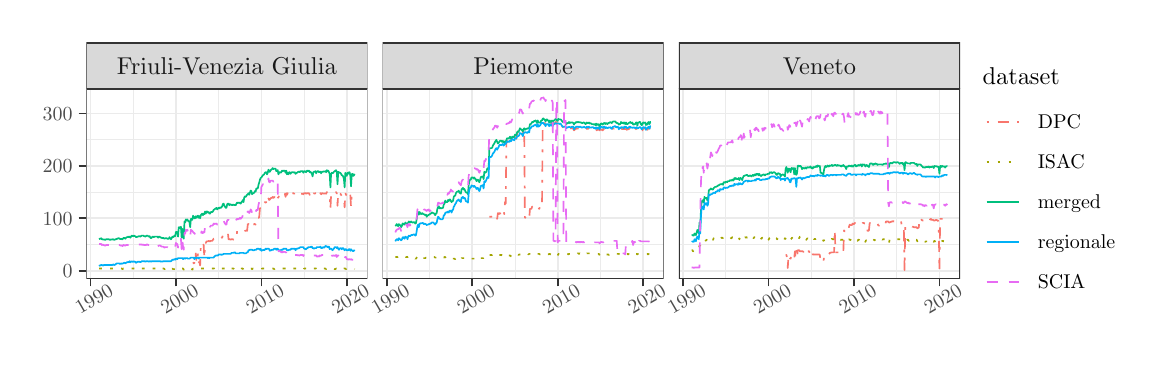
\begin{tikzpicture}[x=1pt,y=1pt]
\definecolor{fillColor}{RGB}{255,255,255}
\path[use as bounding box,fill=fillColor] (0,0) rectangle (398.34,113.81);
\begin{scope}
\path[clip] (  0.00,  0.00) rectangle (398.34,113.81);
\definecolor{drawColor}{RGB}{255,255,255}

\path[draw=drawColor,line width= 0.6pt,line join=round,line cap=round,fill=fillColor] (  0.00,  0.00) rectangle (398.34,113.81);
\end{scope}
\begin{scope}
\path[clip] ( 21.17, 23.07) rectangle (122.75, 91.74);
\definecolor{fillColor}{RGB}{255,255,255}

\path[fill=fillColor] ( 21.17, 23.07) rectangle (122.75, 91.74);
\definecolor{drawColor}{gray}{0.92}

\path[draw=drawColor,line width= 0.3pt,line join=round] ( 21.17, 35.46) --
	(122.75, 35.46);

\path[draw=drawColor,line width= 0.3pt,line join=round] ( 21.17, 54.38) --
	(122.75, 54.38);

\path[draw=drawColor,line width= 0.3pt,line join=round] ( 21.17, 73.29) --
	(122.75, 73.29);

\path[draw=drawColor,line width= 0.3pt,line join=round] ( 38.14, 23.07) --
	( 38.14, 91.74);

\path[draw=drawColor,line width= 0.3pt,line join=round] ( 69.01, 23.07) --
	( 69.01, 91.74);

\path[draw=drawColor,line width= 0.3pt,line join=round] ( 99.87, 23.07) --
	( 99.87, 91.74);

\path[draw=drawColor,line width= 0.6pt,line join=round] ( 21.17, 26.00) --
	(122.75, 26.00);

\path[draw=drawColor,line width= 0.6pt,line join=round] ( 21.17, 44.92) --
	(122.75, 44.92);

\path[draw=drawColor,line width= 0.6pt,line join=round] ( 21.17, 63.84) --
	(122.75, 63.84);

\path[draw=drawColor,line width= 0.6pt,line join=round] ( 21.17, 82.75) --
	(122.75, 82.75);

\path[draw=drawColor,line width= 0.6pt,line join=round] ( 22.71, 23.07) --
	( 22.71, 91.74);

\path[draw=drawColor,line width= 0.6pt,line join=round] ( 53.57, 23.07) --
	( 53.57, 91.74);

\path[draw=drawColor,line width= 0.6pt,line join=round] ( 84.44, 23.07) --
	( 84.44, 91.74);

\path[draw=drawColor,line width= 0.6pt,line join=round] (115.30, 23.07) --
	(115.30, 91.74);
\definecolor{drawColor}{RGB}{248,118,109}

\path[draw=drawColor,line width= 0.6pt,dash pattern=on 1pt off 3pt on 4pt off 3pt ,line join=round] ( 59.75, 29.03) --
	( 60.01, 28.65) --
	( 60.25, 28.84) --
	( 60.51, 28.27) --
	( 60.76, 32.24) --
	( 61.02, 29.03) --
	( 61.28, 29.03) --
	( 61.54, 32.24) --
	( 61.80, 29.03) --
	( 62.05, 29.03) --
	( 62.32, 27.89) --
	( 62.57, 35.84) --
	( 62.83, 35.46) --
	( 63.09, 35.84) --
	( 63.33, 35.65) --
	( 63.59, 35.27) --
	( 63.85, 30.54) --
	( 64.11, 36.22) --
	( 64.36, 36.03) --
	( 64.62, 36.60) --
	( 64.89, 36.60) --
	( 65.14, 36.60) --
	( 65.40, 36.78) --
	( 65.65, 36.60) --
	( 65.92, 36.60) --
	( 66.18, 36.78) --
	( 66.42, 36.78) --
	( 66.69, 36.78) --
	( 66.94, 37.16) --
	( 67.20, 37.54) --
	( 67.45, 37.54) --
	( 67.72, 37.54) --
	( 67.98, 37.54) --
	( 68.23, 37.54) --
	( 68.49, 37.35) --
	( 68.75, 37.54) --
	( 69.01, 37.54) --
	( 69.27, 37.54) --
	( 69.51, 37.54) --
	( 69.77, 37.54) --
	( 70.02, 37.92) --
	( 70.29, 37.92) --
	( 70.54, 38.87) --
	( 70.80, 39.05) --
	( 71.06, 39.24) --
	( 71.32, 39.05) --
	( 71.58, 39.24) --
	( 71.83, 39.62) --
	( 72.09, 39.81) --
	( 72.36, 39.62) --
	( 72.59, 37.35) --
	( 72.85, 37.35) --
	( 73.11, 37.35) --
	( 73.37, 37.16) --
	( 73.62, 37.35) --
	( 73.89, 37.35) --
	( 74.15, 37.35) --
	( 74.40, 37.16) --
	( 74.66, 37.16) --
	( 74.92, 37.16) --
	( 75.18, 37.16) --
	( 75.44, 37.35) --
	( 75.68, 40.38) --
	( 75.94, 40.38) --
	( 76.19, 40.38) --
	( 76.45, 40.38) --
	( 76.71, 40.38) --
	( 76.97, 40.38) --
	( 77.23, 40.19) --
	( 77.49, 40.19) --
	( 77.75, 40.00) --
	( 78.00, 40.19) --
	( 78.26, 40.19) --
	( 78.53, 40.38) --
	( 78.77, 40.38) --
	( 79.03, 40.57) --
	( 79.29, 40.38) --
	( 79.55, 42.84) --
	( 79.80, 42.84) --
	( 80.06, 42.65) --
	( 80.33, 42.84) --
	( 80.58, 42.84) --
	( 80.84, 42.84) --
	( 81.09, 41.89) --
	( 81.36, 42.65) --
	( 81.62, 42.65) --
	( 81.85, 42.84) --
	( 82.12, 42.84) --
	( 82.37, 42.65) --
	( 82.63, 45.11) --
	( 82.89, 45.11) --
	( 83.15, 45.11) --
	( 83.41, 45.11) --
	( 83.66, 45.30) --
	( 83.93, 48.51) --
	( 84.18, 48.70) --
	( 84.44, 48.70) --
	( 84.70, 48.70) --
	( 84.94, 48.70) --
	( 85.20, 48.70) --
	( 85.45, 50.40) --
	( 85.72, 50.78) --
	( 85.97, 50.59) --
	( 86.23, 50.78) --
	( 86.49, 49.84) --
	( 86.75, 50.03) --
	( 87.01, 52.11) --
	( 87.26, 51.54) --
	( 87.53, 51.73) --
	( 87.79, 52.11) --
	( 88.02, 52.30) --
	( 88.29, 52.30) --
	( 88.54, 52.67) --
	( 88.80, 52.30) --
	( 89.06, 52.67) --
	( 89.32, 52.49) --
	( 89.58, 52.49) --
	( 89.83, 51.92) --
	( 90.09, 50.97) --
	( 90.35, 52.30) --
	( 90.61, 52.49) --
	( 90.87, 53.24) --
	( 91.12, 53.24) --
	( 91.38, 52.86) --
	( 91.63, 53.24) --
	( 91.89, 53.81) --
	( 92.15, 54.00) --
	( 92.41, 53.81) --
	( 92.67, 53.81) --
	( 92.93, 53.81) --
	( 93.19, 52.67) --
	( 93.44, 54.00) --
	( 93.70, 53.43) --
	( 93.96, 54.00) --
	( 94.20, 53.43) --
	( 94.46, 54.00) --
	( 94.72, 54.00) --
	( 94.98, 53.43) --
	( 95.23, 53.62) --
	( 95.49, 54.00) --
	( 95.76, 54.00) --
	( 96.01, 54.00) --
	( 96.27, 53.81) --
	( 96.53, 54.00) --
	( 96.79, 53.62) --
	( 97.05, 53.24) --
	( 97.29, 53.43) --
	( 97.55, 53.62) --
	( 97.80, 53.62) --
	( 98.06, 53.81) --
	( 98.32, 53.62) --
	( 98.58, 53.81) --
	( 98.84, 53.81) --
	( 99.09, 53.81) --
	( 99.36, 53.81) --
	( 99.61, 53.62) --
	( 99.87, 54.00) --
	(100.13, 54.00) --
	(100.37, 54.00) --
	(100.63, 53.81) --
	(100.89, 54.00) --
	(101.15, 54.00) --
	(101.40, 54.00) --
	(101.66, 54.00) --
	(101.93, 53.43) --
	(102.18, 53.62) --
	(102.44, 53.43) --
	(102.69, 53.24) --
	(102.96, 52.49) --
	(103.22, 53.81) --
	(103.46, 54.00) --
	(103.73, 53.81) --
	(103.98, 54.00) --
	(104.24, 53.05) --
	(104.49, 54.00) --
	(104.76, 54.00) --
	(105.02, 54.00) --
	(105.27, 53.81) --
	(105.53, 53.81) --
	(105.79, 54.00) --
	(106.05, 53.62) --
	(106.31, 54.00) --
	(106.55, 54.00) --
	(106.81, 53.81) --
	(107.06, 54.00) --
	(107.33, 53.81) --
	(107.58, 54.00) --
	(107.84, 53.81) --
	(108.10, 54.38) --
	(108.36, 54.19) --
	(108.62, 54.19) --
	(108.87, 53.81) --
	(109.13, 53.81) --
	(109.40, 48.32) --
	(109.63, 53.24) --
	(109.89, 54.00) --
	(110.15, 54.19) --
	(110.41, 54.00) --
	(110.66, 54.38) --
	(110.93, 54.19) --
	(111.19, 54.38) --
	(111.44, 54.38) --
	(111.70, 54.00) --
	(111.96, 49.46) --
	(112.22, 54.19) --
	(112.48, 54.38) --
	(112.72, 53.81) --
	(112.98, 53.81) --
	(113.23, 53.43) --
	(113.49, 53.05) --
	(113.75, 52.86) --
	(114.01, 52.67) --
	(114.27, 52.11) --
	(114.53, 48.89) --
	(114.79, 54.19) --
	(115.04, 53.43) --
	(115.30, 53.24) --
	(115.57, 54.38) --
	(115.81, 54.00) --
	(116.07, 54.19) --
	(116.33, 54.19) --
	(116.59, 53.24) --
	(116.84, 49.08) --
	(117.10, 54.00) --
	(117.37, 54.38) --
	(117.62, 53.81) --
	(117.88, 53.81) --
	(118.13, 54.00);
\definecolor{drawColor}{RGB}{163,165,0}

\path[draw=drawColor,line width= 0.6pt,dash pattern=on 1pt off 3pt ,line join=round] ( 25.79, 26.76) --
	( 26.05, 26.76) --
	( 26.29, 26.76) --
	( 26.55, 26.76) --
	( 26.81, 26.76) --
	( 27.07, 26.76) --
	( 27.32, 26.76) --
	( 27.58, 26.76) --
	( 27.85, 26.76) --
	( 28.10, 26.76) --
	( 28.36, 26.76) --
	( 28.61, 26.76) --
	( 28.88, 26.76) --
	( 29.14, 26.76) --
	( 29.38, 26.76) --
	( 29.65, 26.76) --
	( 29.90, 26.76) --
	( 30.16, 26.76) --
	( 30.41, 26.76) --
	( 30.68, 26.76) --
	( 30.94, 26.76) --
	( 31.19, 26.76) --
	( 31.45, 26.76) --
	( 31.71, 26.76) --
	( 31.97, 26.76) --
	( 32.23, 26.76) --
	( 32.47, 26.76) --
	( 32.73, 26.76) --
	( 32.98, 26.76) --
	( 33.25, 26.76) --
	( 33.50, 26.76) --
	( 33.76, 26.76) --
	( 34.02, 26.76) --
	( 34.28, 26.57) --
	( 34.54, 26.76) --
	( 34.79, 26.76) --
	( 35.05, 26.76) --
	( 35.32, 26.76) --
	( 35.55, 26.76) --
	( 35.81, 26.76) --
	( 36.07, 26.76) --
	( 36.33, 26.76) --
	( 36.58, 26.76) --
	( 36.85, 26.57) --
	( 37.11, 26.76) --
	( 37.36, 26.76) --
	( 37.62, 26.76) --
	( 37.88, 26.76) --
	( 38.14, 26.76) --
	( 38.40, 26.76) --
	( 38.64, 26.76) --
	( 38.90, 26.76) --
	( 39.15, 26.76) --
	( 39.41, 26.57) --
	( 39.67, 26.76) --
	( 39.93, 26.57) --
	( 40.19, 26.76) --
	( 40.45, 26.76) --
	( 40.71, 26.76) --
	( 40.96, 26.76) --
	( 41.22, 26.76) --
	( 41.49, 26.76) --
	( 41.73, 26.76) --
	( 41.99, 26.76) --
	( 42.25, 26.76) --
	( 42.51, 26.76) --
	( 42.76, 26.76) --
	( 43.02, 26.76) --
	( 43.29, 26.76) --
	( 43.54, 26.76) --
	( 43.80, 26.76) --
	( 44.05, 26.76) --
	( 44.32, 26.76) --
	( 44.58, 26.76) --
	( 44.81, 26.57) --
	( 45.08, 26.76) --
	( 45.33, 26.76) --
	( 45.59, 26.76) --
	( 45.85, 26.76) --
	( 46.11, 26.76) --
	( 46.37, 26.76) --
	( 46.62, 26.57) --
	( 46.89, 26.76) --
	( 47.14, 26.57) --
	( 47.40, 26.76) --
	( 47.66, 26.76) --
	( 47.90, 26.57) --
	( 48.16, 26.57) --
	( 48.41, 26.76) --
	( 48.68, 26.76) --
	( 48.93, 26.76) --
	( 49.19, 26.76) --
	( 49.45, 26.57) --
	( 49.71, 26.76) --
	( 49.97, 26.76) --
	( 50.22, 26.76) --
	( 50.49, 26.57) --
	( 50.75, 26.76) --
	( 50.98, 26.76) --
	( 51.25, 26.76) --
	( 51.50, 26.76) --
	( 51.76, 26.38) --
	( 52.02, 26.57) --
	( 52.28, 26.76) --
	( 52.54, 26.57) --
	( 52.79, 26.57) --
	( 53.05, 26.57) --
	( 53.31, 26.57) --
	( 53.57, 26.76) --
	( 53.83, 26.76) --
	( 54.08, 26.76) --
	( 54.34, 26.38) --
	( 54.59, 26.57) --
	( 54.85, 26.76) --
	( 55.11, 26.76) --
	( 55.37, 26.76) --
	( 55.63, 26.76) --
	( 55.89, 26.76) --
	( 56.15, 26.76) --
	( 56.40, 26.38) --
	( 56.66, 26.76) --
	( 56.92, 26.76) --
	( 57.16, 26.76) --
	( 57.42, 26.57) --
	( 57.68, 26.76) --
	( 57.94, 26.76) --
	( 58.19, 26.76) --
	( 58.45, 26.76) --
	( 58.72, 26.76) --
	( 58.97, 26.76) --
	( 59.23, 26.76) --
	( 59.49, 26.38) --
	( 59.75, 26.76) --
	( 60.01, 26.76) --
	( 60.25, 26.76) --
	( 60.51, 26.76) --
	( 60.76, 26.76) --
	( 61.02, 26.57) --
	( 61.28, 26.76) --
	( 61.54, 26.76) --
	( 61.80, 26.76) --
	( 62.05, 26.76) --
	( 62.32, 26.76) --
	( 62.57, 26.76) --
	( 62.83, 26.76) --
	( 63.09, 26.76) --
	( 63.33, 26.76) --
	( 63.59, 26.76) --
	( 63.85, 26.76) --
	( 64.11, 26.76) --
	( 64.36, 26.76) --
	( 64.62, 26.76) --
	( 64.89, 26.76) --
	( 65.14, 26.76) --
	( 65.40, 26.76) --
	( 65.65, 26.57) --
	( 65.92, 26.57) --
	( 66.18, 26.76) --
	( 66.42, 26.76) --
	( 66.69, 26.76) --
	( 66.94, 26.76) --
	( 67.20, 26.76) --
	( 67.45, 26.76) --
	( 67.72, 26.57) --
	( 67.98, 26.76) --
	( 68.23, 26.76) --
	( 68.49, 26.57) --
	( 68.75, 26.76) --
	( 69.01, 26.76) --
	( 69.27, 26.57) --
	( 69.51, 26.76) --
	( 69.77, 26.76) --
	( 70.02, 26.76) --
	( 70.29, 26.76) --
	( 70.54, 26.76) --
	( 70.80, 26.76) --
	( 71.06, 26.76) --
	( 71.32, 26.76) --
	( 71.58, 26.76) --
	( 71.83, 26.57) --
	( 72.09, 26.57) --
	( 72.36, 26.76) --
	( 72.59, 26.76) --
	( 72.85, 26.38) --
	( 73.11, 26.76) --
	( 73.37, 26.76) --
	( 73.62, 26.76) --
	( 73.89, 26.76) --
	( 74.15, 26.76) --
	( 74.40, 26.76) --
	( 74.66, 26.57) --
	( 74.92, 26.38) --
	( 75.18, 26.76) --
	( 75.44, 26.76) --
	( 75.68, 26.76) --
	( 75.94, 26.57) --
	( 76.19, 26.76) --
	( 76.45, 26.76) --
	( 76.71, 26.76) --
	( 76.97, 26.57) --
	( 77.23, 26.76) --
	( 77.49, 26.76) --
	( 77.75, 26.76) --
	( 78.00, 26.38) --
	( 78.26, 26.57) --
	( 78.53, 26.76) --
	( 78.77, 26.76) --
	( 79.03, 26.76) --
	( 79.29, 26.76) --
	( 79.55, 26.76) --
	( 79.80, 26.76) --
	( 80.06, 26.57) --
	( 80.33, 26.76) --
	( 80.58, 26.76) --
	( 80.84, 26.76) --
	( 81.09, 26.57) --
	( 81.36, 26.76) --
	( 81.62, 26.76) --
	( 81.85, 26.76) --
	( 82.12, 26.76) --
	( 82.37, 26.76) --
	( 82.63, 26.76) --
	( 82.89, 26.76) --
	( 83.15, 26.76) --
	( 83.41, 26.76) --
	( 83.66, 26.76) --
	( 83.93, 26.76) --
	( 84.18, 26.76) --
	( 84.44, 26.57) --
	( 84.70, 26.76) --
	( 84.94, 26.76) --
	( 85.20, 26.76) --
	( 85.45, 26.76) --
	( 85.72, 26.76) --
	( 85.97, 26.76) --
	( 86.23, 26.76) --
	( 86.49, 26.76) --
	( 86.75, 26.76) --
	( 87.01, 26.76) --
	( 87.26, 26.76) --
	( 87.53, 26.76) --
	( 87.79, 26.76) --
	( 88.02, 26.76) --
	( 88.29, 26.76) --
	( 88.54, 26.76) --
	( 88.80, 26.76) --
	( 89.06, 26.57) --
	( 89.32, 26.76) --
	( 89.58, 26.76) --
	( 89.83, 26.76) --
	( 90.09, 26.76) --
	( 90.35, 26.57) --
	( 90.61, 26.76) --
	( 90.87, 26.76) --
	( 91.12, 26.76) --
	( 91.38, 26.76) --
	( 91.63, 26.76) --
	( 91.89, 26.76) --
	( 92.15, 26.76) --
	( 92.41, 26.76) --
	( 92.67, 26.76) --
	( 92.93, 26.76) --
	( 93.19, 26.76) --
	( 93.44, 26.57) --
	( 93.70, 26.76) --
	( 93.96, 26.76) --
	( 94.20, 26.76) --
	( 94.46, 26.76) --
	( 94.72, 26.76) --
	( 94.98, 26.76) --
	( 95.23, 26.76) --
	( 95.49, 26.76) --
	( 95.76, 26.76) --
	( 96.01, 26.76) --
	( 96.27, 26.76) --
	( 96.53, 26.76) --
	( 96.79, 26.76) --
	( 97.05, 26.76) --
	( 97.29, 26.76) --
	( 97.55, 26.76) --
	( 97.80, 26.76) --
	( 98.06, 26.76) --
	( 98.32, 26.76) --
	( 98.58, 26.76) --
	( 98.84, 26.76) --
	( 99.09, 26.76) --
	( 99.36, 26.76) --
	( 99.61, 26.38) --
	( 99.87, 26.76) --
	(100.13, 26.76) --
	(100.37, 26.76) --
	(100.63, 26.76) --
	(100.89, 26.76) --
	(101.15, 26.76) --
	(101.40, 26.57) --
	(101.66, 26.76) --
	(101.93, 26.76) --
	(102.18, 26.76) --
	(102.44, 26.76) --
	(102.69, 26.57) --
	(102.96, 26.57) --
	(103.22, 26.76) --
	(103.46, 26.76) --
	(103.73, 26.76) --
	(103.98, 26.76) --
	(104.24, 26.76) --
	(104.49, 26.57) --
	(104.76, 26.76) --
	(105.02, 26.76) --
	(105.27, 26.57) --
	(105.53, 26.76) --
	(105.79, 26.57) --
	(106.05, 26.57) --
	(106.31, 26.76) --
	(106.55, 26.76) --
	(106.81, 26.76) --
	(107.06, 26.76) --
	(107.33, 26.76) --
	(107.58, 26.76) --
	(107.84, 26.57) --
	(108.10, 26.76) --
	(108.36, 26.76) --
	(108.62, 26.76) --
	(108.87, 26.57) --
	(109.13, 26.57) --
	(109.40, 26.76) --
	(109.63, 26.76) --
	(109.89, 26.76) --
	(110.15, 26.76) --
	(110.41, 26.76) --
	(110.66, 26.76) --
	(110.93, 26.57) --
	(111.19, 26.57) --
	(111.44, 26.76) --
	(111.70, 26.76) --
	(111.96, 26.57) --
	(112.22, 26.76) --
	(112.48, 26.76) --
	(112.72, 26.76) --
	(112.98, 26.57) --
	(113.23, 26.57) --
	(113.49, 26.76) --
	(113.75, 26.76) --
	(114.01, 26.57) --
	(114.27, 26.76) --
	(114.53, 26.76) --
	(114.79, 26.76) --
	(115.04, 26.57) --
	(115.30, 26.76) --
	(115.57, 26.76) --
	(115.81, 26.76) --
	(116.07, 26.76) --
	(116.33, 26.76) --
	(116.59, 26.76) --
	(116.84, 26.76) --
	(117.10, 26.76) --
	(117.37, 26.76) --
	(117.62, 26.76) --
	(117.88, 26.76) --
	(118.13, 26.57);
\definecolor{drawColor}{RGB}{0,191,125}

\path[draw=drawColor,line width= 0.6pt,line join=round] ( 25.79, 37.35) --
	( 26.05, 37.54) --
	( 26.29, 37.54) --
	( 26.55, 37.73) --
	( 26.81, 37.35) --
	( 27.07, 37.35) --
	( 27.32, 37.16) --
	( 27.58, 37.35) --
	( 27.85, 37.16) --
	( 28.10, 37.16) --
	( 28.36, 37.35) --
	( 28.61, 37.35) --
	( 28.88, 37.35) --
	( 29.14, 37.35) --
	( 29.38, 37.35) --
	( 29.65, 37.16) --
	( 29.90, 37.16) --
	( 30.16, 37.35) --
	( 30.41, 37.16) --
	( 30.68, 37.35) --
	( 30.94, 37.35) --
	( 31.19, 37.16) --
	( 31.45, 37.16) --
	( 31.71, 37.35) --
	( 31.97, 37.35) --
	( 32.23, 37.54) --
	( 32.47, 37.54) --
	( 32.73, 37.73) --
	( 32.98, 37.73) --
	( 33.25, 37.54) --
	( 33.50, 37.35) --
	( 33.76, 37.54) --
	( 34.02, 37.35) --
	( 34.28, 37.35) --
	( 34.54, 37.73) --
	( 34.79, 37.92) --
	( 35.05, 37.73) --
	( 35.32, 37.54) --
	( 35.55, 37.92) --
	( 35.81, 38.11) --
	( 36.07, 38.11) --
	( 36.33, 38.30) --
	( 36.58, 38.11) --
	( 36.85, 38.30) --
	( 37.11, 37.92) --
	( 37.36, 38.30) --
	( 37.62, 38.68) --
	( 37.88, 38.49) --
	( 38.14, 38.49) --
	( 38.40, 38.68) --
	( 38.64, 38.49) --
	( 38.90, 38.49) --
	( 39.15, 38.11) --
	( 39.41, 38.11) --
	( 39.67, 38.30) --
	( 39.93, 38.30) --
	( 40.19, 38.49) --
	( 40.45, 38.49) --
	( 40.71, 38.30) --
	( 40.96, 38.49) --
	( 41.22, 38.68) --
	( 41.49, 38.68) --
	( 41.73, 38.68) --
	( 41.99, 38.49) --
	( 42.25, 38.49) --
	( 42.51, 38.30) --
	( 42.76, 38.49) --
	( 43.02, 38.68) --
	( 43.29, 38.68) --
	( 43.54, 38.49) --
	( 43.80, 38.30) --
	( 44.05, 38.49) --
	( 44.32, 37.92) --
	( 44.58, 37.73) --
	( 44.81, 37.92) --
	( 45.08, 38.30) --
	( 45.33, 38.30) --
	( 45.59, 38.11) --
	( 45.85, 38.30) --
	( 46.11, 38.30) --
	( 46.37, 38.30) --
	( 46.62, 38.30) --
	( 46.89, 38.30) --
	( 47.14, 37.92) --
	( 47.40, 38.30) --
	( 47.66, 38.30) --
	( 47.90, 38.11) --
	( 48.16, 37.92) --
	( 48.41, 37.92) --
	( 48.68, 37.73) --
	( 48.93, 37.92) --
	( 49.19, 37.73) --
	( 49.45, 37.54) --
	( 49.71, 37.73) --
	( 49.97, 37.73) --
	( 50.22, 37.73) --
	( 50.49, 37.54) --
	( 50.75, 37.54) --
	( 50.98, 37.54) --
	( 51.25, 38.11) --
	( 51.50, 37.73) --
	( 51.76, 37.35) --
	( 52.02, 37.73) --
	( 52.28, 38.30) --
	( 52.54, 38.11) --
	( 52.79, 38.30) --
	( 53.05, 38.68) --
	( 53.31, 38.49) --
	( 53.57, 40.00) --
	( 53.83, 40.00) --
	( 54.08, 39.81) --
	( 54.34, 38.30) --
	( 54.59, 41.70) --
	( 54.85, 41.70) --
	( 55.11, 41.32) --
	( 55.37, 41.89) --
	( 55.63, 37.92) --
	( 55.89, 41.14) --
	( 56.15, 38.30) --
	( 56.40, 37.54) --
	( 56.66, 43.78) --
	( 56.92, 43.41) --
	( 57.16, 44.54) --
	( 57.42, 44.16) --
	( 57.68, 44.54) --
	( 57.94, 43.97) --
	( 58.19, 43.97) --
	( 58.45, 43.59) --
	( 58.72, 41.70) --
	( 58.97, 44.73) --
	( 59.23, 44.73) --
	( 59.49, 44.35) --
	( 59.75, 45.86) --
	( 60.01, 45.49) --
	( 60.25, 44.92) --
	( 60.51, 44.92) --
	( 60.76, 45.68) --
	( 61.02, 45.11) --
	( 61.28, 45.68) --
	( 61.54, 45.86) --
	( 61.80, 45.11) --
	( 62.05, 45.68) --
	( 62.32, 44.92) --
	( 62.57, 46.05) --
	( 62.83, 46.43) --
	( 63.09, 46.62) --
	( 63.33, 46.05) --
	( 63.59, 46.62) --
	( 63.85, 46.43) --
	( 64.11, 47.38) --
	( 64.36, 46.62) --
	( 64.62, 47.38) --
	( 64.89, 47.38) --
	( 65.14, 47.00) --
	( 65.40, 47.19) --
	( 65.65, 46.62) --
	( 65.92, 46.62) --
	( 66.18, 47.19) --
	( 66.42, 47.19) --
	( 66.69, 47.19) --
	( 66.94, 47.38) --
	( 67.20, 47.95) --
	( 67.45, 48.13) --
	( 67.72, 48.32) --
	( 67.98, 48.51) --
	( 68.23, 48.70) --
	( 68.49, 48.13) --
	( 68.75, 48.51) --
	( 69.01, 48.70) --
	( 69.27, 48.51) --
	( 69.51, 48.89) --
	( 69.77, 48.70) --
	( 70.02, 48.89) --
	( 70.29, 49.27) --
	( 70.54, 50.03) --
	( 70.80, 50.22) --
	( 71.06, 49.46) --
	( 71.32, 49.08) --
	( 71.58, 48.70) --
	( 71.83, 48.70) --
	( 72.09, 50.03) --
	( 72.36, 50.22) --
	( 72.59, 50.22) --
	( 72.85, 49.65) --
	( 73.11, 50.03) --
	( 73.37, 49.84) --
	( 73.62, 49.84) --
	( 73.89, 49.65) --
	( 74.15, 49.84) --
	( 74.40, 49.84) --
	( 74.66, 49.65) --
	( 74.92, 49.84) --
	( 75.18, 49.65) --
	( 75.44, 50.22) --
	( 75.68, 50.59) --
	( 75.94, 50.40) --
	( 76.19, 50.59) --
	( 76.45, 50.59) --
	( 76.71, 50.40) --
	( 76.97, 50.22) --
	( 77.23, 50.78) --
	( 77.49, 50.97) --
	( 77.75, 51.54) --
	( 78.00, 50.78) --
	( 78.26, 52.49) --
	( 78.53, 52.86) --
	( 78.77, 52.67) --
	( 79.03, 53.05) --
	( 79.29, 53.43) --
	( 79.55, 53.62) --
	( 79.80, 54.00) --
	( 80.06, 53.43) --
	( 80.33, 54.19) --
	( 80.58, 54.94) --
	( 80.84, 54.76) --
	( 81.09, 53.62) --
	( 81.36, 54.00) --
	( 81.62, 54.00) --
	( 81.85, 54.19) --
	( 82.12, 54.76) --
	( 82.37, 54.57) --
	( 82.63, 55.70) --
	( 82.89, 55.70) --
	( 83.15, 55.70) --
	( 83.41, 57.03) --
	( 83.66, 57.78) --
	( 83.93, 58.92) --
	( 84.18, 59.48) --
	( 84.44, 59.67) --
	( 84.70, 60.05) --
	( 84.94, 60.43) --
	( 85.20, 60.62) --
	( 85.45, 60.81) --
	( 85.72, 61.38) --
	( 85.97, 61.57) --
	( 86.23, 61.57) --
	( 86.49, 60.81) --
	( 86.75, 61.38) --
	( 87.01, 62.51) --
	( 87.26, 61.75) --
	( 87.53, 61.75) --
	( 87.79, 62.32) --
	( 88.02, 62.51) --
	( 88.29, 62.70) --
	( 88.54, 63.08) --
	( 88.80, 62.70) --
	( 89.06, 62.89) --
	( 89.32, 62.89) --
	( 89.58, 62.89) --
	( 89.83, 61.94) --
	( 90.09, 62.13) --
	( 90.35, 62.32) --
	( 90.61, 60.81) --
	( 90.87, 61.57) --
	( 91.12, 61.57) --
	( 91.38, 61.38) --
	( 91.63, 61.57) --
	( 91.89, 62.13) --
	( 92.15, 61.94) --
	( 92.41, 62.13) --
	( 92.67, 62.13) --
	( 92.93, 62.13) --
	( 93.19, 61.38) --
	( 93.44, 62.13) --
	( 93.70, 60.81) --
	( 93.96, 61.38) --
	( 94.20, 60.81) --
	( 94.46, 61.57) --
	( 94.72, 61.57) --
	( 94.98, 61.00) --
	( 95.23, 61.38) --
	( 95.49, 61.57) --
	( 95.76, 61.57) --
	( 96.01, 61.57) --
	( 96.27, 61.38) --
	( 96.53, 61.57) --
	( 96.79, 61.00) --
	( 97.05, 61.19) --
	( 97.29, 61.38) --
	( 97.55, 61.57) --
	( 97.80, 61.75) --
	( 98.06, 61.75) --
	( 98.32, 61.57) --
	( 98.58, 61.94) --
	( 98.84, 61.94) --
	( 99.09, 61.94) --
	( 99.36, 61.94) --
	( 99.61, 61.38) --
	( 99.87, 61.94) --
	(100.13, 61.94) --
	(100.37, 61.75) --
	(100.63, 61.57) --
	(100.89, 62.13) --
	(101.15, 62.13) --
	(101.40, 61.94) --
	(101.66, 62.13) --
	(101.93, 61.57) --
	(102.18, 61.75) --
	(102.44, 61.38) --
	(102.69, 61.00) --
	(102.96, 60.05) --
	(103.22, 61.57) --
	(103.46, 61.75) --
	(103.73, 61.75) --
	(103.98, 61.94) --
	(104.24, 61.19) --
	(104.49, 61.75) --
	(104.76, 61.94) --
	(105.02, 61.94) --
	(105.27, 61.57) --
	(105.53, 61.75) --
	(105.79, 61.75) --
	(106.05, 61.19) --
	(106.31, 61.75) --
	(106.55, 61.75) --
	(106.81, 61.75) --
	(107.06, 61.94) --
	(107.33, 61.75) --
	(107.58, 61.94) --
	(107.84, 61.57) --
	(108.10, 62.32) --
	(108.36, 61.94) --
	(108.62, 62.13) --
	(108.87, 61.57) --
	(109.13, 61.00) --
	(109.40, 56.08) --
	(109.63, 60.81) --
	(109.89, 61.38) --
	(110.15, 61.19) --
	(110.41, 61.38) --
	(110.66, 61.75) --
	(110.93, 61.94) --
	(111.19, 62.13) --
	(111.44, 62.32) --
	(111.70, 61.57) --
	(111.96, 57.21) --
	(112.22, 61.75) --
	(112.48, 61.57) --
	(112.72, 61.38) --
	(112.98, 61.38) --
	(113.23, 61.00) --
	(113.49, 60.43) --
	(113.75, 60.43) --
	(114.01, 60.05) --
	(114.27, 59.11) --
	(114.53, 56.08) --
	(114.79, 61.38) --
	(115.04, 60.43) --
	(115.30, 60.24) --
	(115.57, 61.38) --
	(115.81, 61.00) --
	(116.07, 61.57) --
	(116.33, 61.57) --
	(116.59, 60.24) --
	(116.84, 56.46) --
	(117.10, 60.81) --
	(117.37, 61.00) --
	(117.62, 60.24) --
	(117.88, 60.43) --
	(118.13, 61.00);
\definecolor{drawColor}{RGB}{0,176,246}

\path[draw=drawColor,line width= 0.6pt,line join=round] ( 25.79, 27.70) --
	( 26.05, 27.89) --
	( 26.29, 27.89) --
	( 26.55, 28.08) --
	( 26.81, 28.08) --
	( 27.07, 27.89) --
	( 27.32, 27.89) --
	( 27.58, 28.08) --
	( 27.85, 28.08) --
	( 28.10, 28.08) --
	( 28.36, 28.08) --
	( 28.61, 28.08) --
	( 28.88, 28.08) --
	( 29.14, 28.08) --
	( 29.38, 28.08) --
	( 29.65, 28.08) --
	( 29.90, 28.08) --
	( 30.16, 28.08) --
	( 30.41, 28.08) --
	( 30.68, 28.08) --
	( 30.94, 28.27) --
	( 31.19, 28.08) --
	( 31.45, 28.08) --
	( 31.71, 28.27) --
	( 31.97, 28.46) --
	( 32.23, 28.65) --
	( 32.47, 28.65) --
	( 32.73, 28.65) --
	( 32.98, 28.65) --
	( 33.25, 28.46) --
	( 33.50, 28.46) --
	( 33.76, 28.65) --
	( 34.02, 28.46) --
	( 34.28, 28.65) --
	( 34.54, 28.65) --
	( 34.79, 28.84) --
	( 35.05, 28.84) --
	( 35.32, 28.65) --
	( 35.55, 28.84) --
	( 35.81, 29.03) --
	( 36.07, 29.03) --
	( 36.33, 29.22) --
	( 36.58, 29.03) --
	( 36.85, 29.41) --
	( 37.11, 29.03) --
	( 37.36, 29.22) --
	( 37.62, 29.41) --
	( 37.88, 29.22) --
	( 38.14, 29.22) --
	( 38.40, 29.41) --
	( 38.64, 29.22) --
	( 38.90, 29.22) --
	( 39.15, 28.84) --
	( 39.41, 29.03) --
	( 39.67, 29.22) --
	( 39.93, 29.22) --
	( 40.19, 29.22) --
	( 40.45, 29.22) --
	( 40.71, 29.03) --
	( 40.96, 29.22) --
	( 41.22, 29.41) --
	( 41.49, 29.41) --
	( 41.73, 29.41) --
	( 41.99, 29.41) --
	( 42.25, 29.41) --
	( 42.51, 29.22) --
	( 42.76, 29.41) --
	( 43.02, 29.41) --
	( 43.29, 29.41) --
	( 43.54, 29.41) --
	( 43.80, 29.22) --
	( 44.05, 29.41) --
	( 44.32, 29.41) --
	( 44.58, 29.22) --
	( 44.81, 29.41) --
	( 45.08, 29.41) --
	( 45.33, 29.41) --
	( 45.59, 29.41) --
	( 45.85, 29.41) --
	( 46.11, 29.41) --
	( 46.37, 29.41) --
	( 46.62, 29.41) --
	( 46.89, 29.41) --
	( 47.14, 29.41) --
	( 47.40, 29.41) --
	( 47.66, 29.41) --
	( 47.90, 29.41) --
	( 48.16, 29.22) --
	( 48.41, 29.41) --
	( 48.68, 29.22) --
	( 48.93, 29.41) --
	( 49.19, 29.41) --
	( 49.45, 29.41) --
	( 49.71, 29.41) --
	( 49.97, 29.41) --
	( 50.22, 29.41) --
	( 50.49, 29.41) --
	( 50.75, 29.41) --
	( 50.98, 29.41) --
	( 51.25, 29.41) --
	( 51.50, 29.41) --
	( 51.76, 29.41) --
	( 52.02, 29.60) --
	( 52.28, 29.97) --
	( 52.54, 29.97) --
	( 52.79, 29.97) --
	( 53.05, 30.16) --
	( 53.31, 29.97) --
	( 53.57, 30.35) --
	( 53.83, 30.35) --
	( 54.08, 30.16) --
	( 54.34, 30.54) --
	( 54.59, 30.54) --
	( 54.85, 30.54) --
	( 55.11, 30.54) --
	( 55.37, 30.54) --
	( 55.63, 30.54) --
	( 55.89, 30.54) --
	( 56.15, 30.16) --
	( 56.40, 30.54) --
	( 56.66, 30.54) --
	( 56.92, 30.35) --
	( 57.16, 30.54) --
	( 57.42, 30.54) --
	( 57.68, 30.54) --
	( 57.94, 30.35) --
	( 58.19, 30.35) --
	( 58.45, 30.35) --
	( 58.72, 30.54) --
	( 58.97, 30.73) --
	( 59.23, 30.73) --
	( 59.49, 30.73) --
	( 59.75, 30.73) --
	( 60.01, 30.73) --
	( 60.25, 30.16) --
	( 60.51, 30.73) --
	( 60.76, 30.73) --
	( 61.02, 30.54) --
	( 61.28, 30.73) --
	( 61.54, 30.73) --
	( 61.80, 30.35) --
	( 62.05, 30.73) --
	( 62.32, 30.73) --
	( 62.57, 30.73) --
	( 62.83, 30.73) --
	( 63.09, 30.73) --
	( 63.33, 30.73) --
	( 63.59, 30.73) --
	( 63.85, 30.73) --
	( 64.11, 30.73) --
	( 64.36, 30.73) --
	( 64.62, 30.73) --
	( 64.89, 30.73) --
	( 65.14, 30.54) --
	( 65.40, 30.73) --
	( 65.65, 30.54) --
	( 65.92, 30.73) --
	( 66.18, 30.73) --
	( 66.42, 30.73) --
	( 66.69, 30.73) --
	( 66.94, 30.73) --
	( 67.20, 30.73) --
	( 67.45, 31.11) --
	( 67.72, 31.30) --
	( 67.98, 31.49) --
	( 68.23, 31.49) --
	( 68.49, 31.49) --
	( 68.75, 31.49) --
	( 69.01, 31.87) --
	( 69.27, 31.87) --
	( 69.51, 31.87) --
	( 69.77, 31.87) --
	( 70.02, 31.68) --
	( 70.29, 31.87) --
	( 70.54, 31.87) --
	( 70.80, 32.06) --
	( 71.06, 32.06) --
	( 71.32, 32.06) --
	( 71.58, 32.06) --
	( 71.83, 32.06) --
	( 72.09, 32.06) --
	( 72.36, 32.06) --
	( 72.59, 32.06) --
	( 72.85, 32.06) --
	( 73.11, 32.06) --
	( 73.37, 32.06) --
	( 73.62, 32.43) --
	( 73.89, 32.43) --
	( 74.15, 32.43) --
	( 74.40, 32.43) --
	( 74.66, 32.62) --
	( 74.92, 32.62) --
	( 75.18, 32.24) --
	( 75.44, 32.24) --
	( 75.68, 32.24) --
	( 75.94, 32.24) --
	( 76.19, 32.24) --
	( 76.45, 32.24) --
	( 76.71, 32.43) --
	( 76.97, 32.43) --
	( 77.23, 32.43) --
	( 77.49, 32.43) --
	( 77.75, 32.43) --
	( 78.00, 32.43) --
	( 78.26, 32.24) --
	( 78.53, 32.24) --
	( 78.77, 32.24) --
	( 79.03, 32.43) --
	( 79.29, 32.62) --
	( 79.55, 32.62) --
	( 79.80, 33.38) --
	( 80.06, 33.38) --
	( 80.33, 33.57) --
	( 80.58, 33.57) --
	( 80.84, 33.57) --
	( 81.09, 33.57) --
	( 81.36, 33.38) --
	( 81.62, 33.38) --
	( 81.85, 33.38) --
	( 82.12, 33.57) --
	( 82.37, 33.57) --
	( 82.63, 33.57) --
	( 82.89, 33.95) --
	( 83.15, 33.95) --
	( 83.41, 33.95) --
	( 83.66, 33.76) --
	( 83.93, 33.57) --
	( 84.18, 33.95) --
	( 84.44, 33.19) --
	( 84.70, 33.38) --
	( 84.94, 33.38) --
	( 85.20, 33.57) --
	( 85.45, 33.38) --
	( 85.72, 33.57) --
	( 85.97, 33.95) --
	( 86.23, 33.76) --
	( 86.49, 33.95) --
	( 86.75, 33.95) --
	( 87.01, 33.95) --
	( 87.26, 33.76) --
	( 87.53, 33.19) --
	( 87.79, 33.38) --
	( 88.02, 33.38) --
	( 88.29, 33.57) --
	( 88.54, 33.57) --
	( 88.80, 33.57) --
	( 89.06, 33.95) --
	( 89.32, 33.95) --
	( 89.58, 33.95) --
	( 89.83, 33.57) --
	( 90.09, 33.95) --
	( 90.35, 33.95) --
	( 90.61, 33.38) --
	( 90.87, 33.38) --
	( 91.12, 33.38) --
	( 91.38, 33.38) --
	( 91.63, 33.57) --
	( 91.89, 33.57) --
	( 92.15, 33.57) --
	( 92.41, 33.95) --
	( 92.67, 33.95) --
	( 92.93, 33.95) --
	( 93.19, 33.95) --
	( 93.44, 33.95) --
	( 93.70, 33.38) --
	( 93.96, 33.38) --
	( 94.20, 33.38) --
	( 94.46, 33.57) --
	( 94.72, 33.57) --
	( 94.98, 33.57) --
	( 95.23, 33.95) --
	( 95.49, 33.95) --
	( 95.76, 33.95) --
	( 96.01, 33.95) --
	( 96.27, 33.95) --
	( 96.53, 33.95) --
	( 96.79, 33.38) --
	( 97.05, 33.95) --
	( 97.29, 33.95) --
	( 97.55, 33.95) --
	( 97.80, 34.14) --
	( 98.06, 34.14) --
	( 98.32, 34.33) --
	( 98.58, 34.51) --
	( 98.84, 34.51) --
	( 99.09, 34.51) --
	( 99.36, 34.51) --
	( 99.61, 34.51) --
	( 99.87, 33.95) --
	(100.13, 33.95) --
	(100.37, 33.76) --
	(100.63, 33.76) --
	(100.89, 34.14) --
	(101.15, 34.14) --
	(101.40, 34.51) --
	(101.66, 34.51) --
	(101.93, 34.51) --
	(102.18, 34.51) --
	(102.44, 34.70) --
	(102.69, 34.70) --
	(102.96, 34.14) --
	(103.22, 34.14) --
	(103.46, 33.95) --
	(103.73, 34.14) --
	(103.98, 34.14) --
	(104.24, 34.14) --
	(104.49, 34.51) --
	(104.76, 34.51) --
	(105.02, 34.51) --
	(105.27, 34.51) --
	(105.53, 34.51) --
	(105.79, 34.70) --
	(106.05, 34.14) --
	(106.31, 34.14) --
	(106.55, 34.33) --
	(106.81, 34.51) --
	(107.06, 34.33) --
	(107.33, 34.51) --
	(107.58, 34.89) --
	(107.84, 34.89) --
	(108.10, 34.70) --
	(108.36, 34.51) --
	(108.62, 34.70) --
	(108.87, 34.70) --
	(109.13, 33.76) --
	(109.40, 33.95) --
	(109.63, 33.95) --
	(109.89, 33.76) --
	(110.15, 33.38) --
	(110.41, 33.76) --
	(110.66, 33.95) --
	(110.93, 34.51) --
	(111.19, 34.51) --
	(111.44, 34.51) --
	(111.70, 34.14) --
	(111.96, 34.51) --
	(112.22, 33.95) --
	(112.48, 33.57) --
	(112.72, 33.95) --
	(112.98, 34.14) --
	(113.23, 34.14) --
	(113.49, 33.76) --
	(113.75, 34.14) --
	(114.01, 34.14) --
	(114.27, 33.76) --
	(114.53, 33.38) --
	(114.79, 33.76) --
	(115.04, 33.76) --
	(115.30, 33.38) --
	(115.57, 33.38) --
	(115.81, 33.38) --
	(116.07, 33.76) --
	(116.33, 33.76) --
	(116.59, 33.19) --
	(116.84, 33.76) --
	(117.10, 33.38) --
	(117.37, 33.19) --
	(117.62, 33.00) --
	(117.88, 33.19) --
	(118.13, 33.57);
\definecolor{drawColor}{RGB}{231,107,243}

\path[draw=drawColor,line width= 0.6pt,dash pattern=on 4pt off 4pt ,line join=round] ( 25.79, 35.65) --
	( 26.05, 35.65) --
	( 26.29, 35.65) --
	( 26.55, 35.65) --
	( 26.81, 35.27) --
	( 27.07, 35.46) --
	( 27.32, 35.27) --
	( 27.58, 35.27) --
	( 27.85, 35.08) --
	( 28.10, 35.08) --
	( 28.36, 35.27) --
	( 28.61, 35.27) --
	( 28.88, 35.27) --
	( 29.14, 35.27) --
	( 29.38, 35.27) --
	( 29.65, 35.08) --
	( 29.90, 35.08) --
	( 30.16, 35.27) --
	( 30.41, 35.08) --
	( 30.68, 35.27) --
	( 30.94, 35.08) --
	( 31.19, 35.08) --
	( 31.45, 35.08) --
	( 31.71, 35.08) --
	( 31.97, 35.08) --
	( 32.23, 35.08) --
	( 32.47, 35.08) --
	( 32.73, 35.27) --
	( 32.98, 35.27) --
	( 33.25, 35.27) --
	( 33.50, 35.08) --
	( 33.76, 35.08) --
	( 34.02, 35.08) --
	( 34.28, 34.89) --
	( 34.54, 35.27) --
	( 34.79, 35.27) --
	( 35.05, 35.08) --
	( 35.32, 35.08) --
	( 35.55, 35.27) --
	( 35.81, 35.27) --
	( 36.07, 35.27) --
	( 36.33, 35.27) --
	( 36.58, 35.27) --
	( 36.85, 35.08) --
	( 37.11, 35.08) --
	( 37.36, 35.27) --
	( 37.62, 35.46) --
	( 37.88, 35.46) --
	( 38.14, 35.46) --
	( 38.40, 35.46) --
	( 38.64, 35.46) --
	( 38.90, 35.46) --
	( 39.15, 35.46) --
	( 39.41, 35.27) --
	( 39.67, 35.27) --
	( 39.93, 35.27) --
	( 40.19, 35.46) --
	( 40.45, 35.46) --
	( 40.71, 35.46) --
	( 40.96, 35.46) --
	( 41.22, 35.46) --
	( 41.49, 35.27) --
	( 41.73, 35.46) --
	( 41.99, 35.27) --
	( 42.25, 35.27) --
	( 42.51, 35.27) --
	( 42.76, 35.27) --
	( 43.02, 35.46) --
	( 43.29, 35.46) --
	( 43.54, 35.27) --
	( 43.80, 35.27) --
	( 44.05, 35.27) --
	( 44.32, 34.70) --
	( 44.58, 34.70) --
	( 44.81, 34.70) --
	( 45.08, 35.08) --
	( 45.33, 35.08) --
	( 45.59, 34.89) --
	( 45.85, 35.08) --
	( 46.11, 35.08) --
	( 46.37, 35.08) --
	( 46.62, 34.89) --
	( 46.89, 34.70) --
	( 47.14, 34.89) --
	( 47.40, 35.08) --
	( 47.66, 35.08) --
	( 47.90, 35.08) --
	( 48.16, 34.89) --
	( 48.41, 34.70) --
	( 48.68, 34.70) --
	( 48.93, 34.70) --
	( 49.19, 34.51) --
	( 49.45, 34.33) --
	( 49.71, 34.51) --
	( 49.97, 34.51) --
	( 50.22, 34.51) --
	( 50.49, 34.51) --
	( 50.75, 34.33) --
	( 50.98, 34.33) --
	( 51.25, 34.89) --
	( 51.50, 34.33) --
	( 51.76, 33.95) --
	( 52.02, 34.14) --
	( 52.28, 34.33) --
	( 52.54, 34.14) --
	( 52.79, 34.33) --
	( 53.05, 34.51) --
	( 53.31, 34.70) --
	( 53.57, 36.03) --
	( 53.83, 35.65) --
	( 54.08, 35.65) --
	( 54.34, 34.33) --
	( 54.59, 37.54) --
	( 54.85, 37.35) --
	( 55.11, 36.97) --
	( 55.37, 37.54) --
	( 55.63, 33.76) --
	( 55.89, 37.16) --
	( 56.15, 34.51) --
	( 56.40, 33.57) --
	( 56.66, 39.62) --
	( 56.92, 39.43) --
	( 57.16, 40.76) --
	( 57.42, 40.38) --
	( 57.68, 40.76) --
	( 57.94, 40.38) --
	( 58.19, 40.38) --
	( 58.45, 40.00) --
	( 58.72, 37.92) --
	( 58.97, 40.76) --
	( 59.23, 40.57) --
	( 59.49, 40.38) --
	( 59.75, 40.00) --
	( 60.01, 39.62) --
	( 60.25, 39.62) --
	( 60.51, 39.05) --
	( 60.76, 39.62) --
	( 61.02, 39.62) --
	( 61.28, 39.43) --
	( 61.54, 39.81) --
	( 61.80, 39.24) --
	( 62.05, 39.62) --
	( 62.32, 39.43) --
	( 62.57, 39.05) --
	( 62.83, 40.19) --
	( 63.09, 39.62) --
	( 63.33, 39.62) --
	( 63.59, 40.00) --
	( 63.85, 39.81) --
	( 64.11, 42.08) --
	( 64.36, 41.14) --
	( 64.62, 42.08) --
	( 64.89, 41.89) --
	( 65.14, 42.08) --
	( 65.40, 42.27) --
	( 65.65, 42.08) --
	( 65.92, 41.89) --
	( 66.18, 42.27) --
	( 66.42, 42.27) --
	( 66.69, 42.27) --
	( 66.94, 42.46) --
	( 67.20, 43.03) --
	( 67.45, 42.84) --
	( 67.72, 43.03) --
	( 67.98, 42.84) --
	( 68.23, 43.03) --
	( 68.49, 42.65) --
	( 68.75, 42.84) --
	( 69.01, 42.84) --
	( 69.27, 42.84) --
	( 69.51, 43.03) --
	( 69.77, 42.65) --
	( 70.02, 43.22) --
	( 70.29, 43.41) --
	( 70.54, 43.97) --
	( 70.80, 44.35) --
	( 71.06, 43.41) --
	( 71.32, 43.03) --
	( 71.58, 42.65) --
	( 71.83, 42.65) --
	( 72.09, 44.16) --
	( 72.36, 44.35) --
	( 72.59, 44.35) --
	( 72.85, 44.16) --
	( 73.11, 44.35) --
	( 73.37, 43.97) --
	( 73.62, 43.97) --
	( 73.89, 43.59) --
	( 74.15, 44.16) --
	( 74.40, 44.35) --
	( 74.66, 44.35) --
	( 74.92, 44.54) --
	( 75.18, 43.97) --
	( 75.44, 44.54) --
	( 75.68, 44.73) --
	( 75.94, 44.54) --
	( 76.19, 44.73) --
	( 76.45, 44.73) --
	( 76.71, 45.11) --
	( 76.97, 44.73) --
	( 77.23, 45.11) --
	( 77.49, 45.30) --
	( 77.75, 46.05) --
	( 78.00, 45.11) --
	( 78.26, 46.62) --
	( 78.53, 47.19) --
	( 78.77, 47.00) --
	( 79.03, 47.19) --
	( 79.29, 47.19) --
	( 79.55, 47.38) --
	( 79.80, 47.38) --
	( 80.06, 46.81) --
	( 80.33, 47.38) --
	( 80.58, 48.13) --
	( 80.84, 47.76) --
	( 81.09, 46.81) --
	( 81.36, 47.38) --
	( 81.62, 46.24) --
	( 81.85, 47.00) --
	( 82.12, 47.57) --
	( 82.37, 47.19) --
	( 82.63, 47.95) --
	( 82.89, 47.95) --
	( 83.15, 47.95) --
	( 83.41, 49.84) --
	( 83.66, 50.78) --
	( 83.93, 50.78) --
	( 84.18, 50.40) --
	( 84.44, 56.27) --
	( 84.70, 56.65) --
	( 84.94, 57.21) --
	( 85.20, 57.21) --
	( 85.45, 57.21) --
	( 85.72, 57.40) --
	( 85.97, 57.59) --
	( 86.23, 57.59) --
	( 86.49, 56.84) --
	( 86.75, 58.35) --
	( 87.01, 59.30) --
	( 87.26, 57.97) --
	( 87.53, 57.97) --
	( 87.79, 58.54) --
	( 88.02, 58.54) --
	( 88.29, 58.54) --
	( 88.54, 58.54) --
	( 88.80, 58.16) --
	( 89.06, 58.35) --
	( 89.32, 58.54) --
	( 89.58, 58.54) --
	( 89.83, 57.78) --
	( 90.09, 58.73) --
	( 90.35, 58.54) --
	( 90.61, 33.00) --
	( 90.87, 33.00) --
	( 91.12, 33.00) --
	( 91.38, 33.00) --
	( 91.63, 32.62) --
	( 91.89, 32.81) --
	( 92.15, 32.62) --
	( 92.41, 32.81) --
	( 92.67, 32.81) --
	( 92.93, 32.81) --
	( 93.19, 32.62) --
	( 93.44, 32.62) --
	( 93.70, 31.49) --
	( 93.96, 31.68) --
	( 94.20, 31.68) --
	( 94.46, 31.68) --
	( 94.72, 31.68) --
	( 94.98, 31.68) --
	( 95.23, 31.68) --
	( 95.49, 31.49) --
	( 95.76, 31.68) --
	( 96.01, 31.68) --
	( 96.27, 31.68) --
	( 96.53, 31.68) --
	( 96.79, 31.68) --
	( 97.05, 31.68) --
	( 97.29, 31.68) --
	( 97.55, 31.49) --
	( 97.80, 31.68) --
	( 98.06, 31.49) --
	( 98.32, 31.49) --
	( 98.58, 31.68) --
	( 98.84, 31.68) --
	( 99.09, 31.68) --
	( 99.36, 31.68) --
	( 99.61, 31.30) --
	( 99.87, 31.68) --
	(100.13, 31.68) --
	(100.37, 31.68) --
	(100.63, 31.68) --
	(100.89, 31.68) --
	(101.15, 31.68) --
	(101.40, 31.49) --
	(101.66, 31.68) --
	(101.93, 31.68) --
	(102.18, 31.68) --
	(102.44, 31.49) --
	(102.69, 31.11) --
	(102.96, 31.30) --
	(103.22, 31.49) --
	(103.46, 31.49) --
	(103.73, 31.49) --
	(103.98, 31.49) --
	(104.24, 31.49) --
	(104.49, 31.11) --
	(104.76, 31.11) --
	(105.02, 31.30) --
	(105.27, 31.11) --
	(105.53, 31.49) --
	(105.79, 31.30) --
	(106.05, 31.49) --
	(106.31, 31.68) --
	(106.55, 31.68) --
	(106.81, 31.68) --
	(107.06, 31.49) --
	(107.33, 31.68) --
	(107.58, 31.68) --
	(107.84, 31.30) --
	(108.10, 31.68) --
	(108.36, 31.49) --
	(108.62, 31.68) --
	(108.87, 31.49) --
	(109.13, 31.30) --
	(109.40, 31.68) --
	(109.63, 31.68) --
	(109.89, 31.49) --
	(110.15, 31.30) --
	(110.41, 31.49) --
	(110.66, 31.49) --
	(110.93, 31.30) --
	(111.19, 31.49) --
	(111.44, 31.68) --
	(111.70, 30.92) --
	(111.96, 31.49) --
	(112.22, 31.49) --
	(112.48, 31.30) --
	(112.72, 31.30) --
	(112.98, 31.11) --
	(113.23, 30.54) --
	(113.49, 31.11) --
	(113.75, 31.11) --
	(114.01, 30.35) --
	(114.27, 31.11) --
	(114.53, 30.92) --
	(114.79, 30.92) --
	(115.04, 30.92) --
	(115.30, 30.16) --
	(115.57, 30.16) --
	(115.81, 29.97) --
	(116.07, 30.16) --
	(116.33, 30.16) --
	(116.59, 29.97) --
	(116.84, 30.16) --
	(117.10, 29.97) --
	(117.37, 29.97) --
	(117.62, 29.97) --
	(117.88, 30.16) --
	(118.13, 29.41);
\definecolor{drawColor}{gray}{0.20}

\path[draw=drawColor,line width= 0.6pt,line join=round,line cap=round] ( 21.17, 23.07) rectangle (122.75, 91.74);
\end{scope}
\begin{scope}
\path[clip] (128.25, 23.07) rectangle (229.83, 91.74);
\definecolor{fillColor}{RGB}{255,255,255}

\path[fill=fillColor] (128.25, 23.07) rectangle (229.83, 91.74);
\definecolor{drawColor}{gray}{0.92}

\path[draw=drawColor,line width= 0.3pt,line join=round] (128.25, 35.46) --
	(229.83, 35.46);

\path[draw=drawColor,line width= 0.3pt,line join=round] (128.25, 54.38) --
	(229.83, 54.38);

\path[draw=drawColor,line width= 0.3pt,line join=round] (128.25, 73.29) --
	(229.83, 73.29);

\path[draw=drawColor,line width= 0.3pt,line join=round] (145.22, 23.07) --
	(145.22, 91.74);

\path[draw=drawColor,line width= 0.3pt,line join=round] (176.08, 23.07) --
	(176.08, 91.74);

\path[draw=drawColor,line width= 0.3pt,line join=round] (206.95, 23.07) --
	(206.95, 91.74);

\path[draw=drawColor,line width= 0.6pt,line join=round] (128.25, 26.00) --
	(229.83, 26.00);

\path[draw=drawColor,line width= 0.6pt,line join=round] (128.25, 44.92) --
	(229.83, 44.92);

\path[draw=drawColor,line width= 0.6pt,line join=round] (128.25, 63.84) --
	(229.83, 63.84);

\path[draw=drawColor,line width= 0.6pt,line join=round] (128.25, 82.75) --
	(229.83, 82.75);

\path[draw=drawColor,line width= 0.6pt,line join=round] (129.78, 23.07) --
	(129.78, 91.74);

\path[draw=drawColor,line width= 0.6pt,line join=round] (160.65, 23.07) --
	(160.65, 91.74);

\path[draw=drawColor,line width= 0.6pt,line join=round] (191.52, 23.07) --
	(191.52, 91.74);

\path[draw=drawColor,line width= 0.6pt,line join=round] (222.38, 23.07) --
	(222.38, 91.74);
\definecolor{drawColor}{RGB}{248,118,109}

\path[draw=drawColor,line width= 0.6pt,dash pattern=on 1pt off 3pt on 4pt off 3pt ,line join=round] (166.82, 45.49) --
	(167.09, 45.49) --
	(167.32, 45.49) --
	(167.58, 45.49) --
	(167.84, 45.68) --
	(168.10, 45.11) --
	(168.35, 45.68) --
	(168.62, 45.86) --
	(168.88, 45.86) --
	(169.13, 45.49) --
	(169.39, 45.11) --
	(169.65, 44.73) --
	(169.91, 46.81) --
	(170.17, 46.43) --
	(170.41, 46.81) --
	(170.67, 46.81) --
	(170.92, 46.24) --
	(171.18, 46.62) --
	(171.44, 47.57) --
	(171.70, 47.19) --
	(171.96, 47.57) --
	(172.22, 46.43) --
	(172.48, 50.78) --
	(172.73, 50.22) --
	(172.99, 73.10) --
	(173.26, 72.35) --
	(173.50, 72.92) --
	(173.76, 73.10) --
	(174.02, 72.35) --
	(174.28, 73.67) --
	(174.53, 73.10) --
	(174.79, 73.48) --
	(175.06, 73.86) --
	(175.31, 73.48) --
	(175.57, 72.92) --
	(175.82, 74.24) --
	(176.09, 73.86) --
	(176.35, 74.24) --
	(176.58, 73.67) --
	(176.85, 75.37) --
	(177.10, 76.32) --
	(177.36, 76.32) --
	(177.62, 76.32) --
	(177.88, 76.89) --
	(178.14, 77.08) --
	(178.39, 77.08) --
	(178.66, 76.89) --
	(178.91, 75.56) --
	(179.17, 76.51) --
	(179.43, 77.08) --
	(179.67, 45.11) --
	(179.93, 45.11) --
	(180.18, 44.92) --
	(180.45, 44.73) --
	(180.70, 44.54) --
	(180.96, 44.54) --
	(181.22, 44.35) --
	(181.48, 48.32) --
	(181.74, 48.32) --
	(181.99, 48.32) --
	(182.26, 49.08) --
	(182.52, 49.27) --
	(182.75, 49.46) --
	(183.02, 49.65) --
	(183.27, 49.46) --
	(183.53, 49.46) --
	(183.78, 49.65) --
	(184.05, 49.46) --
	(184.31, 49.46) --
	(184.56, 48.89) --
	(184.82, 48.32) --
	(185.08, 48.89) --
	(185.34, 48.70) --
	(185.60, 49.27) --
	(185.85, 49.08) --
	(186.11, 78.97) --
	(186.36, 79.54) --
	(186.62, 79.16) --
	(186.88, 79.35) --
	(187.14, 78.97) --
	(187.40, 79.35) --
	(187.66, 79.16) --
	(187.92, 78.97) --
	(188.17, 78.40) --
	(188.43, 78.59) --
	(188.69, 78.59) --
	(188.93, 78.59) --
	(189.19, 79.16) --
	(189.45, 78.97) --
	(189.71, 78.78) --
	(189.96, 79.35) --
	(190.22, 78.97) --
	(190.49, 78.97) --
	(190.74, 79.73) --
	(191.00, 79.73) --
	(191.26, 79.35) --
	(191.52, 79.16) --
	(191.78, 79.54) --
	(192.02, 79.16) --
	(192.28, 79.54) --
	(192.53, 79.35) --
	(192.79, 79.35) --
	(193.05, 78.59) --
	(193.31, 77.83) --
	(193.57, 77.83) --
	(193.82, 77.64) --
	(194.09, 77.64) --
	(194.34, 77.08) --
	(194.60, 77.27) --
	(194.86, 77.27) --
	(195.10, 77.27) --
	(195.36, 77.46) --
	(195.62, 77.64) --
	(195.88, 77.46) --
	(196.13, 77.46) --
	(196.39, 77.46) --
	(196.66, 77.46) --
	(196.91, 77.46) --
	(197.17, 77.27) --
	(197.42, 76.70) --
	(197.69, 77.08) --
	(197.95, 77.08) --
	(198.19, 77.46) --
	(198.46, 77.46) --
	(198.71, 77.27) --
	(198.97, 77.46) --
	(199.22, 77.46) --
	(199.49, 77.46) --
	(199.75, 77.46) --
	(200.00, 77.27) --
	(200.26, 77.27) --
	(200.52, 77.27) --
	(200.78, 77.46) --
	(201.04, 77.46) --
	(201.28, 77.27) --
	(201.54, 77.08) --
	(201.79, 77.27) --
	(202.06, 77.27) --
	(202.31, 77.27) --
	(202.57, 77.27) --
	(202.83, 77.08) --
	(203.09, 77.08) --
	(203.35, 77.08) --
	(203.60, 77.08) --
	(203.86, 76.89) --
	(204.13, 76.89) --
	(204.36, 76.89) --
	(204.62, 77.08) --
	(204.88, 77.08) --
	(205.14, 77.08) --
	(205.39, 77.08) --
	(205.66, 76.70) --
	(205.92, 77.08) --
	(206.17, 77.08) --
	(206.43, 76.89) --
	(206.69, 76.70) --
	(206.95, 77.08) --
	(207.21, 77.08) --
	(207.45, 76.89) --
	(207.71, 76.70) --
	(207.96, 76.89) --
	(208.22, 77.27) --
	(208.48, 77.27) --
	(208.74, 77.27) --
	(209.00, 77.46) --
	(209.26, 77.46) --
	(209.52, 77.27) --
	(209.77, 77.27) --
	(210.03, 77.46) --
	(210.30, 77.27) --
	(210.54, 77.27) --
	(210.80, 77.46) --
	(211.06, 77.27) --
	(211.32, 77.27) --
	(211.57, 77.46) --
	(211.83, 77.27) --
	(212.10, 77.46) --
	(212.35, 77.27) --
	(212.61, 77.27) --
	(212.86, 77.08) --
	(213.13, 77.08) --
	(213.39, 77.27) --
	(213.62, 77.27) --
	(213.89, 77.08) --
	(214.14, 76.89) --
	(214.40, 77.27) --
	(214.66, 77.27) --
	(214.92, 77.08) --
	(215.18, 77.27) --
	(215.43, 77.08) --
	(215.70, 77.27) --
	(215.95, 77.08) --
	(216.21, 77.27) --
	(216.47, 76.89) --
	(216.71, 77.08) --
	(216.97, 77.08) --
	(217.22, 77.27) --
	(217.49, 77.27) --
	(217.74, 77.08) --
	(218.00, 76.89) --
	(218.26, 77.46) --
	(218.52, 77.08) --
	(218.78, 77.08) --
	(219.03, 76.70) --
	(219.30, 77.27) --
	(219.56, 77.27) --
	(219.79, 77.46) --
	(220.06, 76.89) --
	(220.31, 77.08) --
	(220.57, 77.46) --
	(220.82, 77.08) --
	(221.09, 77.27) --
	(221.35, 77.46) --
	(221.60, 77.08) --
	(221.86, 76.89) --
	(222.12, 76.70) --
	(222.38, 77.27) --
	(222.64, 77.27) --
	(222.89, 77.46) --
	(223.15, 77.46) --
	(223.40, 77.46) --
	(223.66, 77.46) --
	(223.92, 76.89) --
	(224.18, 77.27) --
	(224.44, 77.46) --
	(224.70, 77.46) --
	(224.96, 77.46) --
	(225.21, 77.46);
\definecolor{drawColor}{RGB}{163,165,0}

\path[draw=drawColor,line width= 0.6pt,dash pattern=on 1pt off 3pt ,line join=round] (132.87, 30.92) --
	(133.13, 30.92) --
	(133.37, 30.92) --
	(133.63, 30.92) --
	(133.88, 31.11) --
	(134.14, 31.11) --
	(134.40, 31.11) --
	(134.66, 30.92) --
	(134.92, 30.92) --
	(135.18, 31.11) --
	(135.44, 31.11) --
	(135.69, 31.11) --
	(135.95, 30.92) --
	(136.22, 31.11) --
	(136.46, 31.11) --
	(136.72, 30.92) --
	(136.98, 30.92) --
	(137.24, 30.92) --
	(137.49, 31.11) --
	(137.75, 31.11) --
	(138.02, 30.92) --
	(138.27, 30.92) --
	(138.53, 30.73) --
	(138.78, 30.92) --
	(139.05, 30.54) --
	(139.31, 30.54) --
	(139.54, 30.54) --
	(139.81, 30.54) --
	(140.06, 30.35) --
	(140.32, 30.35) --
	(140.58, 30.73) --
	(140.84, 31.11) --
	(141.10, 31.11) --
	(141.35, 31.11) --
	(141.62, 30.92) --
	(141.87, 30.73) --
	(142.13, 30.35) --
	(142.39, 30.73) --
	(142.63, 30.73) --
	(142.89, 30.54) --
	(143.14, 30.54) --
	(143.41, 30.54) --
	(143.66, 30.54) --
	(143.92, 30.73) --
	(144.18, 30.54) --
	(144.44, 30.54) --
	(144.70, 30.73) --
	(144.95, 30.73) --
	(145.22, 30.92) --
	(145.48, 30.92) --
	(145.71, 30.92) --
	(145.98, 30.92) --
	(146.23, 30.92) --
	(146.49, 30.92) --
	(146.74, 30.92) --
	(147.01, 30.92) --
	(147.27, 30.73) --
	(147.52, 30.73) --
	(147.78, 30.73) --
	(148.04, 30.73) --
	(148.30, 30.73) --
	(148.56, 30.92) --
	(148.81, 30.73) --
	(149.07, 30.92) --
	(149.32, 30.92) --
	(149.58, 30.73) --
	(149.84, 30.92) --
	(150.10, 30.73) --
	(150.36, 30.73) --
	(150.62, 30.92) --
	(150.88, 30.92) --
	(151.13, 30.54) --
	(151.39, 30.54) --
	(151.65, 30.73) --
	(151.89, 30.73) --
	(152.15, 30.73) --
	(152.41, 30.73) --
	(152.67, 30.54) --
	(152.92, 30.16) --
	(153.18, 30.16) --
	(153.45, 30.35) --
	(153.70, 30.35) --
	(153.96, 30.35) --
	(154.22, 30.35) --
	(154.48, 30.16) --
	(154.74, 30.73) --
	(154.98, 30.73) --
	(155.24, 30.54) --
	(155.49, 30.35) --
	(155.75, 30.54) --
	(156.01, 30.16) --
	(156.27, 30.16) --
	(156.53, 30.35) --
	(156.78, 30.54) --
	(157.05, 30.54) --
	(157.30, 30.54) --
	(157.56, 30.54) --
	(157.82, 30.54) --
	(158.06, 30.35) --
	(158.32, 30.35) --
	(158.58, 30.35) --
	(158.84, 30.16) --
	(159.09, 30.16) --
	(159.35, 30.35) --
	(159.62, 30.54) --
	(159.87, 30.35) --
	(160.13, 30.35) --
	(160.38, 30.35) --
	(160.65, 30.35) --
	(160.91, 30.35) --
	(161.15, 30.35) --
	(161.42, 30.35) --
	(161.67, 29.97) --
	(161.93, 30.16) --
	(162.18, 29.97) --
	(162.45, 29.78) --
	(162.71, 29.97) --
	(162.96, 30.16) --
	(163.22, 30.35) --
	(163.48, 30.54) --
	(163.74, 30.54) --
	(164.00, 30.54) --
	(164.24, 30.54) --
	(164.50, 30.54) --
	(164.75, 30.54) --
	(165.02, 30.92) --
	(165.27, 30.92) --
	(165.53, 30.92) --
	(165.79, 30.73) --
	(166.05, 31.11) --
	(166.31, 31.11) --
	(166.56, 31.11) --
	(166.82, 31.68) --
	(167.09, 31.68) --
	(167.32, 31.68) --
	(167.58, 31.68) --
	(167.84, 31.68) --
	(168.10, 31.87) --
	(168.35, 31.87) --
	(168.62, 32.06) --
	(168.88, 32.06) --
	(169.13, 32.06) --
	(169.39, 32.06) --
	(169.65, 32.06) --
	(169.91, 31.68) --
	(170.17, 31.49) --
	(170.41, 31.68) --
	(170.67, 31.68) --
	(170.92, 31.68) --
	(171.18, 31.68) --
	(171.44, 31.49) --
	(171.70, 31.68) --
	(171.96, 31.68) --
	(172.22, 31.68) --
	(172.48, 31.30) --
	(172.73, 31.11) --
	(172.99, 31.11) --
	(173.26, 31.49) --
	(173.50, 31.49) --
	(173.76, 31.49) --
	(174.02, 31.49) --
	(174.28, 31.49) --
	(174.53, 31.30) --
	(174.79, 31.11) --
	(175.06, 31.11) --
	(175.31, 30.92) --
	(175.57, 31.11) --
	(175.82, 30.92) --
	(176.09, 31.30) --
	(176.35, 31.49) --
	(176.58, 31.49) --
	(176.85, 31.68) --
	(177.10, 31.87) --
	(177.36, 31.68) --
	(177.62, 31.87) --
	(177.88, 31.87) --
	(178.14, 31.87) --
	(178.39, 31.87) --
	(178.66, 31.68) --
	(178.91, 31.68) --
	(179.17, 31.68) --
	(179.43, 31.87) --
	(179.67, 31.87) --
	(179.93, 31.68) --
	(180.18, 31.87) --
	(180.45, 32.06) --
	(180.70, 32.06) --
	(180.96, 31.87) --
	(181.22, 32.06) --
	(181.48, 32.06) --
	(181.74, 32.06) --
	(181.99, 31.87) --
	(182.26, 32.06) --
	(182.52, 32.06) --
	(182.75, 32.06) --
	(183.02, 32.06) --
	(183.27, 31.87) --
	(183.53, 32.06) --
	(183.78, 31.87) --
	(184.05, 32.06) --
	(184.31, 32.06) --
	(184.56, 32.06) --
	(184.82, 32.06) --
	(185.08, 31.87) --
	(185.34, 32.06) --
	(185.60, 32.06) --
	(185.85, 32.06) --
	(186.11, 32.06) --
	(186.36, 32.06) --
	(186.62, 32.06) --
	(186.88, 32.06) --
	(187.14, 32.06) --
	(187.40, 32.06) --
	(187.66, 32.06) --
	(187.92, 32.06) --
	(188.17, 31.87) --
	(188.43, 32.06) --
	(188.69, 32.06) --
	(188.93, 31.87) --
	(189.19, 32.06) --
	(189.45, 32.06) --
	(189.71, 32.06) --
	(189.96, 32.06) --
	(190.22, 32.06) --
	(190.49, 32.06) --
	(190.74, 32.06) --
	(191.00, 32.06) --
	(191.26, 32.06) --
	(191.52, 31.49) --
	(191.78, 32.06) --
	(192.02, 32.06) --
	(192.28, 32.06) --
	(192.53, 32.06) --
	(192.79, 32.06) --
	(193.05, 32.06) --
	(193.31, 32.06) --
	(193.57, 32.06) --
	(193.82, 31.87) --
	(194.09, 32.06) --
	(194.34, 32.06) --
	(194.60, 32.06) --
	(194.86, 32.06) --
	(195.10, 32.06) --
	(195.36, 31.87) --
	(195.62, 32.06) --
	(195.88, 32.06) --
	(196.13, 32.06) --
	(196.39, 32.06) --
	(196.66, 32.06) --
	(196.91, 32.06) --
	(197.17, 32.06) --
	(197.42, 31.87) --
	(197.69, 32.06) --
	(197.95, 32.24) --
	(198.19, 32.24) --
	(198.46, 32.06) --
	(198.71, 32.24) --
	(198.97, 32.24) --
	(199.22, 32.06) --
	(199.49, 32.24) --
	(199.75, 32.06) --
	(200.00, 32.24) --
	(200.26, 32.24) --
	(200.52, 32.06) --
	(200.78, 32.24) --
	(201.04, 32.06) --
	(201.28, 32.24) --
	(201.54, 32.06) --
	(201.79, 32.06) --
	(202.06, 32.24) --
	(202.31, 32.24) --
	(202.57, 32.24) --
	(202.83, 32.24) --
	(203.09, 32.24) --
	(203.35, 32.24) --
	(203.60, 32.24) --
	(203.86, 32.06) --
	(204.13, 32.06) --
	(204.36, 32.06) --
	(204.62, 32.06) --
	(204.88, 32.06) --
	(205.14, 32.06) --
	(205.39, 32.06) --
	(205.66, 32.06) --
	(205.92, 32.06) --
	(206.17, 32.06) --
	(206.43, 32.06) --
	(206.69, 31.49) --
	(206.95, 31.87) --
	(207.21, 32.06) --
	(207.45, 32.06) --
	(207.71, 31.87) --
	(207.96, 32.06) --
	(208.22, 32.06) --
	(208.48, 32.06) --
	(208.74, 31.87) --
	(209.00, 31.87) --
	(209.26, 31.87) --
	(209.52, 31.87) --
	(209.77, 31.87) --
	(210.03, 31.68) --
	(210.30, 32.06) --
	(210.54, 32.06) --
	(210.80, 32.06) --
	(211.06, 32.06) --
	(211.32, 32.06) --
	(211.57, 32.06) --
	(211.83, 32.06) --
	(212.10, 32.06) --
	(212.35, 32.06) --
	(212.61, 32.06) --
	(212.86, 32.06) --
	(213.13, 32.06) --
	(213.39, 32.06) --
	(213.62, 32.06) --
	(213.89, 31.87) --
	(214.14, 32.06) --
	(214.40, 32.06) --
	(214.66, 31.87) --
	(214.92, 31.87) --
	(215.18, 32.06) --
	(215.43, 32.06) --
	(215.70, 32.06) --
	(215.95, 31.87) --
	(216.21, 32.06) --
	(216.47, 32.06) --
	(216.71, 32.06) --
	(216.97, 31.87) --
	(217.22, 32.06) --
	(217.49, 32.06) --
	(217.74, 32.06) --
	(218.00, 32.06) --
	(218.26, 31.68) --
	(218.52, 32.06) --
	(218.78, 32.06) --
	(219.03, 31.87) --
	(219.30, 31.87) --
	(219.56, 32.06) --
	(219.79, 32.06) --
	(220.06, 32.06) --
	(220.31, 31.87) --
	(220.57, 32.06) --
	(220.82, 32.06) --
	(221.09, 32.06) --
	(221.35, 32.06) --
	(221.60, 32.06) --
	(221.86, 32.06) --
	(222.12, 32.06) --
	(222.38, 32.06) --
	(222.64, 32.06) --
	(222.89, 32.06) --
	(223.15, 32.06) --
	(223.40, 32.06) --
	(223.66, 32.06) --
	(223.92, 32.06) --
	(224.18, 31.87) --
	(224.44, 32.06) --
	(224.70, 32.06) --
	(224.96, 32.06) --
	(225.21, 32.06);
\definecolor{drawColor}{RGB}{0,191,125}

\path[draw=drawColor,line width= 0.6pt,line join=round] (132.87, 42.08) --
	(133.13, 42.46) --
	(133.37, 42.84) --
	(133.63, 42.46) --
	(133.88, 42.08) --
	(134.14, 42.84) --
	(134.40, 42.46) --
	(134.66, 42.46) --
	(134.92, 41.70) --
	(135.18, 42.08) --
	(135.44, 43.03) --
	(135.69, 43.03) --
	(135.95, 42.65) --
	(136.22, 42.65) --
	(136.46, 43.41) --
	(136.72, 43.03) --
	(136.98, 43.03) --
	(137.24, 42.65) --
	(137.49, 43.41) --
	(137.75, 43.78) --
	(138.02, 43.41) --
	(138.27, 43.41) --
	(138.53, 43.78) --
	(138.78, 43.59) --
	(139.05, 43.41) --
	(139.31, 43.41) --
	(139.54, 43.59) --
	(139.81, 43.41) --
	(140.06, 43.03) --
	(140.32, 43.22) --
	(140.58, 44.73) --
	(140.84, 46.62) --
	(141.10, 47.19) --
	(141.35, 46.24) --
	(141.62, 47.19) --
	(141.87, 46.81) --
	(142.13, 46.43) --
	(142.39, 46.62) --
	(142.63, 46.81) --
	(142.89, 46.43) --
	(143.14, 46.43) --
	(143.41, 46.24) --
	(143.66, 46.05) --
	(143.92, 46.24) --
	(144.18, 45.49) --
	(144.44, 45.86) --
	(144.70, 46.05) --
	(144.95, 46.24) --
	(145.22, 46.24) --
	(145.48, 46.62) --
	(145.71, 46.62) --
	(145.98, 47.00) --
	(146.23, 47.00) --
	(146.49, 46.81) --
	(146.74, 46.81) --
	(147.01, 46.43) --
	(147.27, 46.05) --
	(147.52, 46.62) --
	(147.78, 46.81) --
	(148.04, 48.32) --
	(148.30, 49.08) --
	(148.56, 49.27) --
	(148.81, 48.51) --
	(149.07, 48.70) --
	(149.32, 48.51) --
	(149.58, 48.51) --
	(149.84, 48.70) --
	(150.10, 48.70) --
	(150.36, 50.03) --
	(150.62, 50.22) --
	(150.88, 51.35) --
	(151.13, 50.78) --
	(151.39, 50.78) --
	(151.65, 50.78) --
	(151.89, 51.54) --
	(152.15, 51.16) --
	(152.41, 51.73) --
	(152.67, 51.73) --
	(152.92, 51.16) --
	(153.18, 50.78) --
	(153.45, 51.16) --
	(153.70, 51.16) --
	(153.96, 52.67) --
	(154.22, 53.05) --
	(154.48, 53.05) --
	(154.74, 54.00) --
	(154.98, 54.38) --
	(155.24, 54.57) --
	(155.49, 54.57) --
	(155.75, 54.94) --
	(156.01, 54.19) --
	(156.27, 54.00) --
	(156.53, 53.81) --
	(156.78, 55.32) --
	(157.05, 55.70) --
	(157.30, 55.89) --
	(157.56, 55.32) --
	(157.82, 55.51) --
	(158.06, 54.94) --
	(158.32, 54.38) --
	(158.58, 54.19) --
	(158.84, 54.19) --
	(159.09, 53.62) --
	(159.35, 56.84) --
	(159.62, 58.35) --
	(159.87, 58.92) --
	(160.13, 58.92) --
	(160.38, 59.67) --
	(160.65, 59.67) --
	(160.91, 59.67) --
	(161.15, 59.30) --
	(161.42, 59.67) --
	(161.67, 59.11) --
	(161.93, 59.11) --
	(162.18, 58.35) --
	(162.45, 58.73) --
	(162.71, 58.92) --
	(162.96, 58.35) --
	(163.22, 57.97) --
	(163.48, 58.73) --
	(163.74, 59.86) --
	(164.00, 59.86) --
	(164.24, 60.05) --
	(164.50, 60.05) --
	(164.75, 59.11) --
	(165.02, 61.75) --
	(165.27, 61.38) --
	(165.53, 61.57) --
	(165.79, 61.75) --
	(166.05, 62.89) --
	(166.31, 63.08) --
	(166.56, 62.70) --
	(166.82, 70.08) --
	(167.09, 70.27) --
	(167.32, 70.27) --
	(167.58, 70.27) --
	(167.84, 70.46) --
	(168.10, 71.21) --
	(168.35, 71.59) --
	(168.62, 71.97) --
	(168.88, 72.54) --
	(169.13, 72.92) --
	(169.39, 73.29) --
	(169.65, 72.54) --
	(169.91, 71.97) --
	(170.17, 72.16) --
	(170.41, 72.54) --
	(170.67, 72.92) --
	(170.92, 72.92) --
	(171.18, 72.92) --
	(171.44, 72.54) --
	(171.70, 72.92) --
	(171.96, 72.35) --
	(172.22, 72.54) --
	(172.48, 72.73) --
	(172.73, 72.16) --
	(172.99, 73.29) --
	(173.26, 73.86) --
	(173.50, 73.67) --
	(173.76, 73.86) --
	(174.02, 73.86) --
	(174.28, 74.43) --
	(174.53, 73.86) --
	(174.79, 73.67) --
	(175.06, 74.43) --
	(175.31, 74.43) --
	(175.57, 74.24) --
	(175.82, 74.24) --
	(176.09, 75.19) --
	(176.35, 75.00) --
	(176.58, 75.00) --
	(176.85, 75.94) --
	(177.10, 76.32) --
	(177.36, 76.13) --
	(177.62, 76.70) --
	(177.88, 77.46) --
	(178.14, 77.08) --
	(178.39, 77.08) --
	(178.66, 76.70) --
	(178.91, 76.32) --
	(179.17, 77.08) --
	(179.43, 77.46) --
	(179.67, 76.89) --
	(179.93, 77.08) --
	(180.18, 77.27) --
	(180.45, 77.27) --
	(180.70, 77.46) --
	(180.96, 77.46) --
	(181.22, 77.27) --
	(181.48, 78.97) --
	(181.74, 78.97) --
	(181.99, 79.16) --
	(182.26, 79.73) --
	(182.52, 79.73) --
	(182.75, 79.73) --
	(183.02, 80.10) --
	(183.27, 80.10) --
	(183.53, 80.29) --
	(183.78, 79.91) --
	(184.05, 79.35) --
	(184.31, 80.29) --
	(184.56, 79.54) --
	(184.82, 79.54) --
	(185.08, 79.54) --
	(185.34, 79.73) --
	(185.60, 80.29) --
	(185.85, 80.29) --
	(186.11, 80.86) --
	(186.36, 81.05) --
	(186.62, 80.67) --
	(186.88, 80.48) --
	(187.14, 79.91) --
	(187.40, 80.67) --
	(187.66, 80.67) --
	(187.92, 80.29) --
	(188.17, 80.29) --
	(188.43, 79.54) --
	(188.69, 80.29) --
	(188.93, 79.73) --
	(189.19, 79.73) --
	(189.45, 80.29) --
	(189.71, 79.54) --
	(189.96, 80.10) --
	(190.22, 80.29) --
	(190.49, 80.48) --
	(190.74, 80.86) --
	(191.00, 80.67) --
	(191.26, 80.29) --
	(191.52, 80.10) --
	(191.78, 80.86) --
	(192.02, 80.67) --
	(192.28, 80.67) --
	(192.53, 80.67) --
	(192.79, 80.48) --
	(193.05, 80.10) --
	(193.31, 79.73) --
	(193.57, 79.73) --
	(193.82, 79.73) --
	(194.09, 79.73) --
	(194.34, 79.73) --
	(194.60, 78.97) --
	(194.86, 79.16) --
	(195.10, 79.35) --
	(195.36, 79.35) --
	(195.62, 79.73) --
	(195.88, 79.35) --
	(196.13, 79.54) --
	(196.39, 79.54) --
	(196.66, 79.54) --
	(196.91, 79.54) --
	(197.17, 79.35) --
	(197.42, 78.78) --
	(197.69, 79.35) --
	(197.95, 79.35) --
	(198.19, 79.73) --
	(198.46, 79.54) --
	(198.71, 79.73) --
	(198.97, 79.73) --
	(199.22, 79.54) --
	(199.49, 79.73) --
	(199.75, 79.54) --
	(200.00, 79.54) --
	(200.26, 79.35) --
	(200.52, 79.35) --
	(200.78, 79.54) --
	(201.04, 79.54) --
	(201.28, 79.35) --
	(201.54, 78.97) --
	(201.79, 79.16) --
	(202.06, 79.54) --
	(202.31, 79.35) --
	(202.57, 79.35) --
	(202.83, 79.54) --
	(203.09, 79.16) --
	(203.35, 79.35) --
	(203.60, 79.16) --
	(203.86, 78.97) --
	(204.13, 78.97) --
	(204.36, 78.97) --
	(204.62, 78.78) --
	(204.88, 78.97) --
	(205.14, 78.59) --
	(205.39, 79.16) --
	(205.66, 78.59) --
	(205.92, 78.97) --
	(206.17, 78.97) --
	(206.43, 78.59) --
	(206.69, 77.83) --
	(206.95, 78.97) --
	(207.21, 79.16) --
	(207.45, 79.16) --
	(207.71, 78.78) --
	(207.96, 78.97) --
	(208.22, 79.35) --
	(208.48, 79.35) --
	(208.74, 78.97) --
	(209.00, 79.35) --
	(209.26, 79.16) --
	(209.52, 78.97) --
	(209.77, 79.35) --
	(210.03, 79.35) --
	(210.30, 79.54) --
	(210.54, 79.73) --
	(210.80, 79.54) --
	(211.06, 79.35) --
	(211.32, 79.73) --
	(211.57, 79.91) --
	(211.83, 79.91) --
	(212.10, 79.91) --
	(212.35, 79.91) --
	(212.61, 79.54) --
	(212.86, 79.35) --
	(213.13, 79.35) --
	(213.39, 79.16) --
	(213.62, 78.78) --
	(213.89, 78.97) --
	(214.14, 78.97) --
	(214.40, 79.73) --
	(214.66, 79.35) --
	(214.92, 79.35) --
	(215.18, 79.54) --
	(215.43, 79.16) --
	(215.70, 79.54) --
	(215.95, 78.97) --
	(216.21, 79.54) --
	(216.47, 78.97) --
	(216.71, 78.97) --
	(216.97, 79.16) --
	(217.22, 79.35) --
	(217.49, 79.54) --
	(217.74, 79.73) --
	(218.00, 79.35) --
	(218.26, 79.35) --
	(218.52, 79.54) --
	(218.78, 78.78) --
	(219.03, 78.78) --
	(219.30, 78.97) --
	(219.56, 78.97) --
	(219.79, 79.54) --
	(220.06, 79.54) --
	(220.31, 78.40) --
	(220.57, 79.54) --
	(220.82, 79.54) --
	(221.09, 79.73) --
	(221.35, 79.73) --
	(221.60, 78.97) --
	(221.86, 78.59) --
	(222.12, 78.78) --
	(222.38, 79.54) --
	(222.64, 79.54) --
	(222.89, 79.35) --
	(223.15, 79.54) --
	(223.40, 78.59) --
	(223.66, 79.16) --
	(223.92, 78.78) --
	(224.18, 79.54) --
	(224.44, 79.73) --
	(224.70, 78.97) --
	(224.96, 79.73) --
	(225.21, 79.73);
\definecolor{drawColor}{RGB}{0,176,246}

\path[draw=drawColor,line width= 0.6pt,line join=round] (132.87, 36.60) --
	(133.13, 37.16) --
	(133.37, 37.35) --
	(133.63, 37.35) --
	(133.88, 36.97) --
	(134.14, 37.73) --
	(134.40, 37.35) --
	(134.66, 37.35) --
	(134.92, 36.97) --
	(135.18, 37.16) --
	(135.44, 37.92) --
	(135.69, 38.11) --
	(135.95, 37.73) --
	(136.22, 37.54) --
	(136.46, 38.30) --
	(136.72, 38.11) --
	(136.98, 38.11) --
	(137.24, 37.35) --
	(137.49, 38.30) --
	(137.75, 38.68) --
	(138.02, 38.49) --
	(138.27, 38.49) --
	(138.53, 38.87) --
	(138.78, 38.87) --
	(139.05, 38.87) --
	(139.31, 39.05) --
	(139.54, 39.05) --
	(139.81, 39.05) --
	(140.06, 38.68) --
	(140.32, 38.87) --
	(140.58, 40.38) --
	(140.84, 42.08) --
	(141.10, 42.65) --
	(141.35, 41.70) --
	(141.62, 43.03) --
	(141.87, 43.03) --
	(142.13, 43.22) --
	(142.39, 43.03) --
	(142.63, 43.22) --
	(142.89, 43.22) --
	(143.14, 42.84) --
	(143.41, 43.03) --
	(143.66, 42.84) --
	(143.92, 42.84) --
	(144.18, 42.46) --
	(144.44, 42.65) --
	(144.70, 42.65) --
	(144.95, 42.84) --
	(145.22, 42.84) --
	(145.48, 43.03) --
	(145.71, 43.03) --
	(145.98, 43.41) --
	(146.23, 43.41) --
	(146.49, 43.41) --
	(146.74, 43.22) --
	(147.01, 42.84) --
	(147.27, 42.65) --
	(147.52, 43.22) --
	(147.78, 43.22) --
	(148.04, 44.54) --
	(148.30, 45.49) --
	(148.56, 45.30) --
	(148.81, 44.73) --
	(149.07, 44.73) --
	(149.32, 44.54) --
	(149.58, 44.54) --
	(149.84, 44.54) --
	(150.10, 44.92) --
	(150.36, 46.05) --
	(150.62, 46.05) --
	(150.88, 46.81) --
	(151.13, 47.00) --
	(151.39, 47.19) --
	(151.65, 47.00) --
	(151.89, 47.38) --
	(152.15, 47.00) --
	(152.41, 47.57) --
	(152.67, 47.76) --
	(152.92, 47.57) --
	(153.18, 47.00) --
	(153.45, 47.95) --
	(153.70, 47.95) --
	(153.96, 49.08) --
	(154.22, 49.46) --
	(154.48, 50.03) --
	(154.74, 50.40) --
	(154.98, 50.97) --
	(155.24, 51.35) --
	(155.49, 51.54) --
	(155.75, 51.73) --
	(156.01, 51.16) --
	(156.27, 51.35) --
	(156.53, 50.78) --
	(156.78, 52.30) --
	(157.05, 52.49) --
	(157.30, 52.67) --
	(157.56, 52.11) --
	(157.82, 52.30) --
	(158.06, 52.11) --
	(158.32, 51.16) --
	(158.58, 50.97) --
	(158.84, 50.97) --
	(159.09, 50.59) --
	(159.35, 53.81) --
	(159.62, 55.32) --
	(159.87, 56.08) --
	(160.13, 56.08) --
	(160.38, 56.84) --
	(160.65, 56.65) --
	(160.91, 56.65) --
	(161.15, 56.27) --
	(161.42, 56.65) --
	(161.67, 56.27) --
	(161.93, 56.08) --
	(162.18, 55.51) --
	(162.45, 55.89) --
	(162.71, 55.89) --
	(162.96, 55.13) --
	(163.22, 54.76) --
	(163.48, 55.32) --
	(163.74, 56.65) --
	(164.00, 56.65) --
	(164.24, 56.84) --
	(164.50, 56.84) --
	(164.75, 55.70) --
	(165.02, 58.35) --
	(165.27, 57.97) --
	(165.53, 58.35) --
	(165.79, 58.92) --
	(166.05, 59.67) --
	(166.31, 59.86) --
	(166.56, 59.48) --
	(166.82, 66.86) --
	(167.09, 67.05) --
	(167.32, 67.05) --
	(167.58, 67.24) --
	(167.84, 67.62) --
	(168.10, 68.38) --
	(168.35, 68.56) --
	(168.62, 68.94) --
	(168.88, 69.51) --
	(169.13, 70.08) --
	(169.39, 70.27) --
	(169.65, 69.70) --
	(169.91, 70.27) --
	(170.17, 70.65) --
	(170.41, 71.40) --
	(170.67, 71.40) --
	(170.92, 71.40) --
	(171.18, 71.40) --
	(171.44, 71.59) --
	(171.70, 71.78) --
	(171.96, 71.21) --
	(172.22, 71.40) --
	(172.48, 71.97) --
	(172.73, 71.78) --
	(172.99, 72.54) --
	(173.26, 72.73) --
	(173.50, 72.54) --
	(173.76, 72.73) --
	(174.02, 72.54) --
	(174.28, 73.10) --
	(174.53, 72.73) --
	(174.79, 72.92) --
	(175.06, 73.48) --
	(175.31, 73.48) --
	(175.57, 73.29) --
	(175.82, 73.10) --
	(176.09, 73.86) --
	(176.35, 73.67) --
	(176.58, 73.86) --
	(176.85, 74.43) --
	(177.10, 74.62) --
	(177.36, 74.62) --
	(177.62, 75.00) --
	(177.88, 75.75) --
	(178.14, 75.56) --
	(178.39, 75.56) --
	(178.66, 75.19) --
	(178.91, 74.62) --
	(179.17, 75.56) --
	(179.43, 75.94) --
	(179.67, 75.94) --
	(179.93, 76.13) --
	(180.18, 75.94) --
	(180.45, 75.75) --
	(180.70, 75.94) --
	(180.96, 76.32) --
	(181.22, 75.94) --
	(181.48, 77.64) --
	(181.74, 77.46) --
	(181.99, 77.83) --
	(182.26, 78.21) --
	(182.52, 78.21) --
	(182.75, 78.21) --
	(183.02, 78.59) --
	(183.27, 78.59) --
	(183.53, 78.78) --
	(183.78, 78.40) --
	(184.05, 78.02) --
	(184.31, 78.97) --
	(184.56, 78.02) --
	(184.82, 78.21) --
	(185.08, 78.40) --
	(185.34, 78.78) --
	(185.60, 79.35) --
	(185.85, 79.35) --
	(186.11, 79.35) --
	(186.36, 79.35) --
	(186.62, 78.97) --
	(186.88, 78.78) --
	(187.14, 78.21) --
	(187.40, 78.97) --
	(187.66, 78.97) --
	(187.92, 78.78) --
	(188.17, 78.97) --
	(188.43, 78.21) --
	(188.69, 78.97) --
	(188.93, 78.40) --
	(189.19, 78.40) --
	(189.45, 78.97) --
	(189.71, 78.21) --
	(189.96, 78.78) --
	(190.22, 78.97) --
	(190.49, 79.16) --
	(190.74, 79.35) --
	(191.00, 79.16) --
	(191.26, 78.97) --
	(191.52, 79.16) --
	(191.78, 79.16) --
	(192.02, 79.16) --
	(192.28, 78.97) --
	(192.53, 79.16) --
	(192.79, 78.78) --
	(193.05, 78.40) --
	(193.31, 78.02) --
	(193.57, 78.02) --
	(193.82, 78.02) --
	(194.09, 78.02) --
	(194.34, 78.21) --
	(194.60, 77.46) --
	(194.86, 77.64) --
	(195.10, 77.83) --
	(195.36, 77.83) --
	(195.62, 78.02) --
	(195.88, 77.83) --
	(196.13, 77.83) --
	(196.39, 77.83) --
	(196.66, 78.02) --
	(196.91, 78.02) --
	(197.17, 78.02) --
	(197.42, 77.08) --
	(197.69, 77.64) --
	(197.95, 77.64) --
	(198.19, 78.02) --
	(198.46, 78.02) --
	(198.71, 78.02) --
	(198.97, 78.02) --
	(199.22, 77.83) --
	(199.49, 78.02) --
	(199.75, 78.02) --
	(200.00, 77.83) --
	(200.26, 77.64) --
	(200.52, 77.83) --
	(200.78, 77.83) --
	(201.04, 78.02) --
	(201.28, 77.83) --
	(201.54, 77.64) --
	(201.79, 77.64) --
	(202.06, 78.02) --
	(202.31, 77.83) --
	(202.57, 77.83) --
	(202.83, 78.02) --
	(203.09, 77.64) --
	(203.35, 77.83) --
	(203.60, 77.64) --
	(203.86, 77.83) --
	(204.13, 77.83) --
	(204.36, 77.83) --
	(204.62, 77.46) --
	(204.88, 77.64) --
	(205.14, 77.27) --
	(205.39, 77.83) --
	(205.66, 77.27) --
	(205.92, 77.64) --
	(206.17, 77.64) --
	(206.43, 77.46) --
	(206.69, 77.08) --
	(206.95, 78.02) --
	(207.21, 78.02) --
	(207.45, 78.02) --
	(207.71, 77.64) --
	(207.96, 77.64) --
	(208.22, 78.02) --
	(208.48, 78.02) --
	(208.74, 77.46) --
	(209.00, 77.83) --
	(209.26, 77.64) --
	(209.52, 77.46) --
	(209.77, 77.64) --
	(210.03, 77.83) --
	(210.30, 77.64) --
	(210.54, 77.83) --
	(210.80, 77.46) --
	(211.06, 77.27) --
	(211.32, 77.83) --
	(211.57, 78.02) --
	(211.83, 78.02) --
	(212.10, 78.21) --
	(212.35, 78.21) --
	(212.61, 77.83) --
	(212.86, 77.83) --
	(213.13, 78.02) --
	(213.39, 77.83) --
	(213.62, 77.08) --
	(213.89, 77.64) --
	(214.14, 77.46) --
	(214.40, 77.83) --
	(214.66, 77.83) --
	(214.92, 77.64) --
	(215.18, 77.83) --
	(215.43, 77.46) --
	(215.70, 78.02) --
	(215.95, 77.83) --
	(216.21, 78.02) --
	(216.47, 77.64) --
	(216.71, 77.46) --
	(216.97, 77.64) --
	(217.22, 77.83) --
	(217.49, 78.02) --
	(217.74, 78.02) --
	(218.00, 77.64) --
	(218.26, 77.83) --
	(218.52, 77.64) --
	(218.78, 77.64) --
	(219.03, 77.83) --
	(219.30, 77.64) --
	(219.56, 77.46) --
	(219.79, 77.64) --
	(220.06, 77.83) --
	(220.31, 77.46) --
	(220.57, 77.46) --
	(220.82, 77.64) --
	(221.09, 77.83) --
	(221.35, 77.83) --
	(221.60, 77.64) --
	(221.86, 77.08) --
	(222.12, 77.27) --
	(222.38, 77.83) --
	(222.64, 77.83) --
	(222.89, 77.64) --
	(223.15, 77.83) --
	(223.40, 76.89) --
	(223.66, 77.46) --
	(223.92, 77.46) --
	(224.18, 77.83) --
	(224.44, 78.02) --
	(224.70, 77.27) --
	(224.96, 78.21) --
	(225.21, 78.21);
\definecolor{drawColor}{RGB}{231,107,243}

\path[draw=drawColor,line width= 0.6pt,dash pattern=on 4pt off 4pt ,line join=round] (132.87, 39.81) --
	(133.13, 40.57) --
	(133.37, 40.76) --
	(133.63, 40.95) --
	(133.88, 40.95) --
	(134.14, 41.32) --
	(134.40, 41.51) --
	(134.66, 41.32) --
	(134.92, 40.38) --
	(135.18, 40.95) --
	(135.44, 42.27) --
	(135.69, 42.46) --
	(135.95, 42.08) --
	(136.22, 41.70) --
	(136.46, 42.65) --
	(136.72, 42.65) --
	(136.98, 42.46) --
	(137.24, 41.70) --
	(137.49, 42.84) --
	(137.75, 42.84) --
	(138.02, 42.27) --
	(138.27, 42.46) --
	(138.53, 42.84) --
	(138.78, 42.65) --
	(139.05, 42.84) --
	(139.31, 42.84) --
	(139.54, 43.03) --
	(139.81, 43.03) --
	(140.06, 43.22) --
	(140.32, 42.84) --
	(140.58, 45.11) --
	(140.84, 48.13) --
	(141.10, 48.32) --
	(141.35, 47.38) --
	(141.62, 48.51) --
	(141.87, 48.51) --
	(142.13, 48.32) --
	(142.39, 48.13) --
	(142.63, 48.51) --
	(142.89, 48.32) --
	(143.14, 48.13) --
	(143.41, 48.13) --
	(143.66, 47.95) --
	(143.92, 47.76) --
	(144.18, 47.57) --
	(144.44, 47.95) --
	(144.70, 47.95) --
	(144.95, 48.13) --
	(145.22, 47.38) --
	(145.48, 47.76) --
	(145.71, 47.76) --
	(145.98, 47.95) --
	(146.23, 47.95) --
	(146.49, 47.76) --
	(146.74, 47.76) --
	(147.01, 47.38) --
	(147.27, 47.19) --
	(147.52, 47.57) --
	(147.78, 48.13) --
	(148.04, 49.27) --
	(148.30, 50.59) --
	(148.56, 50.59) --
	(148.81, 50.22) --
	(149.07, 50.22) --
	(149.32, 50.22) --
	(149.58, 50.40) --
	(149.84, 50.40) --
	(150.10, 50.40) --
	(150.36, 51.73) --
	(150.62, 52.30) --
	(150.88, 53.81) --
	(151.13, 53.43) --
	(151.39, 53.62) --
	(151.65, 53.43) --
	(151.89, 54.00) --
	(152.15, 53.81) --
	(152.41, 54.38) --
	(152.67, 54.57) --
	(152.92, 55.32) --
	(153.18, 54.94) --
	(153.45, 54.76) --
	(153.70, 54.57) --
	(153.96, 55.70) --
	(154.22, 55.89) --
	(154.48, 56.27) --
	(154.74, 56.84) --
	(154.98, 56.84) --
	(155.24, 57.21) --
	(155.49, 57.40) --
	(155.75, 57.97) --
	(156.01, 57.40) --
	(156.27, 57.21) --
	(156.53, 56.84) --
	(156.78, 58.16) --
	(157.05, 58.73) --
	(157.30, 58.92) --
	(157.56, 58.16) --
	(157.82, 58.35) --
	(158.06, 57.97) --
	(158.32, 57.21) --
	(158.58, 56.84) --
	(158.84, 56.65) --
	(159.09, 56.27) --
	(159.35, 60.24) --
	(159.62, 61.57) --
	(159.87, 62.13) --
	(160.13, 62.13) --
	(160.38, 63.27) --
	(160.65, 63.27) --
	(160.91, 62.89) --
	(161.15, 62.89) --
	(161.42, 63.08) --
	(161.67, 62.89) --
	(161.93, 62.89) --
	(162.18, 62.51) --
	(162.45, 62.70) --
	(162.71, 62.51) --
	(162.96, 61.94) --
	(163.22, 61.38) --
	(163.48, 62.13) --
	(163.74, 63.84) --
	(164.00, 64.02) --
	(164.24, 64.02) --
	(164.50, 64.21) --
	(164.75, 62.89) --
	(165.02, 65.73) --
	(165.27, 65.54) --
	(165.53, 66.11) --
	(165.79, 66.86) --
	(166.05, 68.75) --
	(166.31, 68.94) --
	(166.56, 68.56) --
	(166.82, 75.94) --
	(167.09, 76.13) --
	(167.32, 76.13) --
	(167.58, 76.13) --
	(167.84, 76.32) --
	(168.10, 77.08) --
	(168.35, 77.46) --
	(168.62, 77.64) --
	(168.88, 78.40) --
	(169.13, 78.40) --
	(169.39, 78.21) --
	(169.65, 77.64) --
	(169.91, 78.21) --
	(170.17, 78.59) --
	(170.41, 79.16) --
	(170.67, 79.54) --
	(170.92, 79.35) --
	(171.18, 79.35) --
	(171.44, 79.16) --
	(171.70, 79.16) --
	(171.96, 78.97) --
	(172.22, 79.16) --
	(172.48, 79.54) --
	(172.73, 79.16) --
	(172.99, 78.97) --
	(173.26, 79.16) --
	(173.50, 79.16) --
	(173.76, 79.35) --
	(174.02, 79.35) --
	(174.28, 79.91) --
	(174.53, 79.54) --
	(174.79, 79.91) --
	(175.06, 80.67) --
	(175.31, 80.48) --
	(175.57, 80.48) --
	(175.82, 80.29) --
	(176.09, 80.86) --
	(176.35, 80.86) --
	(176.58, 81.05) --
	(176.85, 82.00) --
	(177.10, 82.75) --
	(177.36, 82.75) --
	(177.62, 83.13) --
	(177.88, 84.27) --
	(178.14, 84.27) --
	(178.39, 84.08) --
	(178.66, 83.32) --
	(178.91, 82.75) --
	(179.17, 83.70) --
	(179.43, 84.27) --
	(179.67, 84.45) --
	(179.93, 84.45) --
	(180.18, 84.45) --
	(180.45, 85.02) --
	(180.70, 85.40) --
	(180.96, 85.21) --
	(181.22, 84.64) --
	(181.48, 86.35) --
	(181.74, 86.35) --
	(181.99, 86.91) --
	(182.26, 87.29) --
	(182.52, 87.29) --
	(182.75, 87.29) --
	(183.02, 87.67) --
	(183.27, 87.48) --
	(183.53, 87.86) --
	(183.78, 87.67) --
	(184.05, 86.72) --
	(184.31, 87.48) --
	(184.56, 87.29) --
	(184.82, 87.29) --
	(185.08, 87.29) --
	(185.34, 87.86) --
	(185.60, 88.43) --
	(185.85, 88.43) --
	(186.11, 88.43) --
	(186.36, 88.62) --
	(186.62, 88.05) --
	(186.88, 87.86) --
	(187.14, 87.29) --
	(187.40, 88.05) --
	(187.66, 88.05) --
	(187.92, 87.48) --
	(188.17, 87.67) --
	(188.43, 87.10) --
	(188.69, 87.67) --
	(188.93, 86.91) --
	(189.19, 87.10) --
	(189.45, 87.48) --
	(189.71, 86.72) --
	(189.96, 36.78) --
	(190.22, 36.78) --
	(190.49, 36.60) --
	(190.74, 36.78) --
	(191.00, 87.86) --
	(191.26, 87.67) --
	(191.52, 36.22) --
	(191.78, 36.78) --
	(192.02, 36.78) --
	(192.28, 36.78) --
	(192.53, 36.78) --
	(192.79, 36.78) --
	(193.05, 36.41) --
	(193.31, 36.41) --
	(193.57, 36.60) --
	(193.82, 87.29) --
	(194.09, 87.29) --
	(194.34, 87.67) --
	(194.60, 36.22) --
	(194.86, 36.41) --
	(195.10, 36.41) --
	(195.36, 36.22) --
	(195.62, 36.41) --
	(195.88, 36.41) --
	(196.13, 36.41) --
	(196.39, 36.41) --
	(196.66, 36.41) --
	(196.91, 36.41) --
	(197.17, 36.41) --
	(197.42, 36.41) --
	(197.69, 36.41) --
	(197.95, 36.03) --
	(198.19, 36.41) --
	(198.46, 36.22) --
	(198.71, 36.41) --
	(198.97, 36.41) --
	(199.22, 36.22) --
	(199.49, 36.41) --
	(199.75, 36.22) --
	(200.00, 36.41) --
	(200.26, 36.41) --
	(200.52, 36.22) --
	(200.78, 36.41) --
	(201.04, 36.22) --
	(201.28, 36.41) --
	(201.54, 36.41) --
	(201.79, 36.41) --
	(202.06, 36.41) --
	(202.31, 36.41) --
	(202.57, 36.41) --
	(202.83, 36.41) --
	(203.09, 36.03) --
	(203.35, 36.22) --
	(203.60, 36.22) --
	(203.86, 36.22) --
	(204.13, 36.22) --
	(204.36, 36.22) --
	(204.62, 36.03) --
	(204.88, 36.22) --
	(205.14, 36.22) --
	(205.39, 36.22) --
	(205.66, 36.22) --
	(205.92, 36.22) --
	(206.17, 36.22) --
	(206.43, 36.22) --
	(206.69, 35.84) --
	(206.95, 36.22) --
	(207.21, 36.41) --
	(207.45, 36.41) --
	(207.71, 36.22) --
	(207.96, 36.22) --
	(208.22, 36.41) --
	(208.48, 36.41) --
	(208.74, 36.22) --
	(209.00, 36.22) --
	(209.26, 36.22) --
	(209.52, 36.22) --
	(209.77, 36.41) --
	(210.03, 36.22) --
	(210.30, 36.60) --
	(210.54, 36.60) --
	(210.80, 36.60) --
	(211.06, 36.78) --
	(211.32, 36.78) --
	(211.57, 36.78) --
	(211.83, 36.78) --
	(212.10, 36.78) --
	(212.35, 36.78) --
	(212.61, 36.78) --
	(212.86, 36.78) --
	(213.13, 32.06) --
	(213.39, 32.06) --
	(213.62, 32.24) --
	(213.89, 32.06) --
	(214.14, 32.24) --
	(214.40, 32.24) --
	(214.66, 32.06) --
	(214.92, 32.24) --
	(215.18, 32.24) --
	(215.43, 32.24) --
	(215.70, 32.06) --
	(215.95, 31.87) --
	(216.21, 36.60) --
	(216.47, 36.60) --
	(216.71, 36.60) --
	(216.97, 36.41) --
	(217.22, 36.60) --
	(217.49, 36.60) --
	(217.74, 36.60) --
	(218.00, 36.60) --
	(218.26, 36.41) --
	(218.52, 36.78) --
	(218.78, 35.27) --
	(219.03, 36.41) --
	(219.30, 36.22) --
	(219.56, 36.41) --
	(219.79, 36.60) --
	(220.06, 36.78) --
	(220.31, 35.08) --
	(220.57, 36.60) --
	(220.82, 36.78) --
	(221.09, 36.78) --
	(221.35, 36.78) --
	(221.60, 36.60) --
	(221.86, 36.60) --
	(222.12, 36.60) --
	(222.38, 36.60) --
	(222.64, 36.60) --
	(222.89, 36.60) --
	(223.15, 36.60) --
	(223.40, 36.60) --
	(223.66, 36.60) --
	(223.92, 36.60) --
	(224.18, 36.60) --
	(224.44, 36.60) --
	(224.70, 36.41) --
	(224.96, 36.60) --
	(225.21, 36.60);
\definecolor{drawColor}{gray}{0.20}

\path[draw=drawColor,line width= 0.6pt,line join=round,line cap=round] (128.25, 23.07) rectangle (229.83, 91.74);
\end{scope}
\begin{scope}
\path[clip] (235.33, 23.07) rectangle (336.90, 91.74);
\definecolor{fillColor}{RGB}{255,255,255}

\path[fill=fillColor] (235.33, 23.07) rectangle (336.90, 91.74);
\definecolor{drawColor}{gray}{0.92}

\path[draw=drawColor,line width= 0.3pt,line join=round] (235.33, 35.46) --
	(336.90, 35.46);

\path[draw=drawColor,line width= 0.3pt,line join=round] (235.33, 54.38) --
	(336.90, 54.38);

\path[draw=drawColor,line width= 0.3pt,line join=round] (235.33, 73.29) --
	(336.90, 73.29);

\path[draw=drawColor,line width= 0.3pt,line join=round] (252.29, 23.07) --
	(252.29, 91.74);

\path[draw=drawColor,line width= 0.3pt,line join=round] (283.16, 23.07) --
	(283.16, 91.74);

\path[draw=drawColor,line width= 0.3pt,line join=round] (314.03, 23.07) --
	(314.03, 91.74);

\path[draw=drawColor,line width= 0.6pt,line join=round] (235.33, 26.00) --
	(336.90, 26.00);

\path[draw=drawColor,line width= 0.6pt,line join=round] (235.33, 44.92) --
	(336.90, 44.92);

\path[draw=drawColor,line width= 0.6pt,line join=round] (235.33, 63.84) --
	(336.90, 63.84);

\path[draw=drawColor,line width= 0.6pt,line join=round] (235.33, 82.75) --
	(336.90, 82.75);

\path[draw=drawColor,line width= 0.6pt,line join=round] (236.86, 23.07) --
	(236.86, 91.74);

\path[draw=drawColor,line width= 0.6pt,line join=round] (267.72, 23.07) --
	(267.72, 91.74);

\path[draw=drawColor,line width= 0.6pt,line join=round] (298.59, 23.07) --
	(298.59, 91.74);

\path[draw=drawColor,line width= 0.6pt,line join=round] (329.46, 23.07) --
	(329.46, 91.74);
\definecolor{drawColor}{RGB}{248,118,109}

\path[draw=drawColor,line width= 0.6pt,dash pattern=on 1pt off 3pt on 4pt off 3pt ,line join=round] (273.90, 31.68) --
	(274.16, 31.68) --
	(274.40, 30.73) --
	(274.66, 26.95) --
	(274.91, 31.68) --
	(275.18, 31.49) --
	(275.43, 30.54) --
	(275.69, 30.35) --
	(275.95, 31.68) --
	(276.21, 31.68) --
	(276.47, 31.68) --
	(276.72, 31.68) --
	(276.99, 30.54) --
	(277.25, 33.00) --
	(277.48, 30.54) --
	(277.75, 33.19) --
	(278.00, 30.73) --
	(278.26, 33.38) --
	(278.51, 33.38) --
	(278.78, 33.38) --
	(279.04, 33.00) --
	(279.29, 33.00) --
	(279.55, 33.00) --
	(279.81, 33.00) --
	(280.07, 33.00) --
	(280.33, 32.81) --
	(280.58, 32.81) --
	(280.84, 31.87) --
	(281.09, 33.00) --
	(281.35, 33.00) --
	(281.61, 33.00) --
	(281.87, 33.00) --
	(282.13, 33.00) --
	(282.39, 33.00) --
	(282.65, 31.87) --
	(282.90, 31.87) --
	(283.16, 32.81) --
	(283.42, 33.00) --
	(283.66, 31.87) --
	(283.92, 31.87) --
	(284.18, 31.87) --
	(284.44, 31.87) --
	(284.69, 31.87) --
	(284.95, 31.87) --
	(285.22, 31.87) --
	(285.47, 31.87) --
	(285.73, 31.87) --
	(285.99, 31.87) --
	(286.25, 31.68) --
	(286.51, 29.22) --
	(286.75, 29.03) --
	(287.01, 29.22) --
	(287.26, 29.22) --
	(287.52, 29.22) --
	(287.78, 30.92) --
	(288.04, 31.87) --
	(288.30, 31.87) --
	(288.55, 31.68) --
	(288.82, 31.68) --
	(289.07, 31.87) --
	(289.33, 31.87) --
	(289.59, 32.06) --
	(289.83, 32.43) --
	(290.09, 32.43) --
	(290.35, 32.62) --
	(290.61, 32.62) --
	(290.86, 32.62) --
	(291.12, 32.62) --
	(291.39, 32.62) --
	(291.64, 40.57) --
	(291.90, 32.62) --
	(292.15, 32.62) --
	(292.42, 32.62) --
	(292.68, 32.62) --
	(292.92, 32.62) --
	(293.19, 32.62) --
	(293.44, 32.24) --
	(293.70, 32.62) --
	(293.95, 32.43) --
	(294.22, 32.62) --
	(294.48, 32.43) --
	(294.73, 32.62) --
	(294.99, 40.57) --
	(295.25, 40.19) --
	(295.51, 40.19) --
	(295.77, 39.81) --
	(296.01, 40.38) --
	(296.27, 40.57) --
	(296.52, 40.38) --
	(296.79, 41.89) --
	(297.04, 42.65) --
	(297.30, 42.46) --
	(297.56, 42.46) --
	(297.82, 42.46) --
	(298.08, 43.03) --
	(298.33, 42.84) --
	(298.59, 42.84) --
	(298.86, 43.22) --
	(299.09, 43.22) --
	(299.35, 43.22) --
	(299.61, 43.22) --
	(299.87, 43.03) --
	(300.12, 43.22) --
	(300.39, 43.22) --
	(300.65, 43.22) --
	(300.90, 43.22) --
	(301.16, 43.22) --
	(301.42, 42.84) --
	(301.68, 43.22) --
	(301.94, 43.22) --
	(302.18, 43.22) --
	(302.44, 43.03) --
	(302.69, 43.03) --
	(302.95, 42.84) --
	(303.21, 43.03) --
	(303.47, 40.38) --
	(303.73, 40.38) --
	(303.99, 40.57) --
	(304.25, 43.22) --
	(304.50, 43.22) --
	(304.76, 43.22) --
	(305.03, 43.03) --
	(305.27, 43.03) --
	(305.53, 42.84) --
	(305.79, 43.03) --
	(306.05, 43.22) --
	(306.30, 43.22) --
	(306.56, 43.22) --
	(306.83, 43.03) --
	(307.08, 43.03) --
	(307.34, 42.46) --
	(307.59, 42.27) --
	(307.86, 42.46) --
	(308.12, 42.08) --
	(308.35, 42.46) --
	(308.62, 42.46) --
	(308.87, 42.65) --
	(309.13, 42.65) --
	(309.39, 42.84) --
	(309.65, 42.84) --
	(309.91, 42.84) --
	(310.16, 43.78) --
	(310.43, 43.78) --
	(310.68, 43.78) --
	(310.94, 43.78) --
	(311.20, 43.41) --
	(311.44, 43.41) --
	(311.70, 43.59) --
	(311.95, 43.59) --
	(312.22, 43.78) --
	(312.47, 43.78) --
	(312.73, 43.97) --
	(312.99, 43.78) --
	(313.25, 43.78) --
	(313.51, 43.59) --
	(313.76, 43.78) --
	(314.03, 43.78) --
	(314.29, 43.59) --
	(314.52, 43.78) --
	(314.79, 43.78) --
	(315.04, 43.78) --
	(315.30, 43.78) --
	(315.55, 43.97) --
	(315.82, 42.46) --
	(316.08, 42.46) --
	(316.33, 41.89) --
	(316.59, 42.08) --
	(316.85, 26.19) --
	(317.11, 41.89) --
	(317.37, 41.89) --
	(317.62, 41.70) --
	(317.88, 41.89) --
	(318.13, 42.08) --
	(318.39, 42.08) --
	(318.65, 42.08) --
	(318.91, 41.89) --
	(319.17, 42.08) --
	(319.43, 42.08) --
	(319.69, 41.89) --
	(319.94, 41.89) --
	(320.20, 41.70) --
	(320.46, 41.70) --
	(320.70, 41.70) --
	(320.96, 41.70) --
	(321.22, 41.70) --
	(321.48, 41.32) --
	(321.73, 41.51) --
	(321.99, 41.51) --
	(322.26, 44.54) --
	(322.51, 45.11) --
	(322.77, 44.73) --
	(323.03, 44.35) --
	(323.29, 44.16) --
	(323.55, 44.16) --
	(323.79, 44.16) --
	(324.05, 43.78) --
	(324.30, 43.97) --
	(324.56, 43.97) --
	(324.82, 43.78) --
	(325.08, 44.16) --
	(325.34, 44.16) --
	(325.59, 44.35) --
	(325.86, 44.16) --
	(326.11, 44.54) --
	(326.37, 44.73) --
	(326.63, 44.35) --
	(326.87, 44.35) --
	(327.13, 44.35) --
	(327.39, 44.16) --
	(327.65, 44.16) --
	(327.90, 44.16) --
	(328.16, 44.35) --
	(328.43, 44.35) --
	(328.68, 44.16) --
	(328.94, 44.16) --
	(329.19, 43.22) --
	(329.46, 26.19) --
	(329.72, 44.73) --
	(329.96, 44.73) --
	(330.23, 44.73) --
	(330.48, 44.73) --
	(330.74, 44.73) --
	(330.99, 44.73) --
	(331.26, 44.54) --
	(331.52, 44.73) --
	(331.77, 44.73) --
	(332.03, 44.73) --
	(332.29, 44.54);
\definecolor{drawColor}{RGB}{163,165,0}

\path[draw=drawColor,line width= 0.6pt,dash pattern=on 1pt off 3pt ,line join=round] (239.95, 33.38) --
	(240.21, 33.38) --
	(240.44, 33.00) --
	(240.71, 33.38) --
	(240.96, 33.38) --
	(241.22, 33.38) --
	(241.47, 33.19) --
	(241.74, 33.19) --
	(242.00, 33.95) --
	(242.25, 33.95) --
	(242.51, 34.14) --
	(242.77, 35.08) --
	(243.03, 35.08) --
	(243.29, 36.41) --
	(243.54, 36.60) --
	(243.80, 36.60) --
	(244.05, 36.78) --
	(244.31, 36.60) --
	(244.57, 36.60) --
	(244.83, 36.60) --
	(245.09, 36.97) --
	(245.35, 37.16) --
	(245.61, 36.78) --
	(245.86, 37.35) --
	(246.12, 37.54) --
	(246.38, 37.73) --
	(246.62, 37.73) --
	(246.88, 37.92) --
	(247.14, 37.92) --
	(247.40, 37.35) --
	(247.65, 37.16) --
	(247.91, 37.73) --
	(248.18, 37.73) --
	(248.43, 37.92) --
	(248.69, 37.73) --
	(248.95, 37.92) --
	(249.21, 37.73) --
	(249.47, 37.54) --
	(249.71, 37.92) --
	(249.97, 37.92) --
	(250.22, 37.73) --
	(250.48, 37.73) --
	(250.74, 37.92) --
	(251.00, 37.92) --
	(251.26, 37.73) --
	(251.51, 37.92) --
	(251.78, 37.92) --
	(252.03, 37.92) --
	(252.29, 38.11) --
	(252.55, 37.92) --
	(252.79, 38.11) --
	(253.05, 38.11) --
	(253.31, 37.92) --
	(253.57, 37.73) --
	(253.82, 37.54) --
	(254.08, 37.73) --
	(254.35, 37.73) --
	(254.60, 38.11) --
	(254.86, 37.92) --
	(255.11, 38.11) --
	(255.38, 37.92) --
	(255.64, 38.11) --
	(255.88, 38.11) --
	(256.15, 37.92) --
	(256.40, 37.73) --
	(256.66, 37.92) --
	(256.91, 38.11) --
	(257.18, 37.35) --
	(257.44, 37.92) --
	(257.69, 37.92) --
	(257.95, 37.92) --
	(258.21, 37.35) --
	(258.47, 38.11) --
	(258.73, 38.11) --
	(258.97, 37.92) --
	(259.23, 38.11) --
	(259.48, 37.92) --
	(259.75, 38.11) --
	(260.00, 37.92) --
	(260.26, 37.92) --
	(260.52, 37.54) --
	(260.78, 37.92) --
	(261.04, 38.11) --
	(261.29, 37.73) --
	(261.55, 37.73) --
	(261.82, 37.92) --
	(262.05, 38.11) --
	(262.31, 37.73) --
	(262.57, 38.11) --
	(262.83, 37.92) --
	(263.08, 38.11) --
	(263.35, 37.92) --
	(263.61, 37.73) --
	(263.86, 37.92) --
	(264.12, 37.54) --
	(264.38, 38.11) --
	(264.64, 37.92) --
	(264.90, 37.73) --
	(265.14, 37.54) --
	(265.40, 37.92) --
	(265.65, 37.73) --
	(265.91, 37.92) --
	(266.17, 37.73) --
	(266.43, 37.54) --
	(266.69, 37.92) --
	(266.95, 37.92) --
	(267.21, 37.92) --
	(267.46, 37.92) --
	(267.72, 37.16) --
	(267.99, 37.73) --
	(268.23, 37.92) --
	(268.49, 37.73) --
	(268.75, 37.92) --
	(269.01, 37.54) --
	(269.26, 37.73) --
	(269.52, 37.92) --
	(269.79, 38.11) --
	(270.04, 38.11) --
	(270.30, 37.73) --
	(270.55, 37.73) --
	(270.82, 37.35) --
	(271.08, 37.73) --
	(271.31, 37.73) --
	(271.58, 37.73) --
	(271.83, 37.54) --
	(272.09, 37.73) --
	(272.35, 37.54) --
	(272.61, 37.54) --
	(272.87, 37.73) --
	(273.12, 37.54) --
	(273.39, 37.16) --
	(273.64, 37.73) --
	(273.90, 37.54) --
	(274.16, 38.11) --
	(274.40, 37.92) --
	(274.66, 38.11) --
	(274.91, 37.92) --
	(275.18, 37.54) --
	(275.43, 37.92) --
	(275.69, 37.35) --
	(275.95, 37.54) --
	(276.21, 37.92) --
	(276.47, 37.35) --
	(276.72, 37.73) --
	(276.99, 37.92) --
	(277.25, 37.92) --
	(277.48, 38.11) --
	(277.75, 38.11) --
	(278.00, 38.11) --
	(278.26, 38.30) --
	(278.51, 38.11) --
	(278.78, 37.73) --
	(279.04, 38.30) --
	(279.29, 38.30) --
	(279.55, 37.92) --
	(279.81, 37.92) --
	(280.07, 37.54) --
	(280.33, 37.73) --
	(280.58, 37.73) --
	(280.84, 37.35) --
	(281.09, 37.54) --
	(281.35, 37.16) --
	(281.61, 37.54) --
	(281.87, 37.73) --
	(282.13, 37.54) --
	(282.39, 37.54) --
	(282.65, 37.54) --
	(282.90, 37.54) --
	(283.16, 37.16) --
	(283.42, 37.35) --
	(283.66, 36.97) --
	(283.92, 37.54) --
	(284.18, 37.35) --
	(284.44, 37.54) --
	(284.69, 37.35) --
	(284.95, 37.54) --
	(285.22, 37.35) --
	(285.47, 37.54) --
	(285.73, 37.54) --
	(285.99, 37.54) --
	(286.25, 37.54) --
	(286.51, 37.54) --
	(286.75, 37.54) --
	(287.01, 37.54) --
	(287.26, 37.54) --
	(287.52, 36.78) --
	(287.78, 36.97) --
	(288.04, 37.16) --
	(288.30, 37.54) --
	(288.55, 37.54) --
	(288.82, 37.35) --
	(289.07, 37.54) --
	(289.33, 37.54) --
	(289.59, 37.35) --
	(289.83, 37.54) --
	(290.09, 37.35) --
	(290.35, 37.35) --
	(290.61, 37.54) --
	(290.86, 37.35) --
	(291.12, 37.35) --
	(291.39, 37.35) --
	(291.64, 37.54) --
	(291.90, 37.54) --
	(292.15, 37.35) --
	(292.42, 37.16) --
	(292.68, 37.54) --
	(292.92, 37.35) --
	(293.19, 37.16) --
	(293.44, 37.35) --
	(293.70, 37.16) --
	(293.95, 37.16) --
	(294.22, 37.16) --
	(294.48, 37.16) --
	(294.73, 37.35) --
	(294.99, 36.97) --
	(295.25, 36.97) --
	(295.51, 36.78) --
	(295.77, 36.41) --
	(296.01, 36.97) --
	(296.27, 37.16) --
	(296.52, 37.35) --
	(296.79, 37.35) --
	(297.04, 37.16) --
	(297.30, 37.16) --
	(297.56, 36.97) --
	(297.82, 37.35) --
	(298.08, 37.16) --
	(298.33, 36.97) --
	(298.59, 37.16) --
	(298.86, 37.16) --
	(299.09, 37.16) --
	(299.35, 36.78) --
	(299.61, 36.97) --
	(299.87, 36.78) --
	(300.12, 37.16) --
	(300.39, 37.16) --
	(300.65, 36.97) --
	(300.90, 37.16) --
	(301.16, 37.16) --
	(301.42, 36.60) --
	(301.68, 36.97) --
	(301.94, 36.97) --
	(302.18, 37.16) --
	(302.44, 36.97) --
	(302.69, 36.41) --
	(302.95, 36.97) --
	(303.21, 36.97) --
	(303.47, 36.97) --
	(303.73, 36.97) --
	(303.99, 36.78) --
	(304.25, 36.97) --
	(304.50, 37.16) --
	(304.76, 37.16) --
	(305.03, 37.16) --
	(305.27, 36.78) --
	(305.53, 36.78) --
	(305.79, 37.16) --
	(306.05, 36.97) --
	(306.30, 37.35) --
	(306.56, 37.16) --
	(306.83, 37.35) --
	(307.08, 36.97) --
	(307.34, 37.16) --
	(307.59, 37.16) --
	(307.86, 37.35) --
	(308.12, 37.35) --
	(308.35, 37.35) --
	(308.62, 37.35) --
	(308.87, 37.16) --
	(309.13, 37.35) --
	(309.39, 37.35) --
	(309.65, 37.35) --
	(309.91, 37.35) --
	(310.16, 37.35) --
	(310.43, 37.16) --
	(310.68, 37.16) --
	(310.94, 37.16) --
	(311.20, 35.84) --
	(311.44, 37.16) --
	(311.70, 37.35) --
	(311.95, 37.35) --
	(312.22, 37.16) --
	(312.47, 37.16) --
	(312.73, 37.35) --
	(312.99, 37.35) --
	(313.25, 37.35) --
	(313.51, 37.35) --
	(313.76, 37.35) --
	(314.03, 37.35) --
	(314.29, 37.35) --
	(314.52, 37.35) --
	(314.79, 37.35) --
	(315.04, 37.35) --
	(315.30, 37.16) --
	(315.55, 37.35) --
	(315.82, 37.16) --
	(316.08, 37.35) --
	(316.33, 37.16) --
	(316.59, 37.35) --
	(316.85, 37.16) --
	(317.11, 37.16) --
	(317.37, 37.16) --
	(317.62, 36.97) --
	(317.88, 37.16) --
	(318.13, 37.16) --
	(318.39, 36.78) --
	(318.65, 37.16) --
	(318.91, 36.97) --
	(319.17, 37.16) --
	(319.43, 36.97) --
	(319.69, 36.97) --
	(319.94, 36.97) --
	(320.20, 37.16) --
	(320.46, 37.16) --
	(320.70, 37.16) --
	(320.96, 37.16) --
	(321.22, 37.16) --
	(321.48, 36.60) --
	(321.73, 36.97) --
	(321.99, 36.97) --
	(322.26, 36.97) --
	(322.51, 36.97) --
	(322.77, 36.97) --
	(323.03, 36.97) --
	(323.29, 36.60) --
	(323.55, 36.41) --
	(323.79, 36.60) --
	(324.05, 36.41) --
	(324.30, 36.41) --
	(324.56, 36.60) --
	(324.82, 36.60) --
	(325.08, 36.60) --
	(325.34, 36.60) --
	(325.59, 36.78) --
	(325.86, 36.41) --
	(326.11, 36.60) --
	(326.37, 36.41) --
	(326.63, 36.41) --
	(326.87, 36.60) --
	(327.13, 36.78) --
	(327.39, 36.41) --
	(327.65, 36.78) --
	(327.90, 36.60) --
	(328.16, 36.78) --
	(328.43, 36.60) --
	(328.68, 36.60) --
	(328.94, 36.78) --
	(329.19, 36.41) --
	(329.46, 36.78) --
	(329.72, 36.78) --
	(329.96, 36.78) --
	(330.23, 36.41) --
	(330.48, 36.78) --
	(330.74, 36.78) --
	(330.99, 36.60) --
	(331.26, 36.60) --
	(331.52, 36.41) --
	(331.77, 36.78) --
	(332.03, 36.78) --
	(332.29, 36.60);
\definecolor{drawColor}{RGB}{0,191,125}

\path[draw=drawColor,line width= 0.6pt,line join=round] (239.95, 38.87) --
	(240.21, 38.87) --
	(240.44, 38.68) --
	(240.71, 38.68) --
	(240.96, 39.43) --
	(241.22, 39.05) --
	(241.47, 38.87) --
	(241.74, 39.81) --
	(242.00, 40.76) --
	(242.25, 40.19) --
	(242.51, 39.43) --
	(242.77, 43.41) --
	(243.03, 41.89) --
	(243.29, 47.95) --
	(243.54, 51.16) --
	(243.80, 50.97) --
	(244.05, 51.54) --
	(244.31, 50.59) --
	(244.57, 52.67) --
	(244.83, 52.11) --
	(245.09, 52.30) --
	(245.35, 52.30) --
	(245.61, 51.35) --
	(245.86, 51.92) --
	(246.12, 54.94) --
	(246.38, 55.32) --
	(246.62, 55.32) --
	(246.88, 55.70) --
	(247.14, 55.51) --
	(247.40, 55.32) --
	(247.65, 55.32) --
	(247.91, 55.89) --
	(248.18, 56.08) --
	(248.43, 56.27) --
	(248.69, 56.27) --
	(248.95, 56.46) --
	(249.21, 56.46) --
	(249.47, 56.84) --
	(249.71, 56.84) --
	(249.97, 57.03) --
	(250.22, 57.21) --
	(250.48, 57.21) --
	(250.74, 57.21) --
	(251.00, 57.40) --
	(251.26, 57.03) --
	(251.51, 57.97) --
	(251.78, 57.97) --
	(252.03, 57.78) --
	(252.29, 58.16) --
	(252.55, 58.16) --
	(252.79, 57.97) --
	(253.05, 58.35) --
	(253.31, 58.35) --
	(253.57, 58.35) --
	(253.82, 58.73) --
	(254.08, 58.54) --
	(254.35, 58.54) --
	(254.60, 58.92) --
	(254.86, 58.54) --
	(255.11, 58.73) --
	(255.38, 59.48) --
	(255.64, 59.11) --
	(255.88, 59.48) --
	(256.15, 59.11) --
	(256.40, 59.11) --
	(256.66, 59.11) --
	(256.91, 59.48) --
	(257.18, 58.73) --
	(257.44, 59.48) --
	(257.69, 59.48) --
	(257.95, 59.11) --
	(258.21, 58.73) --
	(258.47, 59.67) --
	(258.73, 60.24) --
	(258.97, 60.24) --
	(259.23, 60.43) --
	(259.48, 60.43) --
	(259.75, 60.62) --
	(260.00, 60.62) --
	(260.26, 60.24) --
	(260.52, 60.24) --
	(260.78, 60.24) --
	(261.04, 60.43) --
	(261.29, 60.24) --
	(261.55, 60.05) --
	(261.82, 60.43) --
	(262.05, 60.62) --
	(262.31, 60.24) --
	(262.57, 60.62) --
	(262.83, 60.81) --
	(263.08, 60.43) --
	(263.35, 61.00) --
	(263.61, 60.81) --
	(263.86, 61.00) --
	(264.12, 60.43) --
	(264.38, 61.00) --
	(264.64, 60.43) --
	(264.90, 60.24) --
	(265.14, 60.24) --
	(265.40, 60.62) --
	(265.65, 60.62) --
	(265.91, 60.81) --
	(266.17, 60.62) --
	(266.43, 60.43) --
	(266.69, 60.81) --
	(266.95, 60.81) --
	(267.21, 60.81) --
	(267.46, 61.00) --
	(267.72, 61.00) --
	(267.99, 61.00) --
	(268.23, 61.57) --
	(268.49, 61.38) --
	(268.75, 61.57) --
	(269.01, 61.19) --
	(269.26, 61.38) --
	(269.52, 61.57) --
	(269.79, 61.57) --
	(270.04, 61.38) --
	(270.30, 61.19) --
	(270.55, 60.62) --
	(270.82, 60.62) --
	(271.08, 61.19) --
	(271.31, 61.19) --
	(271.58, 61.00) --
	(271.83, 61.00) --
	(272.09, 60.05) --
	(272.35, 60.62) --
	(272.61, 60.62) --
	(272.87, 60.81) --
	(273.12, 60.62) --
	(273.39, 60.43) --
	(273.64, 60.05) --
	(273.90, 62.89) --
	(274.16, 63.46) --
	(274.40, 62.51) --
	(274.66, 61.38) --
	(274.91, 62.89) --
	(275.18, 62.89) --
	(275.43, 62.13) --
	(275.69, 61.57) --
	(275.95, 63.08) --
	(276.21, 63.08) --
	(276.47, 62.70) --
	(276.72, 63.08) --
	(276.99, 60.81) --
	(277.25, 63.08) --
	(277.48, 61.00) --
	(277.75, 60.62) --
	(278.00, 61.19) --
	(278.26, 63.84) --
	(278.51, 64.02) --
	(278.78, 63.65) --
	(279.04, 63.84) --
	(279.29, 63.84) --
	(279.55, 63.46) --
	(279.81, 62.70) --
	(280.07, 63.08) --
	(280.33, 63.08) --
	(280.58, 62.89) --
	(280.84, 63.08) --
	(281.09, 63.27) --
	(281.35, 62.89) --
	(281.61, 63.27) --
	(281.87, 63.46) --
	(282.13, 63.27) --
	(282.39, 63.27) --
	(282.65, 63.46) --
	(282.90, 63.65) --
	(283.16, 63.08) --
	(283.42, 63.27) --
	(283.66, 62.89) --
	(283.92, 63.46) --
	(284.18, 63.27) --
	(284.44, 63.46) --
	(284.69, 63.46) --
	(284.95, 63.84) --
	(285.22, 63.46) --
	(285.47, 64.02) --
	(285.73, 63.84) --
	(285.99, 63.65) --
	(286.25, 63.84) --
	(286.51, 61.38) --
	(286.75, 61.38) --
	(287.01, 61.19) --
	(287.26, 61.00) --
	(287.52, 60.62) --
	(287.78, 62.51) --
	(288.04, 63.46) --
	(288.30, 63.84) --
	(288.55, 63.46) --
	(288.82, 63.65) --
	(289.07, 64.02) --
	(289.33, 63.65) --
	(289.59, 63.65) --
	(289.83, 64.02) --
	(290.09, 63.84) --
	(290.35, 64.02) --
	(290.61, 64.21) --
	(290.86, 63.84) --
	(291.12, 64.02) --
	(291.39, 64.02) --
	(291.64, 64.21) --
	(291.90, 64.21) --
	(292.15, 64.02) --
	(292.42, 63.84) --
	(292.68, 64.21) --
	(292.92, 64.02) --
	(293.19, 64.02) --
	(293.44, 64.02) --
	(293.70, 63.84) --
	(293.95, 63.65) --
	(294.22, 64.02) --
	(294.48, 63.84) --
	(294.73, 64.21) --
	(294.99, 63.84) --
	(295.25, 63.65) --
	(295.51, 63.46) --
	(295.77, 62.70) --
	(296.01, 63.65) --
	(296.27, 63.65) --
	(296.52, 63.65) --
	(296.79, 64.02) --
	(297.04, 63.84) --
	(297.30, 63.84) --
	(297.56, 63.65) --
	(297.82, 64.02) --
	(298.08, 63.65) --
	(298.33, 63.65) --
	(298.59, 64.02) --
	(298.86, 64.21) --
	(299.09, 64.21) --
	(299.35, 63.65) --
	(299.61, 64.02) --
	(299.87, 63.84) --
	(300.12, 64.21) --
	(300.39, 64.02) --
	(300.65, 64.02) --
	(300.90, 64.40) --
	(301.16, 64.40) --
	(301.42, 63.65) --
	(301.68, 64.40) --
	(301.94, 64.21) --
	(302.18, 64.40) --
	(302.44, 64.21) --
	(302.69, 63.65) --
	(302.95, 64.02) --
	(303.21, 64.21) --
	(303.47, 63.84) --
	(303.73, 63.65) --
	(303.99, 63.46) --
	(304.25, 64.40) --
	(304.50, 64.78) --
	(304.76, 64.78) --
	(305.03, 64.78) --
	(305.27, 64.40) --
	(305.53, 64.21) --
	(305.79, 64.59) --
	(306.05, 64.40) --
	(306.30, 64.78) --
	(306.56, 64.59) --
	(306.83, 64.59) --
	(307.08, 64.21) --
	(307.34, 64.40) --
	(307.59, 64.40) --
	(307.86, 64.40) --
	(308.12, 64.40) --
	(308.35, 64.40) --
	(308.62, 64.40) --
	(308.87, 64.21) --
	(309.13, 64.40) --
	(309.39, 64.59) --
	(309.65, 64.59) --
	(309.91, 64.59) --
	(310.16, 64.78) --
	(310.43, 64.59) --
	(310.68, 64.59) --
	(310.94, 64.78) --
	(311.20, 63.46) --
	(311.44, 64.59) --
	(311.70, 64.97) --
	(311.95, 64.97) --
	(312.22, 64.78) --
	(312.47, 64.78) --
	(312.73, 65.16) --
	(312.99, 65.16) --
	(313.25, 65.16) --
	(313.51, 65.16) --
	(313.76, 64.97) --
	(314.03, 65.16) --
	(314.29, 65.16) --
	(314.52, 65.16) --
	(314.79, 64.97) --
	(315.04, 64.59) --
	(315.30, 64.78) --
	(315.55, 64.97) --
	(315.82, 64.78) --
	(316.08, 64.97) --
	(316.33, 64.40) --
	(316.59, 64.78) --
	(316.85, 62.32) --
	(317.11, 65.16) --
	(317.37, 65.16) --
	(317.62, 64.97) --
	(317.88, 64.78) --
	(318.13, 64.78) --
	(318.39, 64.78) --
	(318.65, 64.78) --
	(318.91, 64.59) --
	(319.17, 64.97) --
	(319.43, 64.97) --
	(319.69, 64.97) --
	(319.94, 64.97) --
	(320.20, 64.97) --
	(320.46, 64.78) --
	(320.70, 64.59) --
	(320.96, 64.40) --
	(321.22, 64.59) --
	(321.48, 63.84) --
	(321.73, 64.40) --
	(321.99, 64.40) --
	(322.26, 64.40) --
	(322.51, 64.40) --
	(322.77, 64.21) --
	(323.03, 63.84) --
	(323.29, 63.65) --
	(323.55, 63.27) --
	(323.79, 63.46) --
	(324.05, 63.27) --
	(324.30, 63.27) --
	(324.56, 63.46) --
	(324.82, 63.46) --
	(325.08, 63.46) --
	(325.34, 63.46) --
	(325.59, 63.65) --
	(325.86, 63.27) --
	(326.11, 63.46) --
	(326.37, 63.46) --
	(326.63, 63.46) --
	(326.87, 63.65) --
	(327.13, 63.65) --
	(327.39, 63.08) --
	(327.65, 63.84) --
	(327.90, 63.65) --
	(328.16, 63.84) --
	(328.43, 63.65) --
	(328.68, 63.65) --
	(328.94, 63.46) --
	(329.19, 63.46) --
	(329.46, 61.00) --
	(329.72, 63.84) --
	(329.96, 63.84) --
	(330.23, 63.46) --
	(330.48, 63.84) --
	(330.74, 63.65) --
	(330.99, 63.65) --
	(331.26, 63.65) --
	(331.52, 63.27) --
	(331.77, 63.65) --
	(332.03, 63.84) --
	(332.29, 63.65);
\definecolor{drawColor}{RGB}{0,176,246}

\path[draw=drawColor,line width= 0.6pt,line join=round] (239.95, 36.41) --
	(240.21, 36.60) --
	(240.44, 36.60) --
	(240.71, 36.41) --
	(240.96, 37.35) --
	(241.22, 37.16) --
	(241.47, 36.60) --
	(241.74, 37.92) --
	(242.00, 38.30) --
	(242.25, 37.92) --
	(242.51, 37.35) --
	(242.77, 40.95) --
	(243.03, 39.43) --
	(243.29, 45.68) --
	(243.54, 48.89) --
	(243.80, 48.51) --
	(244.05, 49.27) --
	(244.31, 48.13) --
	(244.57, 50.59) --
	(244.83, 49.84) --
	(245.09, 50.22) --
	(245.35, 50.40) --
	(245.61, 49.46) --
	(245.86, 50.03) --
	(246.12, 53.62) --
	(246.38, 53.24) --
	(246.62, 53.43) --
	(246.88, 53.62) --
	(247.14, 53.62) --
	(247.40, 53.81) --
	(247.65, 54.00) --
	(247.91, 54.19) --
	(248.18, 54.19) --
	(248.43, 54.00) --
	(248.69, 54.57) --
	(248.95, 54.57) --
	(249.21, 54.76) --
	(249.47, 55.13) --
	(249.71, 54.94) --
	(249.97, 54.76) --
	(250.22, 55.51) --
	(250.48, 55.32) --
	(250.74, 55.32) --
	(251.00, 55.51) --
	(251.26, 55.32) --
	(251.51, 56.08) --
	(251.78, 56.08) --
	(252.03, 55.89) --
	(252.29, 55.89) --
	(252.55, 56.08) --
	(252.79, 55.89) --
	(253.05, 56.08) --
	(253.31, 56.27) --
	(253.57, 56.46) --
	(253.82, 56.65) --
	(254.08, 56.46) --
	(254.35, 56.65) --
	(254.60, 56.84) --
	(254.86, 56.65) --
	(255.11, 56.65) --
	(255.38, 57.40) --
	(255.64, 57.03) --
	(255.88, 57.21) --
	(256.15, 57.21) --
	(256.40, 57.21) --
	(256.66, 57.03) --
	(256.91, 57.59) --
	(257.18, 57.21) --
	(257.44, 57.59) --
	(257.69, 57.40) --
	(257.95, 57.21) --
	(258.21, 57.21) --
	(258.47, 57.59) --
	(258.73, 58.16) --
	(258.97, 58.16) --
	(259.23, 58.35) --
	(259.48, 58.54) --
	(259.75, 58.54) --
	(260.00, 58.54) --
	(260.26, 58.16) --
	(260.52, 58.54) --
	(260.78, 58.35) --
	(261.04, 58.35) --
	(261.29, 58.35) --
	(261.55, 58.35) --
	(261.82, 58.54) --
	(262.05, 58.54) --
	(262.31, 58.54) --
	(262.57, 58.54) --
	(262.83, 58.92) --
	(263.08, 58.54) --
	(263.35, 59.11) --
	(263.61, 59.11) --
	(263.86, 59.11) --
	(264.12, 59.11) --
	(264.38, 59.11) --
	(264.64, 58.73) --
	(264.90, 58.73) --
	(265.14, 58.73) --
	(265.40, 58.92) --
	(265.65, 58.92) --
	(265.91, 58.92) --
	(266.17, 58.92) --
	(266.43, 58.92) --
	(266.69, 59.11) --
	(266.95, 59.11) --
	(267.21, 59.11) --
	(267.46, 59.30) --
	(267.72, 59.30) --
	(267.99, 59.30) --
	(268.23, 59.86) --
	(268.49, 59.86) --
	(268.75, 60.05) --
	(269.01, 60.05) --
	(269.26, 60.05) --
	(269.52, 60.05) --
	(269.79, 60.05) --
	(270.04, 59.86) --
	(270.30, 59.67) --
	(270.55, 59.30) --
	(270.82, 59.48) --
	(271.08, 59.86) --
	(271.31, 59.86) --
	(271.58, 59.48) --
	(271.83, 59.67) --
	(272.09, 58.73) --
	(272.35, 59.11) --
	(272.61, 59.11) --
	(272.87, 59.11) --
	(273.12, 59.11) --
	(273.39, 59.30) --
	(273.64, 58.54) --
	(273.90, 59.30) --
	(274.16, 59.30) --
	(274.40, 59.48) --
	(274.66, 59.48) --
	(274.91, 58.92) --
	(275.18, 58.92) --
	(275.43, 57.97) --
	(275.69, 57.97) --
	(275.95, 59.30) --
	(276.21, 59.11) --
	(276.47, 59.30) --
	(276.72, 59.30) --
	(276.99, 59.48) --
	(277.25, 59.30) --
	(277.48, 59.30) --
	(277.75, 56.27) --
	(278.00, 59.48) --
	(278.26, 59.30) --
	(278.51, 59.48) --
	(278.78, 59.67) --
	(279.04, 59.48) --
	(279.29, 59.67) --
	(279.55, 59.30) --
	(279.81, 58.92) --
	(280.07, 59.48) --
	(280.33, 59.48) --
	(280.58, 59.30) --
	(280.84, 59.48) --
	(281.09, 59.67) --
	(281.35, 59.67) --
	(281.61, 59.86) --
	(281.87, 59.86) --
	(282.13, 59.86) --
	(282.39, 59.86) --
	(282.65, 60.05) --
	(282.90, 60.43) --
	(283.16, 60.24) --
	(283.42, 60.24) --
	(283.66, 60.24) --
	(283.92, 60.24) --
	(284.18, 60.05) --
	(284.44, 60.24) --
	(284.69, 60.43) --
	(284.95, 60.43) --
	(285.22, 60.24) --
	(285.47, 60.62) --
	(285.73, 60.43) --
	(285.99, 60.43) --
	(286.25, 60.43) --
	(286.51, 60.24) --
	(286.75, 60.43) --
	(287.01, 60.43) --
	(287.26, 60.24) --
	(287.52, 60.24) --
	(287.78, 60.24) --
	(288.04, 60.24) --
	(288.30, 60.05) --
	(288.55, 60.43) --
	(288.82, 60.62) --
	(289.07, 60.62) --
	(289.33, 60.43) --
	(289.59, 60.24) --
	(289.83, 60.43) --
	(290.09, 60.62) --
	(290.35, 60.62) --
	(290.61, 60.62) --
	(290.86, 60.43) --
	(291.12, 60.62) --
	(291.39, 60.62) --
	(291.64, 60.62) --
	(291.90, 60.62) --
	(292.15, 60.43) --
	(292.42, 60.62) --
	(292.68, 60.62) --
	(292.92, 60.62) --
	(293.19, 60.62) --
	(293.44, 60.62) --
	(293.70, 60.62) --
	(293.95, 60.62) --
	(294.22, 60.81) --
	(294.48, 60.81) --
	(294.73, 60.81) --
	(294.99, 60.62) --
	(295.25, 60.43) --
	(295.51, 60.43) --
	(295.77, 60.24) --
	(296.01, 60.62) --
	(296.27, 60.81) --
	(296.52, 61.00) --
	(296.79, 61.00) --
	(297.04, 61.00) --
	(297.30, 61.00) --
	(297.56, 60.62) --
	(297.82, 60.62) --
	(298.08, 60.62) --
	(298.33, 60.81) --
	(298.59, 60.81) --
	(298.86, 60.81) --
	(299.09, 60.81) --
	(299.35, 60.43) --
	(299.61, 60.81) --
	(299.87, 60.81) --
	(300.12, 60.81) --
	(300.39, 60.81) --
	(300.65, 60.81) --
	(300.90, 60.81) --
	(301.16, 60.81) --
	(301.42, 60.62) --
	(301.68, 61.00) --
	(301.94, 60.81) --
	(302.18, 60.81) --
	(302.44, 60.81) --
	(302.69, 60.43) --
	(302.95, 60.81) --
	(303.21, 60.81) --
	(303.47, 61.00) --
	(303.73, 61.00) --
	(303.99, 60.81) --
	(304.25, 61.00) --
	(304.50, 61.19) --
	(304.76, 61.19) --
	(305.03, 61.19) --
	(305.27, 61.19) --
	(305.53, 61.00) --
	(305.79, 61.00) --
	(306.05, 61.00) --
	(306.30, 61.00) --
	(306.56, 61.00) --
	(306.83, 61.00) --
	(307.08, 61.00) --
	(307.34, 61.00) --
	(307.59, 61.00) --
	(307.86, 60.81) --
	(308.12, 60.81) --
	(308.35, 60.81) --
	(308.62, 60.81) --
	(308.87, 60.81) --
	(309.13, 60.81) --
	(309.39, 61.00) --
	(309.65, 61.00) --
	(309.91, 61.00) --
	(310.16, 61.19) --
	(310.43, 61.19) --
	(310.68, 61.19) --
	(310.94, 61.38) --
	(311.20, 61.19) --
	(311.44, 61.00) --
	(311.70, 61.38) --
	(311.95, 61.38) --
	(312.22, 61.38) --
	(312.47, 61.38) --
	(312.73, 61.57) --
	(312.99, 61.57) --
	(313.25, 61.57) --
	(313.51, 61.57) --
	(313.76, 61.38) --
	(314.03, 61.57) --
	(314.29, 61.57) --
	(314.52, 61.57) --
	(314.79, 61.38) --
	(315.04, 61.19) --
	(315.30, 61.19) --
	(315.55, 61.38) --
	(315.82, 61.38) --
	(316.08, 61.38) --
	(316.33, 61.00) --
	(316.59, 61.38) --
	(316.85, 61.38) --
	(317.11, 61.19) --
	(317.37, 61.19) --
	(317.62, 61.19) --
	(317.88, 61.00) --
	(318.13, 60.81) --
	(318.39, 61.00) --
	(318.65, 61.19) --
	(318.91, 61.19) --
	(319.17, 61.19) --
	(319.43, 61.00) --
	(319.69, 61.00) --
	(319.94, 61.19) --
	(320.20, 61.38) --
	(320.46, 61.19) --
	(320.70, 61.00) --
	(320.96, 60.81) --
	(321.22, 60.81) --
	(321.48, 60.62) --
	(321.73, 60.81) --
	(321.99, 60.81) --
	(322.26, 60.81) --
	(322.51, 60.81) --
	(322.77, 60.62) --
	(323.03, 60.24) --
	(323.29, 60.05) --
	(323.55, 60.05) --
	(323.79, 60.05) --
	(324.05, 60.05) --
	(324.30, 60.05) --
	(324.56, 59.86) --
	(324.82, 60.05) --
	(325.08, 60.05) --
	(325.34, 60.05) --
	(325.59, 60.05) --
	(325.86, 60.05) --
	(326.11, 60.05) --
	(326.37, 60.05) --
	(326.63, 60.05) --
	(326.87, 60.05) --
	(327.13, 60.05) --
	(327.39, 60.05) --
	(327.65, 60.05) --
	(327.90, 59.67) --
	(328.16, 60.05) --
	(328.43, 60.05) --
	(328.68, 60.05) --
	(328.94, 59.86) --
	(329.19, 59.86) --
	(329.46, 60.05) --
	(329.72, 60.05) --
	(329.96, 60.05) --
	(330.23, 60.05) --
	(330.48, 60.43) --
	(330.74, 60.24) --
	(330.99, 60.43) --
	(331.26, 60.62) --
	(331.52, 60.62) --
	(331.77, 60.62) --
	(332.03, 60.62) --
	(332.29, 60.43);
\definecolor{drawColor}{RGB}{231,107,243}

\path[draw=drawColor,line width= 0.6pt,dash pattern=on 4pt off 4pt ,line join=round] (239.95, 27.14) --
	(240.21, 27.14) --
	(240.44, 27.14) --
	(240.71, 26.95) --
	(240.96, 27.14) --
	(241.22, 27.14) --
	(241.47, 27.14) --
	(241.74, 27.14) --
	(242.00, 27.14) --
	(242.25, 27.14) --
	(242.51, 27.14) --
	(242.77, 27.14) --
	(243.03, 46.24) --
	(243.29, 57.78) --
	(243.54, 63.65) --
	(243.80, 63.08) --
	(244.05, 63.65) --
	(244.31, 61.38) --
	(244.57, 65.35) --
	(244.83, 65.54) --
	(245.09, 65.16) --
	(245.35, 64.78) --
	(245.61, 62.89) --
	(245.86, 64.21) --
	(246.12, 67.81) --
	(246.38, 67.43) --
	(246.62, 66.86) --
	(246.88, 68.75) --
	(247.14, 68.19) --
	(247.40, 67.43) --
	(247.65, 68.56) --
	(247.91, 68.75) --
	(248.18, 69.70) --
	(248.43, 68.19) --
	(248.69, 68.75) --
	(248.95, 68.56) --
	(249.21, 68.94) --
	(249.47, 69.51) --
	(249.71, 70.08) --
	(249.97, 70.46) --
	(250.22, 71.21) --
	(250.48, 71.21) --
	(250.74, 71.21) --
	(251.00, 70.08) --
	(251.26, 70.27) --
	(251.51, 71.40) --
	(251.78, 71.21) --
	(252.03, 71.21) --
	(252.29, 71.59) --
	(252.55, 71.40) --
	(252.79, 71.78) --
	(253.05, 72.35) --
	(253.31, 72.35) --
	(253.57, 72.35) --
	(253.82, 72.35) --
	(254.08, 72.35) --
	(254.35, 72.73) --
	(254.60, 73.10) --
	(254.86, 71.97) --
	(255.11, 72.16) --
	(255.38, 72.73) --
	(255.64, 73.48) --
	(255.88, 72.92) --
	(256.15, 73.67) --
	(256.40, 73.29) --
	(256.66, 73.29) --
	(256.91, 74.05) --
	(257.18, 74.24) --
	(257.44, 74.43) --
	(257.69, 75.00) --
	(257.95, 74.24) --
	(258.21, 71.40) --
	(258.47, 72.92) --
	(258.73, 75.56) --
	(258.97, 74.05) --
	(259.23, 75.00) --
	(259.48, 75.56) --
	(259.75, 75.56) --
	(260.00, 75.56) --
	(260.26, 75.19) --
	(260.52, 75.00) --
	(260.78, 75.94) --
	(261.04, 76.70) --
	(261.29, 74.24) --
	(261.55, 76.32) --
	(261.82, 75.75) --
	(262.05, 77.27) --
	(262.31, 76.51) --
	(262.57, 77.08) --
	(262.83, 76.70) --
	(263.08, 77.64) --
	(263.35, 77.64) --
	(263.61, 76.89) --
	(263.86, 77.08) --
	(264.12, 76.51) --
	(264.38, 75.75) --
	(264.64, 76.89) --
	(264.90, 76.89) --
	(265.14, 76.13) --
	(265.40, 77.46) --
	(265.65, 76.51) --
	(265.91, 77.46) --
	(266.17, 76.89) --
	(266.43, 77.64) --
	(266.69, 77.46) --
	(266.95, 77.46) --
	(267.21, 76.51) --
	(267.46, 76.70) --
	(267.72, 77.46) --
	(267.99, 77.27) --
	(268.23, 78.02) --
	(268.49, 78.40) --
	(268.75, 78.97) --
	(269.01, 77.83) --
	(269.26, 78.59) --
	(269.52, 78.97) --
	(269.79, 78.40) --
	(270.04, 77.08) --
	(270.30, 76.13) --
	(270.55, 77.46) --
	(270.82, 77.64) --
	(271.08, 78.21) --
	(271.31, 78.78) --
	(271.58, 78.40) --
	(271.83, 77.64) --
	(272.09, 77.08) --
	(272.35, 77.27) --
	(272.61, 77.08) --
	(272.87, 76.70) --
	(273.12, 76.51) --
	(273.39, 76.70) --
	(273.64, 77.27) --
	(273.90, 78.21) --
	(274.16, 79.16) --
	(274.40, 78.97) --
	(274.66, 76.89) --
	(274.91, 77.64) --
	(275.18, 78.59) --
	(275.43, 78.40) --
	(275.69, 77.46) --
	(275.95, 78.59) --
	(276.21, 78.97) --
	(276.47, 78.21) --
	(276.72, 79.35) --
	(276.99, 79.35) --
	(277.25, 79.35) --
	(277.48, 79.54) --
	(277.75, 78.21) --
	(278.00, 79.16) --
	(278.26, 79.91) --
	(278.51, 78.02) --
	(278.78, 78.78) --
	(279.04, 80.29) --
	(279.29, 79.91) --
	(279.55, 78.97) --
	(279.81, 78.02) --
	(280.07, 80.10) --
	(280.33, 79.91) --
	(280.58, 80.48) --
	(280.84, 79.73) --
	(281.09, 80.10) --
	(281.35, 79.73) --
	(281.61, 80.10) --
	(281.87, 80.86) --
	(282.13, 80.48) --
	(282.39, 79.91) --
	(282.65, 81.05) --
	(282.90, 81.62) --
	(283.16, 80.48) --
	(283.42, 80.67) --
	(283.66, 79.91) --
	(283.92, 80.48) --
	(284.18, 81.24) --
	(284.44, 80.86) --
	(284.69, 80.67) --
	(284.95, 81.62) --
	(285.22, 81.81) --
	(285.47, 81.81) --
	(285.73, 81.81) --
	(285.99, 81.05) --
	(286.25, 81.24) --
	(286.51, 82.37) --
	(286.75, 81.24) --
	(287.01, 82.00) --
	(287.26, 80.86) --
	(287.52, 80.48) --
	(287.78, 80.86) --
	(288.04, 80.29) --
	(288.30, 81.43) --
	(288.55, 82.00) --
	(288.82, 81.81) --
	(289.07, 81.81) --
	(289.33, 82.94) --
	(289.59, 81.62) --
	(289.83, 82.56) --
	(290.09, 82.56) --
	(290.35, 81.81) --
	(290.61, 82.75) --
	(290.86, 82.18) --
	(291.12, 81.81) --
	(291.39, 82.94) --
	(291.64, 83.13) --
	(291.90, 82.75) --
	(292.15, 82.56) --
	(292.42, 82.18) --
	(292.68, 82.75) --
	(292.92, 82.18) --
	(293.19, 81.81) --
	(293.44, 82.37) --
	(293.70, 82.18) --
	(293.95, 81.81) --
	(294.22, 82.18) --
	(294.48, 82.75) --
	(294.73, 82.75) --
	(294.99, 81.43) --
	(295.25, 78.59) --
	(295.51, 79.54) --
	(295.77, 79.91) --
	(296.01, 80.48) --
	(296.27, 82.18) --
	(296.52, 82.94) --
	(296.79, 81.62) --
	(297.04, 81.81) --
	(297.30, 81.43) --
	(297.56, 82.00) --
	(297.82, 82.56) --
	(298.08, 82.00) --
	(298.33, 81.62) --
	(298.59, 82.75) --
	(298.86, 83.32) --
	(299.09, 82.94) --
	(299.35, 82.37) --
	(299.61, 82.94) --
	(299.87, 82.37) --
	(300.12, 82.37) --
	(300.39, 82.37) --
	(300.65, 82.75) --
	(300.90, 83.51) --
	(301.16, 81.43) --
	(301.42, 82.00) --
	(301.68, 83.32) --
	(301.94, 83.13) --
	(302.18, 83.51) --
	(302.44, 82.00) --
	(302.69, 81.62) --
	(302.95, 83.32) --
	(303.21, 82.56) --
	(303.47, 83.32) --
	(303.73, 83.32) --
	(303.99, 82.94) --
	(304.25, 82.56) --
	(304.50, 83.70) --
	(304.76, 83.70) --
	(305.03, 82.75) --
	(305.27, 82.18) --
	(305.53, 82.37) --
	(305.79, 83.70) --
	(306.05, 83.32) --
	(306.30, 83.89) --
	(306.56, 83.13) --
	(306.83, 83.89) --
	(307.08, 82.94) --
	(307.34, 83.51) --
	(307.59, 83.13) --
	(307.86, 82.75) --
	(308.12, 83.51) --
	(308.35, 82.75) --
	(308.62, 83.32) --
	(308.87, 82.94) --
	(309.13, 83.89) --
	(309.39, 83.70) --
	(309.65, 83.51) --
	(309.91, 84.08) --
	(310.16, 84.08) --
	(310.43, 83.70) --
	(310.68, 83.70) --
	(310.94, 50.59) --
	(311.20, 49.27) --
	(311.44, 50.59) --
	(311.70, 50.78) --
	(311.95, 50.78) --
	(312.22, 50.59) --
	(312.47, 50.59) --
	(312.73, 50.78) --
	(312.99, 50.78) --
	(313.25, 50.59) --
	(313.51, 50.78) --
	(313.76, 50.78) --
	(314.03, 50.78) --
	(314.29, 50.78) --
	(314.52, 50.78) --
	(314.79, 50.78) --
	(315.04, 50.78) --
	(315.30, 50.59) --
	(315.55, 50.78) --
	(315.82, 50.59) --
	(316.08, 50.78) --
	(316.33, 50.40) --
	(316.59, 50.59) --
	(316.85, 50.97) --
	(317.11, 50.97) --
	(317.37, 50.78) --
	(317.62, 50.59) --
	(317.88, 50.40) --
	(318.13, 50.59) --
	(318.39, 50.22) --
	(318.65, 50.40) --
	(318.91, 50.22) --
	(319.17, 50.59) --
	(319.43, 50.22) --
	(319.69, 50.22) --
	(319.94, 50.40) --
	(320.20, 50.22) --
	(320.46, 50.22) --
	(320.70, 50.03) --
	(320.96, 50.03) --
	(321.22, 49.84) --
	(321.48, 49.46) --
	(321.73, 50.03) --
	(321.99, 50.03) --
	(322.26, 50.03) --
	(322.51, 50.03) --
	(322.77, 50.03) --
	(323.03, 49.84) --
	(323.29, 49.84) --
	(323.55, 49.46) --
	(323.79, 49.65) --
	(324.05, 49.27) --
	(324.30, 49.65) --
	(324.56, 49.65) --
	(324.82, 49.46) --
	(325.08, 49.65) --
	(325.34, 49.65) --
	(325.59, 49.84) --
	(325.86, 48.32) --
	(326.11, 49.65) --
	(326.37, 49.65) --
	(326.63, 49.65) --
	(326.87, 49.84) --
	(327.13, 49.84) --
	(327.39, 48.51) --
	(327.65, 49.84) --
	(327.90, 49.84) --
	(328.16, 50.03) --
	(328.43, 49.84) --
	(328.68, 49.84) --
	(328.94, 49.65) --
	(329.19, 49.27) --
	(329.46, 50.03) --
	(329.72, 50.03) --
	(329.96, 50.03) --
	(330.23, 49.65) --
	(330.48, 50.03) --
	(330.74, 49.84) --
	(330.99, 49.84) --
	(331.26, 49.84) --
	(331.52, 49.46) --
	(331.77, 49.84) --
	(332.03, 50.03) --
	(332.29, 49.65);
\definecolor{drawColor}{gray}{0.20}

\path[draw=drawColor,line width= 0.6pt,line join=round,line cap=round] (235.33, 23.07) rectangle (336.90, 91.74);
\end{scope}
\begin{scope}
\path[clip] ( 21.17, 91.74) rectangle (122.75,108.31);
\definecolor{drawColor}{gray}{0.20}
\definecolor{fillColor}{gray}{0.85}

\path[draw=drawColor,line width= 0.6pt,line join=round,line cap=round,fill=fillColor] ( 21.17, 91.74) rectangle (122.75,108.31);
\definecolor{drawColor}{gray}{0.10}

\node[text=drawColor,anchor=base,inner sep=0pt, outer sep=0pt, scale=  0.88] at ( 71.96, 96.99) {Friuli-Venezia Giulia};
\end{scope}
\begin{scope}
\path[clip] (128.25, 91.74) rectangle (229.83,108.31);
\definecolor{drawColor}{gray}{0.20}
\definecolor{fillColor}{gray}{0.85}

\path[draw=drawColor,line width= 0.6pt,line join=round,line cap=round,fill=fillColor] (128.25, 91.74) rectangle (229.83,108.31);
\definecolor{drawColor}{gray}{0.10}

\node[text=drawColor,anchor=base,inner sep=0pt, outer sep=0pt, scale=  0.88] at (179.04, 96.99) {Piemonte};
\end{scope}
\begin{scope}
\path[clip] (235.33, 91.74) rectangle (336.90,108.31);
\definecolor{drawColor}{gray}{0.20}
\definecolor{fillColor}{gray}{0.85}

\path[draw=drawColor,line width= 0.6pt,line join=round,line cap=round,fill=fillColor] (235.33, 91.74) rectangle (336.90,108.31);
\definecolor{drawColor}{gray}{0.10}

\node[text=drawColor,anchor=base,inner sep=0pt, outer sep=0pt, scale=  0.88] at (286.12, 96.99) {Veneto};
\end{scope}
\begin{scope}
\path[clip] (  0.00,  0.00) rectangle (398.34,113.81);
\definecolor{drawColor}{gray}{0.20}

\path[draw=drawColor,line width= 0.6pt,line join=round] ( 22.71, 20.32) --
	( 22.71, 23.07);

\path[draw=drawColor,line width= 0.6pt,line join=round] ( 53.57, 20.32) --
	( 53.57, 23.07);

\path[draw=drawColor,line width= 0.6pt,line join=round] ( 84.44, 20.32) --
	( 84.44, 23.07);

\path[draw=drawColor,line width= 0.6pt,line join=round] (115.30, 20.32) --
	(115.30, 23.07);
\end{scope}
\begin{scope}
\path[clip] (  0.00,  0.00) rectangle (398.34,113.81);
\definecolor{drawColor}{gray}{0.30}

\node[text=drawColor,rotate= 30.00,anchor=base,inner sep=0pt, outer sep=0pt, scale=  0.72] at ( 25.17, 13.85) {1990};

\node[text=drawColor,rotate= 30.00,anchor=base,inner sep=0pt, outer sep=0pt, scale=  0.72] at ( 56.03, 13.85) {2000};

\node[text=drawColor,rotate= 30.00,anchor=base,inner sep=0pt, outer sep=0pt, scale=  0.72] at ( 86.90, 13.85) {2010};

\node[text=drawColor,rotate= 30.00,anchor=base,inner sep=0pt, outer sep=0pt, scale=  0.72] at (117.77, 13.85) {2020};
\end{scope}
\begin{scope}
\path[clip] (  0.00,  0.00) rectangle (398.34,113.81);
\definecolor{drawColor}{gray}{0.20}

\path[draw=drawColor,line width= 0.6pt,line join=round] (129.78, 20.32) --
	(129.78, 23.07);

\path[draw=drawColor,line width= 0.6pt,line join=round] (160.65, 20.32) --
	(160.65, 23.07);

\path[draw=drawColor,line width= 0.6pt,line join=round] (191.52, 20.32) --
	(191.52, 23.07);

\path[draw=drawColor,line width= 0.6pt,line join=round] (222.38, 20.32) --
	(222.38, 23.07);
\end{scope}
\begin{scope}
\path[clip] (  0.00,  0.00) rectangle (398.34,113.81);
\definecolor{drawColor}{gray}{0.30}

\node[text=drawColor,rotate= 30.00,anchor=base,inner sep=0pt, outer sep=0pt, scale=  0.72] at (132.25, 13.85) {1990};

\node[text=drawColor,rotate= 30.00,anchor=base,inner sep=0pt, outer sep=0pt, scale=  0.72] at (163.11, 13.85) {2000};

\node[text=drawColor,rotate= 30.00,anchor=base,inner sep=0pt, outer sep=0pt, scale=  0.72] at (193.98, 13.85) {2010};

\node[text=drawColor,rotate= 30.00,anchor=base,inner sep=0pt, outer sep=0pt, scale=  0.72] at (224.84, 13.85) {2020};
\end{scope}
\begin{scope}
\path[clip] (  0.00,  0.00) rectangle (398.34,113.81);
\definecolor{drawColor}{gray}{0.20}

\path[draw=drawColor,line width= 0.6pt,line join=round] (236.86, 20.32) --
	(236.86, 23.07);

\path[draw=drawColor,line width= 0.6pt,line join=round] (267.72, 20.32) --
	(267.72, 23.07);

\path[draw=drawColor,line width= 0.6pt,line join=round] (298.59, 20.32) --
	(298.59, 23.07);

\path[draw=drawColor,line width= 0.6pt,line join=round] (329.46, 20.32) --
	(329.46, 23.07);
\end{scope}
\begin{scope}
\path[clip] (  0.00,  0.00) rectangle (398.34,113.81);
\definecolor{drawColor}{gray}{0.30}

\node[text=drawColor,rotate= 30.00,anchor=base,inner sep=0pt, outer sep=0pt, scale=  0.72] at (239.32, 13.85) {1990};

\node[text=drawColor,rotate= 30.00,anchor=base,inner sep=0pt, outer sep=0pt, scale=  0.72] at (270.19, 13.85) {2000};

\node[text=drawColor,rotate= 30.00,anchor=base,inner sep=0pt, outer sep=0pt, scale=  0.72] at (301.06, 13.85) {2010};

\node[text=drawColor,rotate= 30.00,anchor=base,inner sep=0pt, outer sep=0pt, scale=  0.72] at (331.92, 13.85) {2020};
\end{scope}
\begin{scope}
\path[clip] (  0.00,  0.00) rectangle (398.34,113.81);
\definecolor{drawColor}{gray}{0.30}

\node[text=drawColor,anchor=base east,inner sep=0pt, outer sep=0pt, scale=  0.72] at ( 16.22, 23.54) {0};

\node[text=drawColor,anchor=base east,inner sep=0pt, outer sep=0pt, scale=  0.72] at ( 16.22, 42.46) {100};

\node[text=drawColor,anchor=base east,inner sep=0pt, outer sep=0pt, scale=  0.72] at ( 16.22, 61.37) {200};

\node[text=drawColor,anchor=base east,inner sep=0pt, outer sep=0pt, scale=  0.72] at ( 16.22, 80.29) {300};
\end{scope}
\begin{scope}
\path[clip] (  0.00,  0.00) rectangle (398.34,113.81);
\definecolor{drawColor}{gray}{0.20}

\path[draw=drawColor,line width= 0.6pt,line join=round] ( 18.42, 26.00) --
	( 21.17, 26.00);

\path[draw=drawColor,line width= 0.6pt,line join=round] ( 18.42, 44.92) --
	( 21.17, 44.92);

\path[draw=drawColor,line width= 0.6pt,line join=round] ( 18.42, 63.84) --
	( 21.17, 63.84);

\path[draw=drawColor,line width= 0.6pt,line join=round] ( 18.42, 82.75) --
	( 21.17, 82.75);
\end{scope}
\begin{scope}
\path[clip] (  0.00,  0.00) rectangle (398.34,113.81);
\definecolor{fillColor}{RGB}{255,255,255}

\path[fill=fillColor] (347.90, 14.63) rectangle (392.84,100.18);
\end{scope}
\begin{scope}
\path[clip] (  0.00,  0.00) rectangle (398.34,113.81);
\definecolor{drawColor}{RGB}{0,0,0}

\node[text=drawColor,anchor=base west,inner sep=0pt, outer sep=0pt, scale=  0.88] at (345.06, 93.26) {dataset};
\end{scope}
\begin{scope}
\path[clip] (  0.00,  0.00) rectangle (398.34,113.81);
\definecolor{fillColor}{RGB}{255,255,255}

\path[fill=fillColor] (345.06, 72.45) rectangle (359.51, 86.90);
\end{scope}
\begin{scope}
\path[clip] (  0.00,  0.00) rectangle (398.34,113.81);
\definecolor{drawColor}{RGB}{248,118,109}

\path[draw=drawColor,line width= 0.6pt,dash pattern=on 1pt off 3pt on 4pt off 3pt ,line join=round] (346.50, 79.68) -- (358.07, 79.68);
\end{scope}
\begin{scope}
\path[clip] (  0.00,  0.00) rectangle (398.34,113.81);
\definecolor{fillColor}{RGB}{255,255,255}

\path[fill=fillColor] (345.06, 57.99) rectangle (359.51, 72.45);
\end{scope}
\begin{scope}
\path[clip] (  0.00,  0.00) rectangle (398.34,113.81);
\definecolor{drawColor}{RGB}{163,165,0}

\path[draw=drawColor,line width= 0.6pt,dash pattern=on 1pt off 3pt ,line join=round] (346.50, 65.22) -- (358.07, 65.22);
\end{scope}
\begin{scope}
\path[clip] (  0.00,  0.00) rectangle (398.34,113.81);
\definecolor{fillColor}{RGB}{255,255,255}

\path[fill=fillColor] (345.06, 43.54) rectangle (359.51, 57.99);
\end{scope}
\begin{scope}
\path[clip] (  0.00,  0.00) rectangle (398.34,113.81);
\definecolor{drawColor}{RGB}{0,191,125}

\path[draw=drawColor,line width= 0.6pt,line join=round] (346.50, 50.77) -- (358.07, 50.77);
\end{scope}
\begin{scope}
\path[clip] (  0.00,  0.00) rectangle (398.34,113.81);
\definecolor{fillColor}{RGB}{255,255,255}

\path[fill=fillColor] (345.06, 29.09) rectangle (359.51, 43.54);
\end{scope}
\begin{scope}
\path[clip] (  0.00,  0.00) rectangle (398.34,113.81);
\definecolor{drawColor}{RGB}{0,176,246}

\path[draw=drawColor,line width= 0.6pt,line join=round] (346.50, 36.31) -- (358.07, 36.31);
\end{scope}
\begin{scope}
\path[clip] (  0.00,  0.00) rectangle (398.34,113.81);
\definecolor{fillColor}{RGB}{255,255,255}

\path[fill=fillColor] (345.06, 14.63) rectangle (359.51, 29.09);
\end{scope}
\begin{scope}
\path[clip] (  0.00,  0.00) rectangle (398.34,113.81);
\definecolor{drawColor}{RGB}{231,107,243}

\path[draw=drawColor,line width= 0.6pt,dash pattern=on 4pt off 4pt ,line join=round] (346.50, 21.86) -- (358.07, 21.86);
\end{scope}
\begin{scope}
\path[clip] (  0.00,  0.00) rectangle (398.34,113.81);
\definecolor{drawColor}{RGB}{0,0,0}

\node[text=drawColor,anchor=base west,inner sep=0pt, outer sep=0pt, scale=  0.72] at (365.01, 77.21) {DPC};
\end{scope}
\begin{scope}
\path[clip] (  0.00,  0.00) rectangle (398.34,113.81);
\definecolor{drawColor}{RGB}{0,0,0}

\node[text=drawColor,anchor=base west,inner sep=0pt, outer sep=0pt, scale=  0.72] at (365.01, 62.76) {ISAC};
\end{scope}
\begin{scope}
\path[clip] (  0.00,  0.00) rectangle (398.34,113.81);
\definecolor{drawColor}{RGB}{0,0,0}

\node[text=drawColor,anchor=base west,inner sep=0pt, outer sep=0pt, scale=  0.72] at (365.01, 48.30) {merged};
\end{scope}
\begin{scope}
\path[clip] (  0.00,  0.00) rectangle (398.34,113.81);
\definecolor{drawColor}{RGB}{0,0,0}

\node[text=drawColor,anchor=base west,inner sep=0pt, outer sep=0pt, scale=  0.72] at (365.01, 33.85) {regionale};
\end{scope}
\begin{scope}
\path[clip] (  0.00,  0.00) rectangle (398.34,113.81);
\definecolor{drawColor}{RGB}{0,0,0}

\node[text=drawColor,anchor=base west,inner sep=0pt, outer sep=0pt, scale=  0.72] at (365.01, 19.40) {SCIA};
\end{scope}
\end{tikzpicture}

    \caption*{Disponibilità temporale di alcuni dei dataset sorgenti}
  \end{figure}
\end{frame}

\begin{frame}{Raccolta dei dati giornalieri}
  Problemi incontrati:
  \begin{itemize}
    \item disomogeneità e obsolescenza delle interfacce di accesso ai dati;
    \item disomogeneità e incoerenze tra dataset differenti;
    \item presenza di serie completamente o parzialmente duplicate;
    \item generale carenza di tracce storiche delle stazioni.
  \end{itemize}
  Soluzioni:
  \begin{itemize}
    \item \emph{merging} intra- e inter-dataset;
    \item controllo manuale delle collocazioni dubbie.
  \end{itemize}
\end{frame}

\begin{frame}[t]{\emph{Merging}: procedura}
  Combinazione di serie con strumenti della teoria dei grafi.
  \begin{columns}
    \begin{column}{0.5\textwidth}
      \begin{itemize}
        \item Regione per regione:
          \begin{itemize}
            \item \emph{Matching}: corrispondenze tra singole serie;
            \item Raggruppamento in serie rappresentative;
            \item Combinazione e integrazione;
            \item Correzione manuale dei metadati.
          \end{itemize}
        \item \emph{Merging} complessivo a posteriori.
      \end{itemize}
    \end{column}
    \begin{column}{0.5\textwidth}
      \begin{figure}
        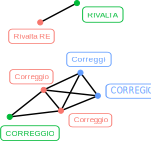
\includegraphics{ASSETS/composizione_dataset/reggio_series_graph_pmod.pdf}
        \caption*{Grafo dei \emph{match} di alcune serie di Reggio Emilia.}
      \end{figure}

    \end{column}
  \end{columns}
\end{frame}

\begin{frame}{\emph{Merging}: risultati}
  \begin{itemize}
    \item \(\approx 2500\) serie italiane di cui \(\approx 2350\) con almeno 5 anni di dati: \(\approx 3\) serie ogni \(\qty{100}{\kilo\meter^2}\);
    \item Disponibilità temporale sul trentennio significativamente superiore ai dataset sorgenti;
    \item Distribuzione geografica ben rappresentativa del territorio.
  \end{itemize}
  \begin{figure}
    \centering
    \small
    \begin{subfigure}[t]{0.45\textwidth}
      \small
      % Created by tikzDevice version 0.12.6 on 2025-04-07 02:23:31
% !TEX encoding = UTF-8 Unicode
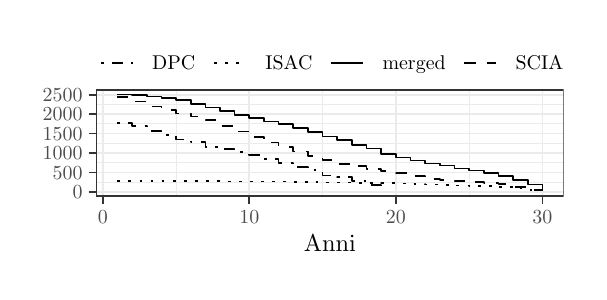
\begin{tikzpicture}[x=1pt,y=1pt]
\definecolor{fillColor}{RGB}{255,255,255}
\path[use as bounding box,fill=fillColor] (0,0) rectangle (199.17, 88.20);
\begin{scope}
\path[clip] (  0.00,  0.00) rectangle (199.17, 88.20);
\definecolor{drawColor}{RGB}{255,255,255}

\path[draw=drawColor,line width= 0.6pt,line join=round,line cap=round,fill=fillColor] (  0.00,  0.00) rectangle (199.17, 88.20);
\end{scope}
\begin{scope}
\path[clip] ( 24.75, 27.29) rectangle (193.67, 65.79);
\definecolor{fillColor}{RGB}{255,255,255}

\path[fill=fillColor] ( 24.75, 27.29) rectangle (193.67, 65.79);
\definecolor{drawColor}{gray}{0.92}

\path[draw=drawColor,line width= 0.3pt,line join=round] ( 24.75, 32.33) --
	(193.67, 32.33);

\path[draw=drawColor,line width= 0.3pt,line join=round] ( 24.75, 39.36) --
	(193.67, 39.36);

\path[draw=drawColor,line width= 0.3pt,line join=round] ( 24.75, 46.40) --
	(193.67, 46.40);

\path[draw=drawColor,line width= 0.3pt,line join=round] ( 24.75, 53.43) --
	(193.67, 53.43);

\path[draw=drawColor,line width= 0.3pt,line join=round] ( 24.75, 60.46) --
	(193.67, 60.46);

\path[draw=drawColor,line width= 0.3pt,line join=round] ( 53.61, 27.29) --
	( 53.61, 65.79);

\path[draw=drawColor,line width= 0.3pt,line join=round] (106.56, 27.29) --
	(106.56, 65.79);

\path[draw=drawColor,line width= 0.3pt,line join=round] (159.51, 27.29) --
	(159.51, 65.79);

\path[draw=drawColor,line width= 0.6pt,line join=round] ( 24.75, 28.81) --
	(193.67, 28.81);

\path[draw=drawColor,line width= 0.6pt,line join=round] ( 24.75, 35.85) --
	(193.67, 35.85);

\path[draw=drawColor,line width= 0.6pt,line join=round] ( 24.75, 42.88) --
	(193.67, 42.88);

\path[draw=drawColor,line width= 0.6pt,line join=round] ( 24.75, 49.91) --
	(193.67, 49.91);

\path[draw=drawColor,line width= 0.6pt,line join=round] ( 24.75, 56.95) --
	(193.67, 56.95);

\path[draw=drawColor,line width= 0.6pt,line join=round] ( 24.75, 63.98) --
	(193.67, 63.98);

\path[draw=drawColor,line width= 0.6pt,line join=round] ( 27.13, 27.29) --
	( 27.13, 65.79);

\path[draw=drawColor,line width= 0.6pt,line join=round] ( 80.09, 27.29) --
	( 80.09, 65.79);

\path[draw=drawColor,line width= 0.6pt,line join=round] (133.04, 27.29) --
	(133.04, 65.79);

\path[draw=drawColor,line width= 0.6pt,line join=round] (185.99, 27.29) --
	(185.99, 65.79);
\definecolor{drawColor}{RGB}{0,0,0}

\path[draw=drawColor,line width= 0.6pt,dash pattern=on 1pt off 3pt on 4pt off 3pt ,line join=round] ( 32.43, 53.80) --
	( 37.72, 53.80) --
	( 37.72, 52.61) --
	( 43.02, 52.61) --
	( 43.02, 50.93) --
	( 48.31, 50.93) --
	( 48.31, 49.34) --
	( 53.61, 49.34) --
	( 53.61, 47.73) --
	( 58.90, 47.73) --
	( 58.90, 46.83) --
	( 64.20, 46.83) --
	( 64.20, 45.06) --
	( 69.50, 45.06) --
	( 69.50, 44.46) --
	( 74.79, 44.46) --
	( 74.79, 43.19) --
	( 80.09, 43.19) --
	( 80.09, 42.15) --
	( 85.38, 42.15) --
	( 85.38, 40.83) --
	( 90.68, 40.83) --
	( 90.68, 39.35) --
	( 95.97, 39.35) --
	( 95.97, 37.77) --
	(101.27, 37.77) --
	(101.27, 36.69) --
	(106.56, 36.69) --
	(106.56, 34.83) --
	(111.86, 34.83) --
	(111.86, 34.22) --
	(117.15, 34.22) --
	(117.15, 32.77) --
	(122.45, 32.77) --
	(122.45, 31.37) --
	(127.74, 31.37) --
	(127.74, 29.53);

\path[draw=drawColor,line width= 0.6pt,dash pattern=on 1pt off 3pt ,line join=round] ( 32.43, 32.72) --
	( 37.72, 32.72) --
	( 37.72, 32.72) --
	( 43.02, 32.72) --
	( 43.02, 32.72) --
	( 48.31, 32.72) --
	( 48.31, 32.72) --
	( 53.61, 32.72) --
	( 53.61, 32.72) --
	( 58.90, 32.72) --
	( 58.90, 32.70) --
	( 64.20, 32.70) --
	( 64.20, 32.68) --
	( 69.50, 32.68) --
	( 69.50, 32.65) --
	( 74.79, 32.65) --
	( 74.79, 32.63) --
	( 80.09, 32.63) --
	( 80.09, 32.63) --
	( 85.38, 32.63) --
	( 85.38, 32.60) --
	( 90.68, 32.60) --
	( 90.68, 32.57) --
	( 95.97, 32.57) --
	( 95.97, 32.48) --
	(101.27, 32.48) --
	(101.27, 32.36) --
	(106.56, 32.36) --
	(106.56, 32.26) --
	(111.86, 32.26) --
	(111.86, 32.20) --
	(117.15, 32.20) --
	(117.15, 32.16) --
	(122.45, 32.16) --
	(122.45, 32.12) --
	(127.74, 32.12) --
	(127.74, 32.01) --
	(133.04, 32.01) --
	(133.04, 31.92) --
	(138.33, 31.92) --
	(138.33, 31.75) --
	(143.63, 31.75) --
	(143.63, 31.58) --
	(148.92, 31.58) --
	(148.92, 31.44) --
	(154.22, 31.44) --
	(154.22, 31.22) --
	(159.51, 31.22) --
	(159.51, 31.09) --
	(164.81, 31.09) --
	(164.81, 30.92) --
	(170.11, 30.92) --
	(170.11, 30.56) --
	(175.40, 30.56) --
	(175.40, 30.09) --
	(180.70, 30.09) --
	(180.70, 29.66) --
	(185.99, 29.66) --
	(185.99, 29.04);

\path[draw=drawColor,line width= 0.6pt,line join=round] ( 32.43, 64.04) --
	( 37.72, 64.04) --
	( 37.72, 63.94) --
	( 43.02, 63.94) --
	( 43.02, 63.39) --
	( 48.31, 63.39) --
	( 48.31, 62.74) --
	( 53.61, 62.74) --
	( 53.61, 62.01) --
	( 58.90, 62.01) --
	( 58.90, 60.72) --
	( 64.20, 60.72) --
	( 64.20, 59.34) --
	( 69.50, 59.34) --
	( 69.50, 58.04) --
	( 74.79, 58.04) --
	( 74.79, 56.64) --
	( 80.09, 56.64) --
	( 80.09, 55.48) --
	( 85.38, 55.48) --
	( 85.38, 54.29) --
	( 90.68, 54.29) --
	( 90.68, 53.29) --
	( 95.97, 53.29) --
	( 95.97, 51.95) --
	(101.27, 51.95) --
	(101.27, 50.46) --
	(106.56, 50.46) --
	(106.56, 48.90) --
	(111.86, 48.90) --
	(111.86, 47.54) --
	(117.15, 47.54) --
	(117.15, 45.85) --
	(122.45, 45.85) --
	(122.45, 44.50) --
	(127.74, 44.50) --
	(127.74, 42.65) --
	(133.04, 42.65) --
	(133.04, 41.26) --
	(138.33, 41.26) --
	(138.33, 40.24) --
	(143.63, 40.24) --
	(143.63, 39.11) --
	(148.92, 39.11) --
	(148.92, 38.35) --
	(154.22, 38.35) --
	(154.22, 37.28) --
	(159.51, 37.28) --
	(159.51, 36.59) --
	(164.81, 36.59) --
	(164.81, 35.62) --
	(170.11, 35.62) --
	(170.11, 34.57) --
	(175.40, 34.57) --
	(175.40, 33.24) --
	(180.70, 33.24) --
	(180.70, 31.50) --
	(185.99, 31.50) --
	(185.99, 29.63);

\path[draw=drawColor,line width= 0.6pt,dash pattern=on 4pt off 4pt ,line join=round] ( 32.43, 63.12) --
	( 37.72, 63.12) --
	( 37.72, 61.49) --
	( 43.02, 61.49) --
	( 43.02, 59.76) --
	( 48.31, 59.76) --
	( 48.31, 58.47) --
	( 53.61, 58.47) --
	( 53.61, 57.24) --
	( 58.90, 57.24) --
	( 58.90, 56.16) --
	( 64.20, 56.16) --
	( 64.20, 54.88) --
	( 69.50, 54.88) --
	( 69.50, 52.74) --
	( 74.79, 52.74) --
	( 74.79, 50.64) --
	( 80.09, 50.64) --
	( 80.09, 48.60) --
	( 85.38, 48.60) --
	( 85.38, 46.68) --
	( 90.68, 46.68) --
	( 90.68, 45.17) --
	( 95.97, 45.17) --
	( 95.97, 43.44) --
	(101.27, 43.44) --
	(101.27, 41.91) --
	(106.56, 41.91) --
	(106.56, 40.50) --
	(111.86, 40.50) --
	(111.86, 39.04) --
	(117.15, 39.04) --
	(117.15, 38.11) --
	(122.45, 38.11) --
	(122.45, 37.21) --
	(127.74, 37.21) --
	(127.74, 36.31) --
	(133.04, 36.31) --
	(133.04, 35.62) --
	(138.33, 35.62) --
	(138.33, 34.65) --
	(143.63, 34.65) --
	(143.63, 33.50) --
	(148.92, 33.50) --
	(148.92, 33.16) --
	(154.22, 33.16) --
	(154.22, 32.70) --
	(159.51, 32.70) --
	(159.51, 32.34) --
	(164.81, 32.34) --
	(164.81, 32.05) --
	(170.11, 32.05) --
	(170.11, 31.63) --
	(175.40, 31.63) --
	(175.40, 30.61) --
	(180.70, 30.61) --
	(180.70, 29.47) --
	(185.99, 29.47) --
	(185.99, 29.07);
\definecolor{drawColor}{gray}{0.20}

\path[draw=drawColor,line width= 0.6pt,line join=round,line cap=round] ( 24.75, 27.29) rectangle (193.67, 65.79);
\end{scope}
\begin{scope}
\path[clip] (  0.00,  0.00) rectangle (199.17, 88.20);
\definecolor{drawColor}{gray}{0.30}

\node[text=drawColor,anchor=base east,inner sep=0pt, outer sep=0pt, scale=  0.72] at ( 19.80, 26.35) {0};

\node[text=drawColor,anchor=base east,inner sep=0pt, outer sep=0pt, scale=  0.72] at ( 19.80, 33.38) {500};

\node[text=drawColor,anchor=base east,inner sep=0pt, outer sep=0pt, scale=  0.72] at ( 19.80, 40.42) {1000};

\node[text=drawColor,anchor=base east,inner sep=0pt, outer sep=0pt, scale=  0.72] at ( 19.80, 47.45) {1500};

\node[text=drawColor,anchor=base east,inner sep=0pt, outer sep=0pt, scale=  0.72] at ( 19.80, 54.48) {2000};

\node[text=drawColor,anchor=base east,inner sep=0pt, outer sep=0pt, scale=  0.72] at ( 19.80, 61.52) {2500};
\end{scope}
\begin{scope}
\path[clip] (  0.00,  0.00) rectangle (199.17, 88.20);
\definecolor{drawColor}{gray}{0.20}

\path[draw=drawColor,line width= 0.6pt,line join=round] ( 22.00, 28.81) --
	( 24.75, 28.81);

\path[draw=drawColor,line width= 0.6pt,line join=round] ( 22.00, 35.85) --
	( 24.75, 35.85);

\path[draw=drawColor,line width= 0.6pt,line join=round] ( 22.00, 42.88) --
	( 24.75, 42.88);

\path[draw=drawColor,line width= 0.6pt,line join=round] ( 22.00, 49.91) --
	( 24.75, 49.91);

\path[draw=drawColor,line width= 0.6pt,line join=round] ( 22.00, 56.95) --
	( 24.75, 56.95);

\path[draw=drawColor,line width= 0.6pt,line join=round] ( 22.00, 63.98) --
	( 24.75, 63.98);
\end{scope}
\begin{scope}
\path[clip] (  0.00,  0.00) rectangle (199.17, 88.20);
\definecolor{drawColor}{gray}{0.20}

\path[draw=drawColor,line width= 0.6pt,line join=round] ( 27.13, 24.54) --
	( 27.13, 27.29);

\path[draw=drawColor,line width= 0.6pt,line join=round] ( 80.09, 24.54) --
	( 80.09, 27.29);

\path[draw=drawColor,line width= 0.6pt,line join=round] (133.04, 24.54) --
	(133.04, 27.29);

\path[draw=drawColor,line width= 0.6pt,line join=round] (185.99, 24.54) --
	(185.99, 27.29);
\end{scope}
\begin{scope}
\path[clip] (  0.00,  0.00) rectangle (199.17, 88.20);
\definecolor{drawColor}{gray}{0.30}

\node[text=drawColor,anchor=base,inner sep=0pt, outer sep=0pt, scale=  0.72] at ( 27.13, 17.41) {0};

\node[text=drawColor,anchor=base,inner sep=0pt, outer sep=0pt, scale=  0.72] at ( 80.09, 17.41) {10};

\node[text=drawColor,anchor=base,inner sep=0pt, outer sep=0pt, scale=  0.72] at (133.04, 17.41) {20};

\node[text=drawColor,anchor=base,inner sep=0pt, outer sep=0pt, scale=  0.72] at (185.99, 17.41) {30};
\end{scope}
\begin{scope}
\path[clip] (  0.00,  0.00) rectangle (199.17, 88.20);
\definecolor{drawColor}{RGB}{0,0,0}

\node[text=drawColor,anchor=base,inner sep=0pt, outer sep=0pt, scale=  0.88] at (109.21,  7.21) {Anni};
\end{scope}
\begin{scope}
\path[clip] (  0.00,  0.00) rectangle (199.17, 88.20);
\definecolor{fillColor}{RGB}{255,255,255}

\path[fill=fillColor] ( 24.99, 76.79) rectangle (193.42, 82.70);
\end{scope}
\begin{scope}
\path[clip] (  0.00,  0.00) rectangle (199.17, 88.20);
\definecolor{fillColor}{RGB}{255,255,255}

\path[fill=fillColor] ( 24.99, 68.25) rectangle ( 39.45, 82.70);
\end{scope}
\begin{scope}
\path[clip] (  0.00,  0.00) rectangle (199.17, 88.20);
\definecolor{drawColor}{RGB}{0,0,0}

\path[draw=drawColor,line width= 0.6pt,dash pattern=on 1pt off 3pt on 4pt off 3pt ,line join=round] ( 26.44, 75.48) -- ( 38.00, 75.48);
\end{scope}
\begin{scope}
\path[clip] (  0.00,  0.00) rectangle (199.17, 88.20);
\definecolor{fillColor}{RGB}{255,255,255}

\path[fill=fillColor] ( 65.94, 68.25) rectangle ( 80.39, 82.70);
\end{scope}
\begin{scope}
\path[clip] (  0.00,  0.00) rectangle (199.17, 88.20);
\definecolor{drawColor}{RGB}{0,0,0}

\path[draw=drawColor,line width= 0.6pt,dash pattern=on 1pt off 3pt ,line join=round] ( 67.39, 75.48) -- ( 78.95, 75.48);
\end{scope}
\begin{scope}
\path[clip] (  0.00,  0.00) rectangle (199.17, 88.20);
\definecolor{fillColor}{RGB}{255,255,255}

\path[fill=fillColor] (108.28, 68.25) rectangle (122.73, 82.70);
\end{scope}
\begin{scope}
\path[clip] (  0.00,  0.00) rectangle (199.17, 88.20);
\definecolor{drawColor}{RGB}{0,0,0}

\path[draw=drawColor,line width= 0.6pt,line join=round] (109.72, 75.48) -- (121.28, 75.48);
\end{scope}
\begin{scope}
\path[clip] (  0.00,  0.00) rectangle (199.17, 88.20);
\definecolor{fillColor}{RGB}{255,255,255}

\path[fill=fillColor] (156.39, 68.25) rectangle (170.84, 82.70);
\end{scope}
\begin{scope}
\path[clip] (  0.00,  0.00) rectangle (199.17, 88.20);
\definecolor{drawColor}{RGB}{0,0,0}

\path[draw=drawColor,line width= 0.6pt,dash pattern=on 4pt off 4pt ,line join=round] (157.84, 75.48) -- (169.40, 75.48);
\end{scope}
\begin{scope}
\path[clip] (  0.00,  0.00) rectangle (199.17, 88.20);
\definecolor{drawColor}{RGB}{0,0,0}

\node[text=drawColor,anchor=base west,inner sep=0pt, outer sep=0pt, scale=  0.72] at ( 44.95, 73.01) {DPC};
\end{scope}
\begin{scope}
\path[clip] (  0.00,  0.00) rectangle (199.17, 88.20);
\definecolor{drawColor}{RGB}{0,0,0}

\node[text=drawColor,anchor=base west,inner sep=0pt, outer sep=0pt, scale=  0.72] at ( 85.89, 73.01) {ISAC};
\end{scope}
\begin{scope}
\path[clip] (  0.00,  0.00) rectangle (199.17, 88.20);
\definecolor{drawColor}{RGB}{0,0,0}

\node[text=drawColor,anchor=base west,inner sep=0pt, outer sep=0pt, scale=  0.72] at (128.23, 73.01) {merged};
\end{scope}
\begin{scope}
\path[clip] (  0.00,  0.00) rectangle (199.17, 88.20);
\definecolor{drawColor}{RGB}{0,0,0}

\node[text=drawColor,anchor=base west,inner sep=0pt, outer sep=0pt, scale=  0.72] at (176.34, 73.01) {SCIA};
\end{scope}
\end{tikzpicture}

      \caption*{Numero di serie disponibili con almeno n anni.}
    \end{subfigure}
    \hfill
    \begin{subfigure}[t]{0.45\textwidth}
      \small
      % Created by tikzDevice version 0.12.6 on 2025-04-07 21:10:49
% !TEX encoding = UTF-8 Unicode
\begin{tikzpicture}[x=1pt,y=1pt]
  \definecolor{fillColor}{RGB}{255,255,255}
  \path[use as bounding box,fill=fillColor] (0,0) rectangle (170.72, 88.20);
  \begin{scope}
    \path[clip] (  0.00,  0.00) rectangle (170.72, 88.20);
    \definecolor{drawColor}{RGB}{255,255,255}

    \path[draw=drawColor,line width= 0.6pt,line join=round,line cap=round,fill=fillColor] (  0.00,  0.00) rectangle (170.72, 88.20);
  \end{scope}
  \begin{scope}
    \path[clip] ( 44.69, 27.29) rectangle (165.22, 65.79);
    \definecolor{fillColor}{RGB}{255,255,255}

    \path[fill=fillColor] ( 44.69, 27.29) rectangle (165.22, 65.79);
    \definecolor{drawColor}{gray}{0.92}

    \path[draw=drawColor,line width= 0.3pt,line join=round] ( 44.69, 33.71) --
    (165.22, 33.71);

    \path[draw=drawColor,line width= 0.3pt,line join=round] ( 44.69, 43.07) --
    (165.22, 43.07);

    \path[draw=drawColor,line width= 0.3pt,line join=round] ( 44.69, 52.42) --
    (165.22, 52.42);

    \path[draw=drawColor,line width= 0.3pt,line join=round] ( 44.69, 61.77) --
    (165.22, 61.77);

    \path[draw=drawColor,line width= 0.3pt,line join=round] ( 64.58, 27.29) --
    ( 64.58, 65.79);

    \path[draw=drawColor,line width= 0.3pt,line join=round] ( 87.65, 27.29) --
    ( 87.65, 65.79);

    \path[draw=drawColor,line width= 0.3pt,line join=round] (110.72, 27.29) --
    (110.72, 65.79);

    \path[draw=drawColor,line width= 0.3pt,line join=round] (133.79, 27.29) --
    (133.79, 65.79);

    \path[draw=drawColor,line width= 0.3pt,line join=round] (156.85, 27.29) --
    (156.85, 65.79);

    \path[draw=drawColor,line width= 0.6pt,line join=round] ( 44.69, 29.04) --
    (165.22, 29.04);

    \path[draw=drawColor,line width= 0.6pt,line join=round] ( 44.69, 38.39) --
    (165.22, 38.39);

    \path[draw=drawColor,line width= 0.6pt,line join=round] ( 44.69, 47.74) --
    (165.22, 47.74);

    \path[draw=drawColor,line width= 0.6pt,line join=round] ( 44.69, 57.09) --
    (165.22, 57.09);

    \path[draw=drawColor,line width= 0.6pt,line join=round] ( 53.05, 27.29) --
    ( 53.05, 65.79);

    \path[draw=drawColor,line width= 0.6pt,line join=round] ( 76.12, 27.29) --
    ( 76.12, 65.79);

    \path[draw=drawColor,line width= 0.6pt,line join=round] ( 99.18, 27.29) --
    ( 99.18, 65.79);

    \path[draw=drawColor,line width= 0.6pt,line join=round] (122.25, 27.29) --
    (122.25, 65.79);

    \path[draw=drawColor,line width= 0.6pt,line join=round] (145.32, 27.29) --
    (145.32, 65.79);
    \definecolor{fillColor}{RGB}{248,118,109}

    \path[fill=fillColor] ( 50.17, 29.04) rectangle ( 53.05, 64.04);

    \path[fill=fillColor] ( 55.93, 29.04) rectangle ( 58.82, 59.51);

    \path[fill=fillColor] ( 61.70, 29.04) rectangle ( 64.58, 45.50);

    \path[fill=fillColor] ( 67.47, 29.04) rectangle ( 70.35, 39.27);

    \path[fill=fillColor] ( 73.23, 29.04) rectangle ( 76.12, 36.38);

    \path[fill=fillColor] ( 79.00, 29.04) rectangle ( 81.88, 34.63);

    \path[fill=fillColor] ( 84.77, 29.04) rectangle ( 87.65, 33.73);

    \path[fill=fillColor] ( 90.53, 29.04) rectangle ( 93.42, 33.08);

    \path[fill=fillColor] ( 96.30, 29.04) rectangle ( 99.18, 32.63);

    \path[fill=fillColor] (102.07, 29.04) rectangle (104.95, 31.97);

    \path[fill=fillColor] (107.84, 29.04) rectangle (110.72, 31.20);

    \path[fill=fillColor] (113.60, 29.04) rectangle (116.49, 30.35);

    \path[fill=fillColor] (119.37, 29.04) rectangle (122.25, 29.61);

    \path[fill=fillColor] (125.14, 29.04) rectangle (128.02, 29.24);

    \path[fill=fillColor] (130.90, 29.04) rectangle (133.79, 29.09);

    \path[fill=fillColor] (136.67, 29.04) rectangle (139.55, 29.06);

    \path[fill=fillColor] (142.44, 29.04) rectangle (145.32, 29.04);

    \path[fill=fillColor] (148.20, 29.04) rectangle (151.09, 29.04);

    \path[fill=fillColor] (153.97, 29.04) rectangle (156.85, 29.04);
    \definecolor{fillColor}{RGB}{0,191,196}

    \path[fill=fillColor] ( 53.05, 29.04) rectangle ( 55.93, 58.35);

    \path[fill=fillColor] ( 58.82, 29.04) rectangle ( 61.70, 56.76);

    \path[fill=fillColor] ( 64.58, 29.04) rectangle ( 67.47, 46.55);

    \path[fill=fillColor] ( 70.35, 29.04) rectangle ( 73.23, 41.73);

    \path[fill=fillColor] ( 76.12, 29.04) rectangle ( 79.00, 38.08);

    \path[fill=fillColor] ( 81.88, 29.04) rectangle ( 84.77, 37.29);

    \path[fill=fillColor] ( 87.65, 29.04) rectangle ( 90.53, 34.49);

    \path[fill=fillColor] ( 93.42, 29.04) rectangle ( 96.30, 34.22);

    \path[fill=fillColor] ( 99.18, 29.04) rectangle (102.07, 33.06);

    \path[fill=fillColor] (104.95, 29.04) rectangle (107.84, 31.68);

    \path[fill=fillColor] (110.72, 29.04) rectangle (113.60, 30.10);

    \path[fill=fillColor] (116.49, 29.04) rectangle (119.37, 29.78);

    \path[fill=fillColor] (122.25, 29.04) rectangle (125.14, 29.67);

    \path[fill=fillColor] (128.02, 29.04) rectangle (130.90, 29.30);

    \path[fill=fillColor] (133.79, 29.04) rectangle (136.67, 29.14);

    \path[fill=fillColor] (139.55, 29.04) rectangle (142.44, 29.04);

    \path[fill=fillColor] (145.32, 29.04) rectangle (148.20, 29.04);

    \path[fill=fillColor] (151.09, 29.04) rectangle (153.97, 29.04);

    \path[fill=fillColor] (156.85, 29.04) rectangle (159.74, 29.09);
    \definecolor{drawColor}{gray}{0.20}

    \path[draw=drawColor,line width= 0.6pt,line join=round,line cap=round] ( 44.69, 27.29) rectangle (165.22, 65.79);
  \end{scope}
  \begin{scope}
    \path[clip] (  0.00,  0.00) rectangle (170.72, 88.20);
    \definecolor{drawColor}{gray}{0.30}

    \node[text=drawColor,anchor=base east,inner sep=0pt, outer sep=0pt, scale=  0.72] at ( 39.74, 26.58) {0e+00};

    \node[text=drawColor,anchor=base east,inner sep=0pt, outer sep=0pt, scale=  0.72] at ( 39.74, 35.93) {3e-04};

    \node[text=drawColor,anchor=base east,inner sep=0pt, outer sep=0pt, scale=  0.72] at ( 39.74, 45.28) {6e-04};

    \node[text=drawColor,anchor=base east,inner sep=0pt, outer sep=0pt, scale=  0.72] at ( 39.74, 54.63) {9e-04};
  \end{scope}
  \begin{scope}
    \path[clip] (  0.00,  0.00) rectangle (170.72, 88.20);
    \definecolor{drawColor}{gray}{0.20}

    \path[draw=drawColor,line width= 0.6pt,line join=round] ( 41.94, 29.04) --
    ( 44.69, 29.04);

    \path[draw=drawColor,line width= 0.6pt,line join=round] ( 41.94, 38.39) --
    ( 44.69, 38.39);

    \path[draw=drawColor,line width= 0.6pt,line join=round] ( 41.94, 47.74) --
    ( 44.69, 47.74);

    \path[draw=drawColor,line width= 0.6pt,line join=round] ( 41.94, 57.09) --
    ( 44.69, 57.09);
  \end{scope}
  \begin{scope}
    \path[clip] (  0.00,  0.00) rectangle (170.72, 88.20);
    \definecolor{drawColor}{gray}{0.20}

    \path[draw=drawColor,line width= 0.6pt,line join=round] ( 53.05, 24.54) --
    ( 53.05, 27.29);

    \path[draw=drawColor,line width= 0.6pt,line join=round] ( 76.12, 24.54) --
    ( 76.12, 27.29);

    \path[draw=drawColor,line width= 0.6pt,line join=round] ( 99.18, 24.54) --
    ( 99.18, 27.29);

    \path[draw=drawColor,line width= 0.6pt,line join=round] (122.25, 24.54) --
    (122.25, 27.29);

    \path[draw=drawColor,line width= 0.6pt,line join=round] (145.32, 24.54) --
    (145.32, 27.29);
  \end{scope}
  \begin{scope}
    \path[clip] (  0.00,  0.00) rectangle (170.72, 88.20);
    \definecolor{drawColor}{gray}{0.30}

    \node[text=drawColor,anchor=base,inner sep=0pt, outer sep=0pt, scale=  0.72] at ( 53.05, 17.41) {0};

    \node[text=drawColor,anchor=base,inner sep=0pt, outer sep=0pt, scale=  0.72] at ( 76.12, 17.41) {1000};

    \node[text=drawColor,anchor=base,inner sep=0pt, outer sep=0pt, scale=  0.72] at ( 99.18, 17.41) {2000};

    \node[text=drawColor,anchor=base,inner sep=0pt, outer sep=0pt, scale=  0.72] at (122.25, 17.41) {3000};

    \node[text=drawColor,anchor=base,inner sep=0pt, outer sep=0pt, scale=  0.72] at (145.32, 17.41) {4000};
  \end{scope}
  \begin{scope}
    \path[clip] (  0.00,  0.00) rectangle (170.72, 88.20);
    \definecolor{drawColor}{RGB}{0,0,0}

    \node[text=drawColor,anchor=base,inner sep=0pt, outer sep=0pt, scale=  0.88] at (104.95,  7.21) {Elevazione [m]};
  \end{scope}
  \begin{scope}
    \path[clip] (  0.00,  0.00) rectangle (170.72, 88.20);
    \definecolor{drawColor}{RGB}{0,0,0}

    \node[text=drawColor,rotate= 90.00,anchor=base,inner sep=0pt, outer sep=0pt, scale=  0.88] at ( 11.56, 46.54) {Densità [\unit{\metre^{-1}}]};
  \end{scope}
  \begin{scope}
    \path[clip] (  0.00,  0.00) rectangle (170.72, 88.20);
    \definecolor{fillColor}{RGB}{255,255,255}

    \path[fill=fillColor] ( 64.35, 76.79) rectangle (145.55, 82.70);
  \end{scope}
  \begin{scope}
    \path[clip] (  0.00,  0.00) rectangle (170.72, 88.20);
    \definecolor{fillColor}{RGB}{255,255,255}

    \path[fill=fillColor] ( 64.35, 68.25) rectangle ( 78.81, 82.70);
  \end{scope}
  \begin{scope}
    \path[clip] (  0.00,  0.00) rectangle (170.72, 88.20);
    \definecolor{fillColor}{RGB}{248,118,109}

    \path[fill=fillColor] ( 65.06, 68.96) rectangle ( 78.10, 81.99);
  \end{scope}
  \begin{scope}
    \path[clip] (  0.00,  0.00) rectangle (170.72, 88.20);
    \definecolor{fillColor}{RGB}{255,255,255}

    \path[fill=fillColor] (102.92, 68.25) rectangle (117.37, 82.70);
  \end{scope}
  \begin{scope}
    \path[clip] (  0.00,  0.00) rectangle (170.72, 88.20);
    \definecolor{fillColor}{RGB}{0,191,196}

    \path[fill=fillColor] (103.63, 68.96) rectangle (116.66, 81.99);
  \end{scope}
  \begin{scope}
    \path[clip] (  0.00,  0.00) rectangle (170.72, 88.20);
    \definecolor{drawColor}{RGB}{0,0,0}

    \node[text=drawColor,anchor=base west,inner sep=0pt, outer sep=0pt, scale=  0.72] at ( 84.31, 73.01) {dem};
  \end{scope}
  \begin{scope}
    \path[clip] (  0.00,  0.00) rectangle (170.72, 88.20);
    \definecolor{drawColor}{RGB}{0,0,0}

    \node[text=drawColor,anchor=base west,inner sep=0pt, outer sep=0pt, scale=  0.72] at (122.87, 73.01) {dataset};
  \end{scope}
\end{tikzpicture}

      \caption*{Distribuzione in quota delle serie ottenute.}
    \end{subfigure}
  \end{figure}
\end{frame}

\begin{frame}{Controllo qualità ed omogeneizzazione}
  \begin{enumerate}
    \item Controllo degli errori palesi: \(\lvert \mathrm{T} \rvert > \qty{50}{\degreeCelsius}\) e dati ripetuti;
    \item Confronto con serie sintetiche ERA5;
    \item Confronto con serie limitrofe;
    \item \emph{Gap filling} dei dati mancanti.
  \end{enumerate}
\end{frame}